
\chapter{Partial Derivatives}

\section*{Introduction}

In our journey through calculus, we now extend our exploration to functions of several variables, building upon the foundations of single-variable calculus and vector-valued functions. Previously, we focused on how quantities change along curves, analyzing motion within a one-dimensional framework. However, many real-world phenomena depend on multiple variables simultaneously—such as temperature variations across a surface or pressure changes within a fluid. \\ \\ This chapter delves into multivariable functions, where inputs and outputs exist in higher-dimensional spaces. We begin by examining how to visualize these functions using level curves and surfaces, setting the stage for understanding limits and continuity in higher dimensions. Central to our study are partial derivatives, which measure how a function changes with respect to one variable while keeping others constant. This generalizes the concept of derivatives from single-variable calculus and provides insights into the behavior of multivariable functions. We will learn to compute partial derivatives and explore higher-order derivatives, including Clairaut's Theorem on mixed partial derivatives. \\ \\ Building on these concepts, we introduce directional derivatives and gradient vectors, which reveal how functions change in any specified direction. The gradient vector, in particular, points in the direction of the greatest rate of increase of the function and is fundamental in solving optimization problems. By integrating (pun intended) these new ideas with earlier concepts, we enhance our mathematical toolkit, enabling us to tackle complex problems involving multiple variables. The study of partial derivatives not only deepens our understanding of calculus but also prepares us for advanced topics in applied mathematics and real-world applications.



\newpage 


\lecture{Functions of Several Variables}

\noindent In previous chapters, we have explored functions of a single variable and vector-valued functions, which map a single parameter to a vector in space. Now, we extend our study to \textit{functions of several variables}, a fundamental concept in multivariable calculus that allows us to model and analyze phenomena where the output depends on multiple inputs. This lecture introduces the concept of functions of several variables, examines their domains and ranges, and explores techniques for visualizing them through graphs and level curves.

\subsection*{Functions of Two Variables} \index{Functions of Two Variables}

\noindent A function of two variables is a rule that assigns to each ordered pair \( (x, y) \) in a subset of \( \mathbb{R}^2 \) a unique real number \( z = f(x, y) \). This can be thought of as a surface in three-dimensional space, where the height \( z \) above each point \( (x, y) \) represents the value of the function at that point. In mathematical terms, such a function can be expressed as \( f: \mathbb{R} \times \mathbb{R} \to \mathbb{R} \), where \( \mathbb{R} \times \mathbb{R} \) represents all possible ordered pairs \( (x, y) \) in two-dimensional space, and the output is a real number. To understand functions of two variables, recall our knowledge of single-variable functions \( y = f(x) \):
\begin{itemize}
    \item The graph of \( f(x) \) is a curve in two dimensions, where \( y \) represents the output for a given input \( x \).
    \item The domain is the set of all allowable \( x \)-values, and the range is the set of resulting \( y \)-values.
\end{itemize}
For functions of two variables, the domain is a subset of \( \mathbb{R}^2 \), typically a region in the \( xy \)-plane, and the range is a set of real numbers \( z \). Graphically, the function \( z = f(x, y) \) is represented as a surface in three-dimensional space. Functions of two variables appear naturally in many contexts that you may already be familiar with but haven't seen defined in the context of multivariate mathematics. For instance, here are some that you are certainly familiar with represented explicitly as multivariate functions.

\begin{itemize}
    \item \textbf{Density:} Density is defined as mass divided by volume, so density is a function of mass and volume:
    \[
    \rho = f(m, v) = \frac{m}{v}.
    \]
    \item \textbf{Einstein's Energy Equation:} Einstein's famous equation for relativistic energy depends on mass and velocity:
    \[
    E = f(m, v) = \frac{mc^2}{\sqrt{1 - \frac{v^2}{c^2}}},
    \]
    where \( c \) is the speed of light. Since \( c \) is constant, we typically consider energy as a function of the two variables \( m \) (mass) and \( v \) (velocity).
\item \textbf{Taco Bell}: \index{Taco-Related Examples} Suppose if I order some tacos for my family, we could represent this as such:
\[
\text{Cost} = f(J, E, A) = \left[J \cdot \frac{\$ d_1}{\text{\# Gorditas}} + E \cdot \frac{\$ d_2}{\text{\# Crunchwraps}} + A \cdot \frac{\$ d_3}{\text{\# Tacos}}\right] \cdot 1.08,
\]
where \( d_1, d_2, \) and \( d_3 \) represent the prices per Gordita Crunch, Crunchwrap Supreme, and Soft Taco, respectively, and the \( 1.08 \) accounts for an 8\% sales tax (I know, I know, I cheated and put a function of three variables for this one but the idea is the same). If I order 2 Gordita Crunches at \$4 each, my wife orders 1 Crunchwrap Supreme at \$5, and my son orders 3 Soft Tacos at \$2 each, the cost before tax is:
\[
\text{Pre-tax Cost} = f(2, 1, 3) = 2 \cdot 4 + 1 \cdot 5 + 3 \cdot 2 = 8 + 5 + 6 = 19.
\]
Including the 8\% sales tax, the total cost becomes:
\[
\text{Cost} = 19 \cdot 1.08 = 20.52.
\]

This is an example where the domain of the function \( f \) is restricted to natural numbers or zero denoted as $\mathbb{N}_0$, as we can only order whole numbers (or zero) of each item (e.g., 2 Gorditas, not 2.5). Thus, the function maps from $\mathbb{N}_0 \times \mathbb{N}_0 \times \mathbb{N}_0$ (the number of Gorditas, Crunchwraps, and Tacos) to $\mathbb{Q}$, the set of rational numbers representing the total cost:
\[
f: \mathbb{N}_0 \times \mathbb{N}_0 \times \mathbb{N}_0 \to \mathbb{Q}.
\]
\end{itemize}

\noindent These examples illustrate how functions of several variables naturally arise in physical, scientific, and taco-related incidences, enabling us to describe and analyze relationships involving multiple (and potentially delicious) inputs.

\exampleline
\begin{example}
Consider functions that describe relationships between physical quantities. Write three examples of famous equations where one quantity is expressed as a function of exactly two other variables. Clearly identify the function and its meaning.


\begin{solution}
Here are three examples:

\begin{enumerate}
    \item \textbf{Ohm's Law:} Voltage is a function of current and resistance:
    \[
    V = f(I, R) = I \cdot R,
    \]
    where \( V \) is the voltage, \( I \) is the current, and \( R \) is the resistance.

    \item \textbf{Power:} Power is a function of voltage and resistance:
    \[
    P = f(V, R) = \frac{V^2}{R},
    \]
    where \( P \) is the power dissipated, \( V \) is the voltage, and \( R \) is the resistance.

    \item \textbf{Kinetic Energy:} Kinetic energy is a function of mass and velocity:
    \[
    KE = f(m, v) = \frac{1}{2} m v^2,
    \]
    where \( KE \) is the kinetic energy, \( m \) is the mass, and \( v \) is the velocity.
\end{enumerate}
\end{solution}
\end{example}
\exampleline

\subsubsection*{Domain and Range}

\noindent The \textbf{domain} of a function \( f(x, y) \) consists of all ordered pairs \( (x, y) \) for which \( f(x, y) \) is defined. The \textbf{range} is the set of all real numbers \( z \) that \( f(x, y) \) takes on as \( (x, y) \) varies over the domain. In single-variable calculus, determining the domain and range of a function involves identifying the set of input values \( x \) for which the function is defined and the corresponding set of output values \( y = f(x) \). This extends naturally to functions of several variables. \\ \\ For functions of two variables, the domain is often described as a subset of \( \mathbb{R}^2 \), or more generally \( S \times S \), where \( S \) is a set of values satisfying specific restrictions. For instance, if \( f(x, y) = \frac{1}{x^2 + y^2} \), the domain excludes the origin, and we can write:
\[
\dom f = \{(x, y) \in \mathbb{R}^2 \mid x^2 + y^2 \neq 0\}.
\]
More generally, for a function \( g(x, y) \), the domain can be expressed as:
\[
\dom g = \{(x, y) \in S \times S \mid \text{restrictions on } x \text{ and } y\}.
\]

\noindent To describe the range, there is less standardized notation, but for this text, we will use:
\[
\range f = \{z \in C \mid z = f(x, y) \text{ for some } (x, y) \in \dom f \}.
\]
Here, \( C \) represents the codomain of \( f \), which is often \( \mathbb{R} \) for real-valued functions. While this notation is not universally standard, it provides a concise way to describe the range, and we will adopt it for clarity in this context. For example, if \( f(x, y) = x^2 + y^2 \), we can write:
\[
\range f = \{z \in \mathbb{R}_{\geq 0} \mid z = x^2 + y^2 \text{ for some } (x, y) \in \mathbb{R}^2 \}.
\]
\noindent or just simply
\[
\range f = [0, \infty).
\]

\paragraph{Techniques for Determining the Domain}

Here are some general steps and considerations for finding the domain of \( f(x, y) \):

\begin{enumerate}
    \item \textbf{Identify Undefined Expressions:} Just like in single-variable functions, we need to find values of \( (x, y) \) that make the function undefined.
        \begin{itemize}
            \item \textit{Denominators:} Ensure that any denominators are not equal to zero. For example, \( f(x, y) = \frac{1}{x - y} \) is undefined at \( x = y \).
            \item \textit{Square Roots and Even Roots:} The radicand (expression under the root) must be non-negative. For example, \( g(x, y) = \sqrt{1 - x^2 - y^2} \) is defined where \( x^2 + y^2 \leq 1 \).
            \item \textit{Logarithms:} The argument of a logarithmic function must be positive. For instance, \( h(x, y) = \ln(x + y) \) requires \( x + y > 0 \).
            \item \textit{Trigonometric Functions:} For inverse trigonometric functions, consider their specific restrictions. For instance, \( \arcsin(x + y) \) is defined when \( -1 \leq x + y \leq 1 \).
        \end{itemize}
    \item \textbf{Set Notation:} Use inequalities or equations to describe the domain. For example, the domain of \( k(x, y) = \sqrt{1 - x^2 - y^2} \) can be written as:
    \[
    \dom k = \{(x, y) \in \mathbb{R}^2 \mid x^2 + y^2 \leq 1\}.
    \]
    \item \textbf{Graphical Representation:} Visualize the domain in the \( xy \)-plane to better understand the set of allowed inputs. For example, the domain of \( k(x, y) \) corresponds to the unit disk.
\end{enumerate}

\exampleline
\begin{example}
Determine the domain and range of the following functions using proper notation:
\begin{enumerate}
    \item \( f(x, y) = \frac{1}{x + y} \)
    \item \( g(x, y) = \frac{\ln(x - y)}{\sqrt{x^2 + y^2 - 4}} \)
\end{enumerate}


\begin{solution}
\begin{enumerate}
    \item For \( f(x, y) = \frac{1}{x + y} \):
    \begin{enumerate}
        \item \textbf{Domain:} The function is undefined when the denominator is zero:
        \[
        x + y \neq 0.
        \]
        Thus, the domain is:
        \[
        \dom f = \{(x, y) \in \mathbb{R}^2 \mid x + y \neq 0\}.
        \]
        \item \textbf{Range:} The function \( f(x, y) \) can take any nonzero real value because the reciprocal of \( x + y \) is well-defined for all nonzero values of \( x + y \). Since \( f(x, y) = \frac{1}{x + y} \), the output cannot be zero because there is no \( x + y \) for which \( \frac{1}{x + y} = 0 \). The range is:
        \[
        \range f = \mathbb{R} \setminus \{0\}.
        \]
    \end{enumerate}

    \item For \( g(x, y) = \frac{\ln(x - y)}{\sqrt{x^2 + y^2 - 4}} \):
    \begin{enumerate}
        \item \textbf{Domain:} The function is defined when both the logarithmic and square root expressions are valid:
        \begin{itemize}
            \item The logarithmic term \( \ln(x - y) \) requires:
            \[
            x - y > 0.
            \]
            \item The square root term \( \sqrt{x^2 + y^2 - 4} \) requires:
            \[
            x^2 + y^2 - 4 > 0, \quad \text{or equivalently, } x^2 + y^2 > 4.
            \]
        \end{itemize}
        Combining these conditions, the domain is:
        \[
        \dom g = \{(x, y) \in \mathbb{R}^2 \mid x - y > 0 \text{ and } x^2 + y^2 > 4\}.
        \]
        \item \textbf{Range:} The numerator \( \ln(x - y) \) can take any real value since \( x - y > 0 \), and the denominator \( \sqrt{x^2 + y^2 - 4} \) is strictly positive and increases as \( (x, y) \) moves farther from the circle \( x^2 + y^2 = 4 \). Therefore, the range is:
        \[
        \range g = \mathbb{R}.
        \]
    \end{enumerate}
\end{enumerate}
\end{solution}
\end{example}
\exampleline

\subsubsection*{Visualization Techniques}

\noindent Visualizing a surface in \( \mathbb{R}^3 \), which represents the graph of a function \( z = f(x, y) \), can initially seem daunting. Unlike the familiar \( \mathbb{R}^2 \) case, where a function of one variable is graphed as a curve in a plane, functions of two variables require interpreting surfaces in three dimensions. Several techniques can help us break this complexity into manageable parts and better understand the behavior of these surfaces.

\begin{itemize}
    \item \textbf{3D Graphs:} The surface \( z = f(x, y) \) in \( \mathbb{R}^3 \) visualizes the function across the entire domain. Tools like Python's Matplotlib, Plotly, and GeoGebra provide interactive 3D plots with features such as rotation, zoom, and color mapping to highlight \( z \)-values.

    \item \textbf{Level Curves:} Level curves (contour plots) represent constant \( z \)-values in the \( xy \)-plane, providing a 2D perspective of the function. These curves are essential for analyzing the surface's structure, especially in interactive tools that allow real-time exploration of contour spacing and behavior.

    \item \textbf{Cross-Sections:} Fixing one variable (e.g., \( x = 0 \) or \( y = 0 \)) reduces the surface to a single-variable function, offering interpretable slices. These sections are useful for understanding surface behavior along specific planes.

    \item \textbf{Projections:} Projections allow us to collapse a surface into a lower-dimensional space by ``projecting" it onto a plane. For example:
    \begin{itemize}
        \item Projecting the surface onto the \( xy \)-plane gives the domain of \( f(x, y) \).
        \item Projecting onto the \( xz \)- or \( yz \)-plane reveals how \( z \) varies with \( x \) or \( y \), respectively.
    \end{itemize}
    Projections become even more valuable when working with functions of more than two variables, as they allow us to reduce higher-dimensional objects into interpretable components in 2D or 3D.

    \item \textbf{Interactive Exploration:} Tools like GeoGebra, Plotly, and Wolfram Alpha enable real-time interaction with plots. Features like dynamic level curve visualization, color-coded \( z \)-values, and projections onto different planes make these tools invaluable for thoroughly analyzing functions.
\end{itemize}


\noindent Let's begin to visualize some graphs in three-dimensional space. Below is an example of a surface plot of a function of two variables. As is the case with single-variable mathematics, we can be a bit old-fashioned and use a Table of some values to aid us. In this case, we notice when $x$ and $y$ are equal, we are getting zero, indicating a saddle point at the origin, as we will see later in this chapter.

\begin{figure}[H]
    \centering
    \begin{minipage}{0.55\textwidth}
        \centering
        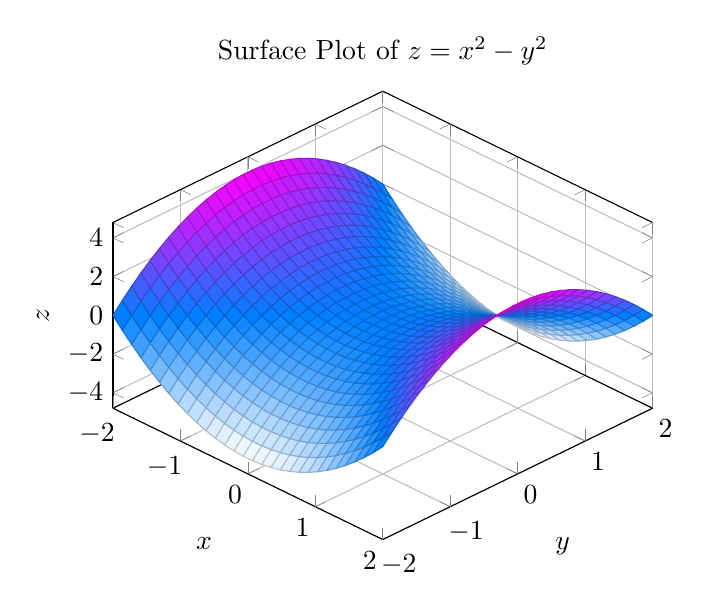
\begin{tikzpicture}
            \begin{axis}[
                view={45}{45},
                xlabel={$x$}, ylabel={$y$}, zlabel={$z$},
                colormap/cool,
                grid=major,
                domain=-2:2,
                y domain=-2:2,
                samples=30,
                z buffer=sort,
                title={Surface Plot of $z = x^2 - y^2$}
            ]
            \addplot3[surf] {x^2 - y^2};
            \end{axis}
        \end{tikzpicture}
    \end{minipage}%
    \hfill
    \begin{minipage}{0.4\textwidth}
        \centering
        \bigskip
        \begin{tabular}{ccc}
            \toprule
            \textbf{$x$} & \textbf{$y$} & \textbf{$z = x^2 - y^2$} \\
            \midrule
            -2 & -2 & 0 \\
            -1 & -1 & 0 \\
             0 &  0 & 0 \\
             1 &  1 & 0 \\
             2 &  2 & 0 \\
             2 &  0 & 4 \\
             0 &  2 & -4 \\
            \bottomrule
        \end{tabular}
    \end{minipage}
    \caption{\textit{Visualization of the function \( z = x^2 - y^2 \), showing the 3D surface plot and a table of input-output values.}}
    \label{fig:surface_table}
\end{figure}


\noindent The next figure demonstrates how plotting cross-sections simplifies understanding complex 3D surfaces. By combining slices with full 3D graphs, we can systematically analyze and interpret the behavior of functions of two variables. \\ \\ Below is a visualization of the function \( z = xy \), including a 3D surface plot and two 2D cross-sectional plots on the planes \( xz \) (at \( y=-1 \)) and \( yz \) (at \( x=1 \)).

\bigskip

\begin{figure}[H]
    \centering
    \begin{minipage}{0.55\textwidth}
        \centering
        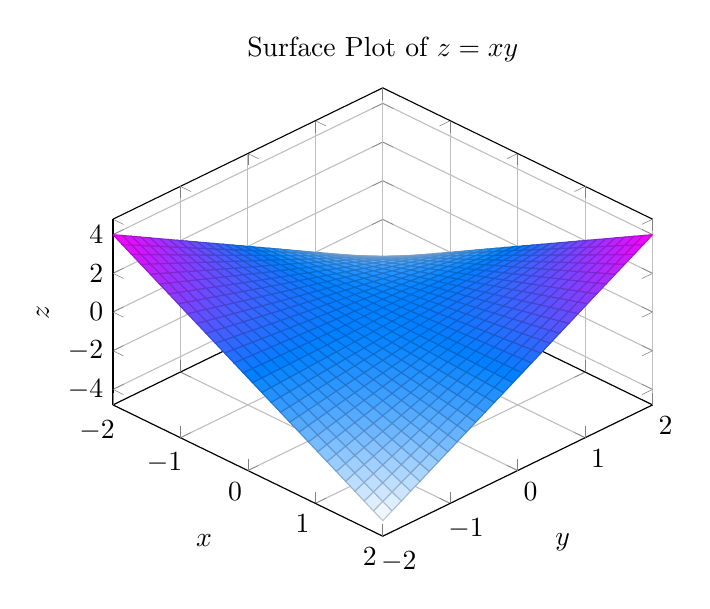
\begin{tikzpicture}
            \begin{axis}[
                view={45}{45},
                xlabel={$x$}, ylabel={$y$}, zlabel={$z$},
                colormap/cool,
                grid=major,
                domain=-2:2,
                y domain=-2:2,
                samples=30,
                z buffer=sort,
                title={Surface Plot of $z = xy$}
            ]
            \addplot3[surf] {x * y};
            \end{axis}
        \end{tikzpicture}
    \end{minipage}%
    \hfill
    \begin{minipage}{0.4\textwidth}
        \centering
        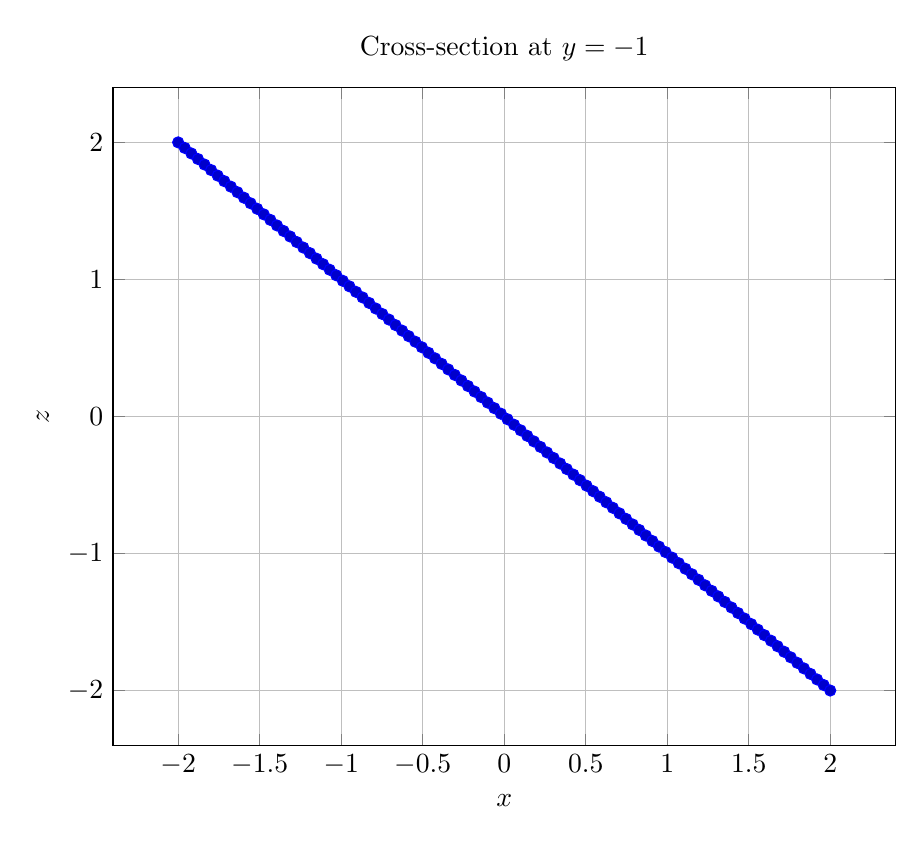
\begin{tikzpicture}
            \begin{axis}[
                xlabel={$x$}, ylabel={$z$},
                grid=major,
                domain=-2:2,
                samples=100,
                width=0.95\textwidth,
                title={Cross-section at $y = -1$}
            ]
            \addplot {-x};
            \end{axis}
        \end{tikzpicture}
\vspace{1.3em}
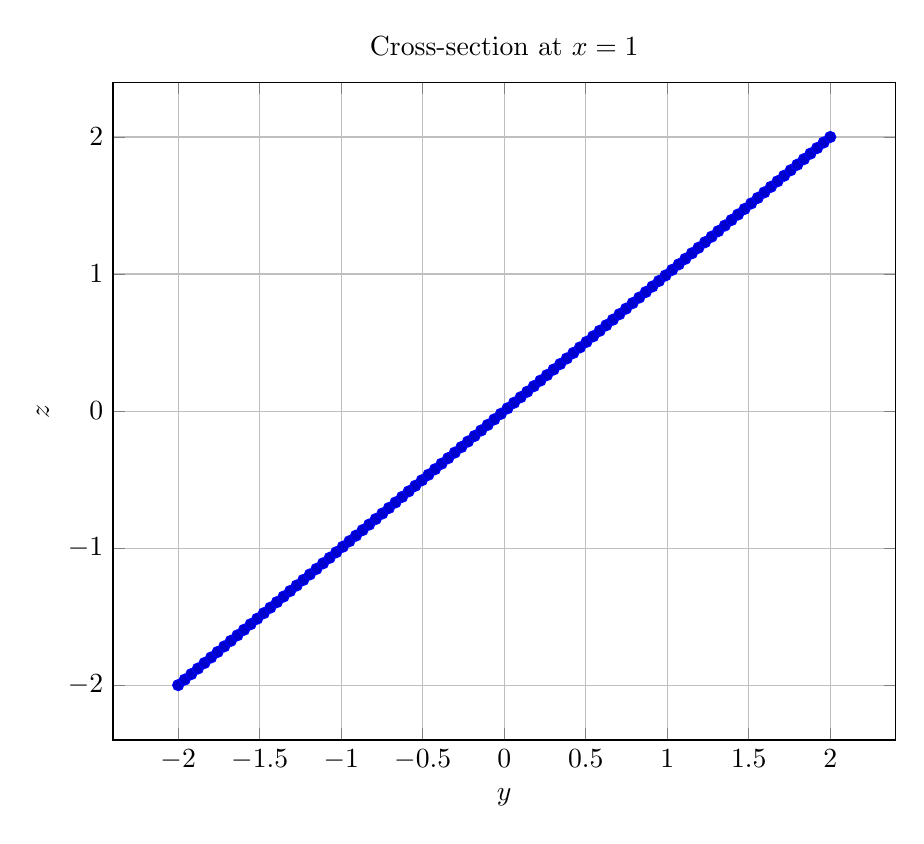
\begin{tikzpicture}
    \begin{axis}[
        xlabel={$y$}, ylabel={$z$},
        grid=major,
        domain=-2:2,
        samples=100,
        width=0.95\textwidth,
        title={Cross-section at $x = 1$}
    ]
    \addplot {x};
    \end{axis}
\end{tikzpicture}

    \end{minipage}
\caption{\textit{Visualization of the function \( z = x \cdot y \), showing the 3D surface plot alongside 2D cross-sections on the planes \( xz \) (at \( y=-1 \)) and \( yz \) (at \( x=1 \)).}}
    \label{fig:surface_cross_sections_new_example}
\end{figure}
\noindent We can see that by doing two 2D plots, we can reconstruct the plot visually with relative ease. In this particular example, it would be helpful to also see the case of $y=1$ to indicate the ``bend" in the 3D plot that we see. Just as you would spin an image around or a globe around to see all of its geometry, we essentially ``spin" the plot around by plotting different slices from difference planes. \\ \\ Let's take a look at an interesting applied example. The largest mountain in our solar system is Olympus Mons, located on Mars. One way to aid us in seeing the topology is to take cross sectional projections to see how this structure is formed. In fact, we know that Olympus Mons is a volcano in part because of the morphology and geological features obtained by such projections. In the picture below we slice two different sides of the mountain all the way through. Since the mountain is a volcano, we can especially see features such as the caldera much better using these slices.

\begin{figure}[H]
    \centering
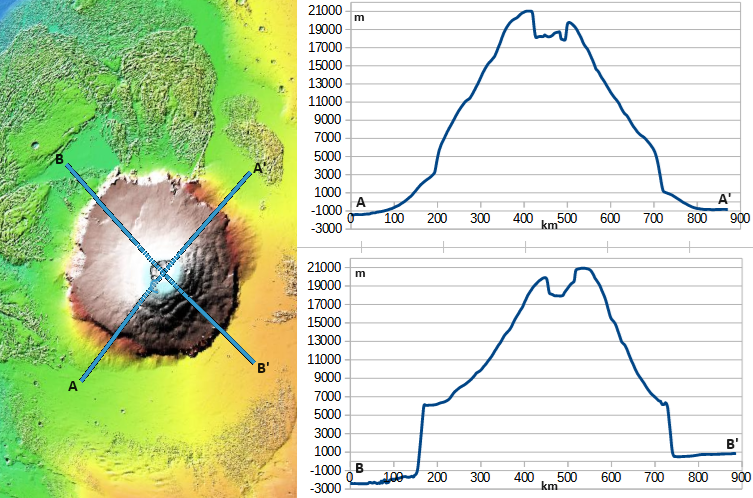
\includegraphics[width=.87\textwidth]{chapters/chp3_pics/Olympus_Mons_Elevation_Profiles.png}
\caption{\textit{Elevation profiles of Olympus Mons along SW-to-NE and NW-to-SE transects across the mountain. Image from Wikipedia}}
    \label{fig:olympus_mons}
\end{figure}




\subsubsection*{Level Curves} \index{Level Curves}

\noindent Level curves of a function \( f(x, y) \) are the set of points in the \( xy \)-plane where the function takes on a constant value \( k \), expressed by the equation \( f(x, y) = k \). By plotting these curves for various values of \( k \), we can visualize the function in two dimensions, gaining insights into its behavior without needing to represent the full three-dimensional surface. You may have even seen these types of plots on geographic plots. These are yet another tool that aid in understanding the shape of the terrain and identifying features like hills and valleys.

    \begin{figure}[H]
        \centering
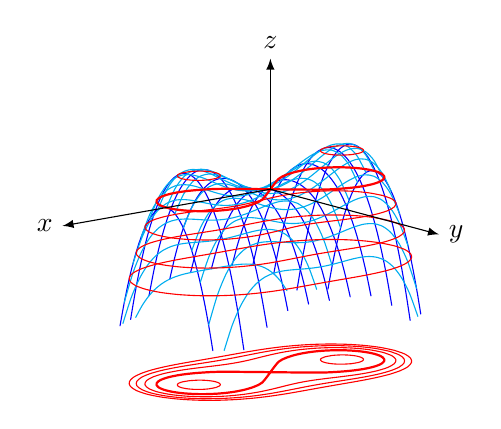
\begin{tikzpicture}[scale=1.7,line cap=round,line join=round,
   x={(-0.7766cm,-0.1369cm)},y={(0.6300cm,-0.1688cm)},z={(0cm,0.9761cm)}]
\def\xmin{1}
\def\ymin{0.7}
\pgfmathsetmacro\xstep{\xmin-0.2}
\pgfmathsetmacro\ystep{\ymin-0.1}
\def\h{-1.4} % projection height
% blue lines, sections perpendicular to the x axis
\foreach\i in{-\xmin,-\xstep,...,\xmin}
{%                 domain in which z>=-1
  \pgfmathsetmacro\xdom{min(\ymin,sqrt(-0.5-\i*\i+0.5*sqrt(5+8*\i*\i)))}
  \draw[blue] plot[domain=-\xdom:\xdom,samples=25,smooth]
    (\i,\x,{-(\i*\i+\x*\x)*(\i*\i+\x*\x)+(\i*\i-\x*\x)});
}
% cyan lines, sections perpendicular to the y axis
\foreach\i in{-\ymin,-\ystep,...,\ymin}
{%                 domain in which z>=-1
  \pgfmathsetmacro\xdom{min(\xmin,sqrt(0.5-\i*\i+0.5*sqrt(5-8*\i*\i)))} 
  \draw[cyan] plot[domain=-\xdom:\xdom,samples=25,smooth]
    (\x,\i,{-(\x*\x+\i*\i)*(\x*\x+\i*\i)+(\x*\x-\i*\i)});
}
% Bernouilli's lemniscate (and projection)
\foreach\a in {0,180} \foreach\z in {0,\h}
{%
  \draw[thick,red] plot[domain=-45+\a: 45+\a,samples=25,smooth]
    ({sqrt(cos(2*\x))*cos(\x)},{sqrt(cos(2*\x))*sin(\x)},\z);
}
% Other level curves (and projections)
\def\z{0.2}
\pgfmathsetmacro\xdom{0.5*acos(2*sqrt(\z))-0.005} % precission problem, I think
\foreach\zz in {\z,\h} \foreach\a in {0,180} \foreach\s in {-1,1}
{%
  \draw[red] plot[domain=\a-\xdom:\a+\xdom,samples=25,smooth]
    ({sqrt(0.5*cos(2*\x)+0.5*\s*sqrt(cos(2*\x)*cos(2*\x)-4*\z))*cos(\x)},
     {sqrt(0.5*cos(2*\x)+0.5*\s*sqrt(cos(2*\x)*cos(2*\x)-4*\z))*sin(\x)},\zz);
}
\foreach\z in {-0.2,-0.4,-0.6} \foreach\zz in {\z,\h}
{%
  \draw[red] plot[domain=-180:180,samples=51,smooth]
   ({sqrt(0.5*cos(2*\x)+0.5*sqrt(cos(2*\x)*cos(2*\x)-4*\z))*cos(\x)},
    {sqrt(0.5*cos(2*\x)+0.5*sqrt(cos(2*\x)*cos(2*\x)-4*\z))*sin(\x)},\zz);
}
% axes
\draw[-latex] (0,0,0) -- (2,0,0) node[left]  {$x$};
\draw[-latex] (0,0,0) -- (0,2,0) node[right] {$y$};
\draw[-latex] (0,0,0) -- (0,0,1) node[above] {$z$};
\end{tikzpicture}
\caption{\textit{A 3D surface with its level curves projected below, including the Bernoulli lemniscate (the infinity shaped level curve)}}
\end{figure}


\noindent Now that we have a basic understanding of what level curves are and why they are useful, let's explore the process of plotting them in more detail. Level curves provide a two-dimensional representation of a function of two variables by showing all points \( (x, y) \) where the function takes on the same value \( k \). This visualization is particularly helpful for understanding the behavior of multivariable functions without requiring a full 3D plot. Here's how to systematically plot level curves step by step:

\begin{enumerate}
    \item \textbf{Select Values of \( k \):} Choose several constant values for \( k \) that capture the key features of the function. It's important to select a range of \( k \) values—both positive and negative, if applicable—to represent the function's full behavior. For functions with periodic or oscillatory behavior, ensure the \( k \)-values align with significant points such as peaks, troughs, and zeros.

    \item \textbf{Set \( f(x, y) = k \):} For each chosen value of \( k \), substitute it into the function \( f(x, y) \) to define the corresponding level curve. This equation represents all points \( (x, y) \) where the function equals \( k \).

    \item \textbf{Solve for One Variable in Terms of the Other:} Rearrange the equation \( f(x, y) = k \) to express \( y \) as a function of \( x \), or \( x \) as a function of \( y \), if possible. For example, in circular or radial symmetry, the equation might simplify to an expression for \( r^2 = x^2 + y^2 \). For more complex functions, this step may involve approximations or parametric forms.

    \item \textbf{Plot Each Level Curve:} Using the equations derived, carefully plot the curves on the \( xy \)-plane. For simple equations, this can be done by hand. For more intricate equations, consider using graphing tools or software to ensure accuracy. Ensure that each curve is plotted with sufficient points to capture its shape.

    \item \textbf{Label the Curves:} Clearly label each curve with its corresponding \( k \)-value. This can be done directly on the graph or through a legend. For enhanced clarity, consider using color coding to visually differentiate the curves based on their \( k \)-values.

    \item \textbf{Analyze the Overall Behavior:} Once the level curves are plotted, examine their spacing and patterns. For instance, closely spaced curves indicate regions of rapid change in the function, while widely spaced curves suggest more gradual variation. This step helps in interpreting the nature of the function and its gradients.
\end{enumerate}

\exampleline
\begin{example}
Consider the function \( z = \sin(x^2 + y^2) \) defined for all \( (x, y) \in \mathbb{R}^2 \).

\begin{enumerate}
    \item Plot the graph of \( z = \sin(x^2 + y^2) \) as a surface in 3D space.
    \item Plot the level curves of \( z = \sin(x^2 + y^2) \) for selected \( z \)-values computed by hand.
\end{enumerate}

\begin{solution}
\begin{enumerate}
    \item The graph of \( z = \sin(x^2 + y^2) \) exhibits circular symmetry. Recall that
    \[
    \begin{aligned}
    \sin(\theta) = 1 &\quad \text{if} \quad \theta = \frac{\pi}{2}+2\pi n,\\[6pt]
    \sin(\theta) = -1 &\quad \text{if} \quad \theta = -\frac{\pi}{2}+2\pi n,\\[6pt]
    \sin(\theta) = 0 &\quad \text{if} \quad \theta = \pi n,
    \end{aligned}
    \]
    for any integer \( n \). Since \( \theta = x^2+y^2 \), the peaks (\( z=1 \)) occur when
    \[
    x^2+y^2 = \frac{\pi}{2}+2\pi n,
    \]
    the troughs (\( z=-1 \)) when
    \[
    x^2+y^2 = -\frac{\pi}{2}+2\pi n,
    \]
    and the zeros (\( z=0 \)) when
    \[
    x^2+y^2 = \pi n.
    \]

    \begin{figure}[H]
        \centering
        \resizebox{0.55\textwidth}{!}{%
            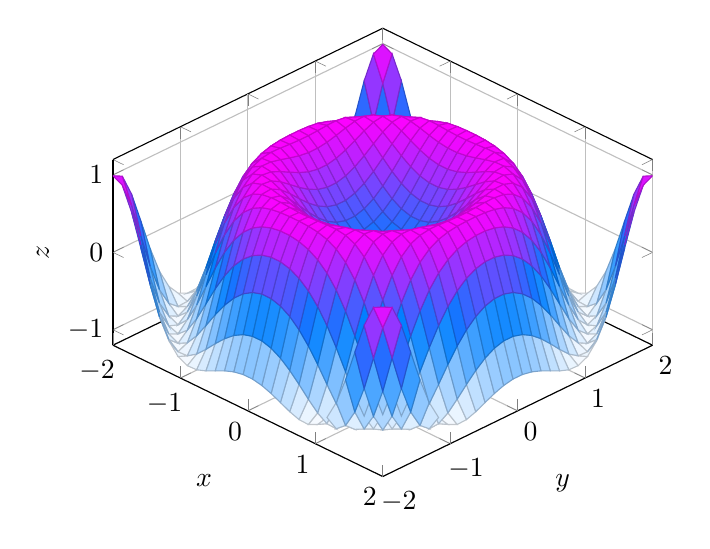
\begin{tikzpicture}
                \begin{axis}[
                    view={45}{45},
                    xlabel={$x$}, ylabel={$y$}, zlabel={$z$},
                    colormap/cool,
                    grid=major,
                    domain=-2:2,
                    y domain=-2:2,
                    samples=30,
                    z buffer=sort
                ]
                \addplot3[surf] {sin(deg(x^2 + y^2))};
                \end{axis}
            \end{tikzpicture}
        }
        \caption{\textit{Graph of \( z = \sin(x^2+y^2) \), a sinusoidal surface.}}
        \label{fig:surface_sin_x2y2}
    \end{figure}

    \item To draw the level curves, we set \( \sin(x^2+y^2)=k \) for specific \( k \)-values. This gives:
    \begin{itemize}
        \item \textbf{For \( z=1 \):} Solve 
        \[
        x^2+y^2 = \frac{\pi}{2}+2\pi n \quad \Longrightarrow \quad r = \sqrt{\frac{\pi}{2}+2\pi n}.
        \]
        For example,
        \[
        \begin{aligned}
        n=0:\quad r &= \sqrt{\frac{\pi}{2}} \approx 1.25,\\[6pt]
        n=1:\quad r &= \sqrt{\frac{5\pi}{2}} \approx 2.80
        \end{aligned}
        \]
        
        \item \textbf{For \( z=-1 \):} Solve 
        \[
        x^2+y^2 = -\frac{\pi}{2}+2\pi n \quad (n \geq 1) \quad \Longrightarrow \quad r = \sqrt{-\frac{\pi}{2}+2\pi n}.
        \]
        For example,
        \[
        \begin{aligned}
        n=1:\quad r &= \sqrt{\frac{3\pi}{2}} \approx 2.17,\\[6pt]
        n=2:\quad r &= \sqrt{\frac{7\pi}{2}} \approx 3.32
        \end{aligned}
        \]
        
        \item \textbf{For \( z=0 \):} Solve 
        \[
        x^2+y^2 = \pi n \quad \Longrightarrow \quad r = \sqrt{\pi n}.
        \]
        For example,
        \[
        \begin{aligned}
        n=1:\quad r &= \sqrt{\pi} \approx 1.77,\\[6pt]
        n=2:\quad r &= \sqrt{2\pi} \approx 2.51
        \end{aligned}
        \]
    \end{itemize}

\begin{figure}[H]
    \centering
    \begin{tikzpicture}[scale=0.35]
        % Axes
        \draw[->] (-9,0) -- (9,0) node[anchor=north] {$x$};
        \draw[->] (0,-9) -- (0,9) node[anchor=west] {$y$};

        % Level curves for z=1 (blue)
        \draw[blue, thick] (0,0) circle (1.25);
        \draw[blue, thick] (0,0) circle (2.80);
        \draw[blue, thick] (0,0) circle (3.76);
        \draw[blue, thick] (0,0) circle (4.52);

        % Level curves for z=-1 (red)
        \draw[red, thick] (0,0) circle (2.17);
        \draw[red, thick] (0,0) circle (3.32);
        \draw[red, thick] (0,0) circle (4.16);
        \draw[red, thick] (0,0) circle (4.86);

        % Level curves for z=0 (green)
        \draw[green, thick] (0,0) circle (1.77);
        \draw[green, thick] (0,0) circle (2.51);
        \draw[green, thick] (0,0) circle (3.07);
        \draw[green, thick] (0,0) circle (3.54);

        % Legend
        \node[draw=none, fill=none, anchor=north west] at (10,6) {
            \begin{tikzpicture}
                \draw[blue, thick] (0,0) -- (1,0) node[anchor=west] {$z=1$};
                \draw[red, thick] (0,-0.5) -- (1,-0.5) node[anchor=west] {$z=-1$};
                \draw[green, thick] (0,-1) -- (1,-1) node[anchor=west] {$z=0$};
            \end{tikzpicture}
        };
    \end{tikzpicture}
    \caption{\textit{Level curves for \( z = \sin(x^2+y^2) \) with additional rings.}}
\end{figure}

\end{enumerate}
\end{solution}
\end{example}

\exampleline
\begin{example}
Consider the function \( z = \cos(y) \) defined for all \( (x, y) \in \mathbb{R}^2 \).

\begin{enumerate}
    \item Plot the graph of \( z = \cos(y) \) as a surface in 3D space.
    \item Plot the level curves of \( z = \cos(y) \) for selected \( z \)-values computed by hand.
\end{enumerate}

\begin{solution}
\begin{enumerate}
    \item The graph of \( z = \cos(y) \) represents a cosine wave in the \( y \)-direction that is extruded along the \( x \)-axis. As \( y \) varies, \( z \) oscillates between \(-1\) and \(1\).

    \begin{figure}[H]
        \centering
        \resizebox{0.55\textwidth}{!}{%
            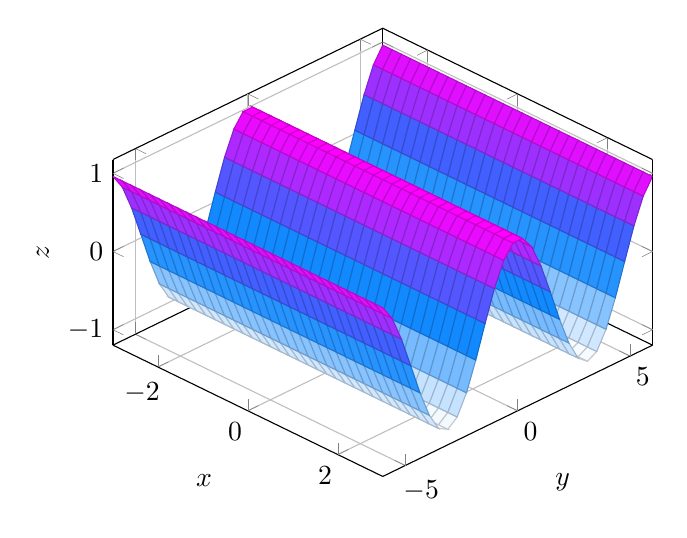
\begin{tikzpicture}
                \begin{axis}[
                    view={45}{45},
                    xlabel={$x$}, ylabel={$y$}, zlabel={$z$},
                    colormap/cool,
                    grid=major,
                    domain=-3:3,
                    y domain=-6:6,
                    samples=30,
                    z buffer=sort
                ]
                \addplot3[surf] {cos(deg(y))};
                \end{axis}
            \end{tikzpicture}
        }
        \caption{\textit{Graph of \( z = \cos(y) \), a cosine wave surface extruded along \( x \).}}
        \label{fig:surface_cos_y}
    \end{figure}

    \item To find the level curves, we set \( \cos(y)=k \) for specific values of \( k \) (with \( -1 \le k \le 1 \)). The general solutions for \( y \) are:
    \[
    \begin{aligned}
    \cos(y) = 1 \quad &\Longrightarrow \quad y = 0 + 2\pi n,\\[6pt]
    \cos(y) = -1 \quad &\Longrightarrow \quad y = \pi + 2\pi n,\\[6pt]
    \cos(y) = 0 \quad &\Longrightarrow \quad y = \frac{\pi}{2} + \pi n,
    \end{aligned}
    \]
    where \( n \) is any integer. For a few specific level curves, we choose:
    \begin{itemize}
        \item \textbf{\( z=1 \):} \( y = 0,\, 2\pi,\, -2\pi,\, \ldots \)
        \item \textbf{\( z=-1 \):} \( y = \pi,\, -\pi,\, 3\pi,\, \ldots \)
        \item \textbf{\( z=0 \):} \( y = \frac{\pi}{2},\, -\frac{\pi}{2},\, \frac{3\pi}{2},\, \ldots \)
    \end{itemize}
    Since \( x \) is unrestricted, the level curves in the \( xy \)-plane are horizontal lines at these \( y \)-values.

    \begin{figure}[H]
        \centering
        \begin{tikzpicture}[scale=0.5]
            % Draw axes
            \draw[->] (-5,0) -- (5,0) node[anchor=north] {$x$};
            \draw[->] (0,-4) -- (0,4) node[anchor=east] {$y$};
            
            % Level curve for z=1 (blue): y = 0
            \draw[blue, thick] (-5,0) -- (5,0);
            
            % Level curves for z=-1 (red): y = π and y = -π
            \draw[red, thick] (-5,3.14) -- (5,3.14);
            \draw[red, thick] (-5,-3.14) -- (5,-3.14);
            
            % Level curves for z=0 (green): y = π/2 and y = -π/2
            \draw[green, thick] (-5,1.57) -- (5,1.57);
            \draw[green, thick] (-5,-1.57) -- (5,-1.57);
            
            % Legend
            \node[draw=none, fill=none, anchor=north west] at (6,3) {
                \begin{tikzpicture}[scale=0.8]
                    \draw[blue, thick] (0,0) -- (1,0) node[anchor=west] {$z=1$};
                    \draw[red, thick] (0,-0.5) -- (1,-0.5) node[anchor=west] {$z=-1$};
                    \draw[green, thick] (0,-1) -- (1,-1) node[anchor=west] {$z=0$};
                \end{tikzpicture}
            };
        \end{tikzpicture}
        \caption{\textit{Level curves for \( z = \cos(y) \) in the \( xy \)-plane.}}
    \end{figure}
\end{enumerate}
\end{solution}
\end{example}
\exampleline




\subsubsection*{Common 3D Equations}
\noindent As is the case in single-variable mathematics, we can depend on familiar examples to help make sense of functions on sight.

\begin{itemize}
    \item \textbf{Quadric Surfaces:} Paraboloids, hyperboloids, and ellipsoids are common surfaces that can often be graphed as functions of \( x \) and \( y \). These surfaces are studied in more detail in Lecture 1.5. Examples include:
    \begin{itemize}
        \item Paraboloid: \( z = x^2 + y^2 \)
        \item Hyperboloid of One Sheet: \( x^2 + y^2 - z^2 = 1 \)
        \item Ellipsoid: \( \frac{x^2}{a^2} + \frac{y^2}{b^2} + \frac{z^2}{c^2} = 1 \)
    \end{itemize}
    
    \item \textbf{Sphere:} A sphere represents a special case of an ellipsoid where all axes are equal. The equation is: 
    \[
    x^2 + y^2 + z^2 = r^2
    \]
    
    \item \textbf{Plane:} A plane can be described as a linear function in three variables. For example:
    \[
    z = ax + by + c
    \]
    
    \item \textbf{Cylinder:} Cylinders are surfaces generated by extending a curve along a straight line parallel to an axis. Examples include:
    \begin{itemize}
        \item Circular Cylinder: \( x^2 + y^2 = r^2 \)
        \item Parabolic Cylinder: \( z = x^2 \)
    \end{itemize}
    
    \item \textbf{Cone:} A cone is a surface that extends a curve in a way that all points of the curve are connected to a single vertex. For example:
    \[
    z^2 = x^2 + y^2
    \]
\end{itemize}

\subsection*{Functions of Three or More Variables} \index{Functions of Three or More Variables}

\noindent A function of three variables assigns a real number \( w = f(x, y, z) \) to each point \( (x, y, z) \) within a subset of \( \mathbb{R}^3 \). The challenge in working with such functions lies in the fact that their graphs exist in four-dimensional space, a realm beyond our ability to visualize directly. Unlike the graph of a function of one variable, which forms a curve in \( \mathbb{R}^2 \), or a function of two variables, which forms a surface in \( \mathbb{R}^3 \), the graph of \( f(x, y, z) \) resists geometric representation. Despite this limitation, a variety of powerful techniques enable us to analyze and understand these functions with clarity and precision. Specifically, the most comprehensive way that I can think about it is by the analogy of a three-dimensional shadow: a shadow reduces a 3D object down to 2D, therefore a 3D object is the shadow of a 4D object. This means that projections will be our greatest ally. \\

\noindent To streamline notation for functions of multiple variables, it is common to represent the input \( (x, y, z) \) as a single entity, often written as \( \mathbf{x} \). This allows us to express \( f(x, y, z) \) in a more concise form:
\[
f(\mathbf{x}),
\]
where \( \mathbf{x} \) represents the vector of input variables:
\[
\mathbf{x} = (x, y, z).
\]
This notation generalizes naturally to functions of \( n \) variables, where \( \mathbf{x} = (x_1, x_2, \ldots, x_n) \) is a vector in \( \mathbb{R}^n \). To emphasize the structure of the input variables, we can further represent \( \mathbf{x} \) as a column vector:
\[
\mathbf{x} = 
\begin{bmatrix}
x \\ 
y \\ 
z
\end{bmatrix}.
\]
With this notation, the function \( f(x, y, z) \) becomes \( f(\mathbf{x}) \), where \( \mathbf{x} \) is the input vector. Alternatively, we can express \( \mathbf{x} \) explicitly as a column vector:
\[
f(\mathbf{x}) = f\left(\begin{bmatrix} x \\ y \\ z \end{bmatrix}\right),
\]
providing a unified framework for analyzing functions of several variables. For instance, a temperature field \( T \) in three-dimensional space can be expressed as:
\[
T = f(\mathbf{t}) = f\left(\begin{bmatrix} t_x \\ t_y \\ t_z \end{bmatrix}\right) =  f(t_x,t_y,t_z) = t_x^2 + t_y^2 + t_z^2
\]
where \( \mathbf{t} \) represents a point in \( \mathbb{R}^3 \). This column vector-based notation is particularly valuable in advanced topics like gradients, divergence, and vector-valued functions, as it simplifies both expression and computation.




\subsubsection*{Graphs and Visualization}

\noindent While we cannot graph functions of three variables directly in three-dimensional space, we can understand them through level surfaces and projections. A \textbf{level surface} is the set of all points \((x, y, z)\) in the domain of \(f(x, y, z)\) where the function takes a constant value, \( w = k \). These surfaces are three-dimensional analogues of level curves for functions of two variables. For example, fixing \( w = 0 \), the level surface \( f(x, y, z) = 0 \) provides a snapshot of the function's behavior in three-dimensional space. \\

\noindent The idea is analogous to projections, where we imagine the three-dimensional representation of a function as the ``shadow" of its four-dimensional graph. By holding one variable constant, such as \( z = 0 \), we reduce the function to \( w = f(x, y, 0) \), which can be plotted as a surface in three-dimensional space. Repeating this process for various fixed values of \( z \) (or any other variable) gives a series of surfaces that collectively reveal the structure of the original function. This approach bridges the gap between our spatial intuition and the abstraction of higher-dimensional spaces.

\subsubsection*{Level Surfaces} \index{Level Surfaces}

\noindent Plotting a level surface will be very similar to our level curves. Let's take a look at a sphere \(f(x, y, z) = x^2 + y^2 + z^2\). The level surfaces are determined by solving:
\[
f(x, y, z) = k \implies x^2 + y^2 + z^2 = k.
\]

\noindent For different values of \( k \), the level surfaces represent spheres centered at the origin with radius \(\sqrt{k}\):
\begin{itemize}
    \item \( k = 1 \): Sphere of radius 1.
    \item \( k = 4 \): Sphere of radius 2.
    \item \( k = 9 \): Sphere of radius 3.
\end{itemize}

\noindent To visualize these level surfaces, we plot the spheres for \( k = 1, 4, 9 \). The surfaces demonstrate the isotropic nature of the function \( f(x, y, z) \), where the value of \( w \) depends only on the distance from the origin.

\begin{figure}[H]
    \centering
    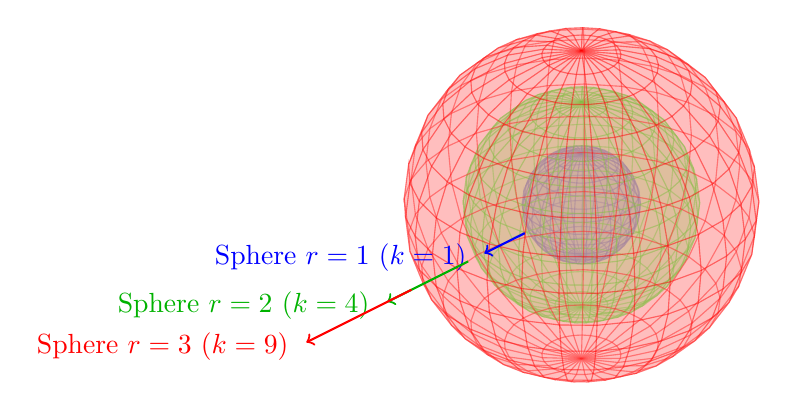
\begin{tikzpicture}
        \begin{axis}[
            view={60}{30},
            axis equal image,
            hide axis,
            width=12cm,
            height=12cm,
            xmin=-4, xmax=4,
            ymin=-4, ymax=4,
            zmin=-4, zmax=4,
            clip=false, % Prevent clipping of callouts
        ]
            % Sphere of radius 1 (k=1)
            \addplot3[
                surf,
                shader=flat,
                opacity=0.3,
                samples=30,
                samples y=15,
                domain=0:360,
                y domain=0:180,
                z buffer=sort,
                fill=blue!50,
                draw=blue,
            ]
            ({1*cos(x)*sin(y)},
             {1*sin(x)*sin(y)},
             {1*cos(y)});
             
            % Sphere of radius 2 (k=4)
            \addplot3[
                surf,
                shader=flat,
                opacity=0.3,
                samples=30,
                samples y=15,
                domain=0:360,
                y domain=0:180,
                z buffer=sort,
                fill=green!50,
                draw=green,
            ]
            ({2*cos(x)*sin(y)},
             {2*sin(x)*sin(y)},
             {2*cos(y)});
             
            % Sphere of radius 3 (k=9)
            \addplot3[
                surf,
                shader=flat,
                opacity=0.3,
                samples=30,
                samples y=15,
                domain=0:360,
                y domain=0:180,
                z buffer=sort,
                fill=red!50,
                draw=red,
            ]
            ({3*cos(x)*sin(y)},
             {3*sin(x)*sin(y)},
             {3*cos(y)});
             
            % Callout for Sphere of radius 1 (k=1)
            \draw[->, thick, blue] (axis cs: -0.7, -0.7, -0.7) -- (axis cs: -1.2, -1.2, -1.2);
            \node[anchor=east, blue] at (axis cs: -1.3, -1.3, -1.3) {Sphere \( r = 1 \) ($k=1$)};
            
            % Callout for Sphere of radius 2 (k=4)
            \draw[->, thick, green!70!black] (axis cs: -1.4, -1.4, -1.4) -- (axis cs: -2.4, -2.4, -2.4);
            \node[anchor=east, green!70!black] at (axis cs: -2.5, -2.5, -2.5) {Sphere \( r = 2 \) ($k=4$)};
            
            % Callout for Sphere of radius 3 (k=9)
            \draw[->, thick, red] (axis cs: -2.1, -2.1, -2.1) -- (axis cs: -3.4, -3.4, -3.4);
            \node[anchor=east, red] at (axis cs: -3.5, -3.5, -3.5) {Sphere \( r = 3 \) ($k=9$)};
        \end{axis}
    \end{tikzpicture}
    \caption{\textit{Level surfaces of \( f(x, y, z) = x^2 + y^2 + z^2 = k\) for \( k = 1, 4, 9 \), represented as concentric spheres}}
    \label{fig:level_surfaces_example}
\end{figure}

\noindent While this doesn't exactly paint the complete picture, you may begin to see how hypergeometry works. Perhaps you have seen a hypercube represented before but not sure why it looks like it does. With level surfaces it may begin to make more sense:


\begin{figure}[H]
    \centering
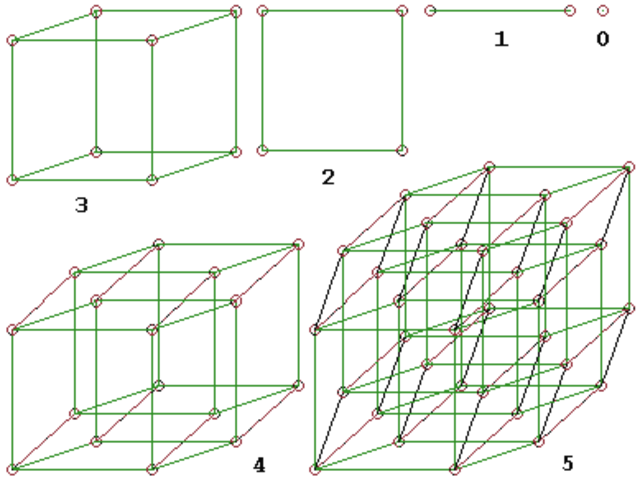
\includegraphics[width=.5\textwidth]{chapters/chp3_pics/hypercube.png}
\caption{\textit{Cubes of dimensions 1 through 5. Above three dimensions, these are often called hypercubes, or $n$-cubes. Image from Wikipedia}}
    \label{fig:4d_cube}
\end{figure}
%https://commons.wikimedia.org/wiki/File:WUERFEL5_0-_bis_5-dimensionale_Wuerfelanaloge.png
\subsection*{Visualizing Functions of Several Variables}

\noindent As the number of variables in a function increases, direct visualization becomes increasingly challenging. For functions of two or three variables, graphs and level sets provide intuitive insights. However, for functions involving more than three variables, such as \( f(x_1, x_2, \ldots, x_n) \), we rely on abstract representations, projections, and numerical tools to understand their behavior.

\paragraph{Higher-Dimensional Analogues:} In higher dimensions, familiar geometric objects like lines, planes, and spheres generalize:
\begin{itemize}
    \item A \textbf{hyperplane} in \( \mathbb{R}^n \) is defined by a linear equation, such as \( a_1x_1 + a_2x_2 + \cdots + a_nx_n = c \). It is the \( n \)-dimensional analogue of a plane in \( \mathbb{R}^3 \).
    \item A \textbf{hypersphere} in \( \mathbb{R}^n \) is defined by \( x_1^2 + x_2^2 + \cdots + x_n^2 = r^2 \). In \( \mathbb{R}^4 \), for example, this represents the set of points equidistant from a center, analogous to a sphere in \( \mathbb{R}^3 \).
\end{itemize}

\paragraph{Applications in Machine Learning:} \index{Machine Learning} Functions of several variables are fundamental in machine learning, particularly in classification tasks. For instance:
\begin{itemize}
    \item \textbf{Hyperplanes in Classification:} In supervised learning, hyperplanes are often used to separate data points belonging to different classes. For example, a linear classifier uses a hyperplane to divide the feature space into regions corresponding to different categories.
    \item \textbf{Support Vector Machines (SVMs):} SVMs are powerful classification algorithms that construct an optimal hyperplane to maximize the margin between data points of different classes. Mathematically, the hyperplane is defined as:
    \[
    \mathbf{w} \cdot \mathbf{x} - b = 0,
    \]
    where \( \mathbf{w} \) is the weight vector, \( \mathbf{x} \) is a data point, and \( b \) is a bias term. The margin is maximized by solving an optimization problem involving the constraint:
    \[
    y_i (\mathbf{w} \cdot \mathbf{x}_i - b) \geq 1,
    \]
    where \( y_i \) represents the class label of \( \mathbf{x}_i \).
\end{itemize}


\begin{figure}[H]
    \centering
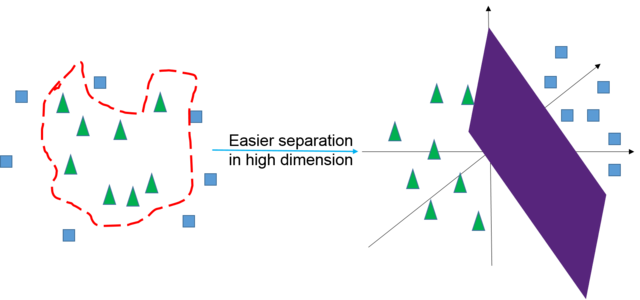
\includegraphics[width=.7\textwidth]{chapters/chp3_pics/Supporting_Vector_Machine.png}
\caption{\textit{Hyperplanes used for optimal classification in SVMs. Image from Wikipedia}}
    \label{fig:svm}
\end{figure}
%https://commons.wikimedia.org/wiki/File:Supporting_Vector_Machine.png

\noindent Although these applications arise in higher dimensions, the underlying concepts of hyperplanes and optimization are rooted in multivariable calculus.



\newpage


\lecture{Limits and Continuity} \index{Limits and Continuity}

\noindent In single-variable calculus, the concepts of limits and continuity form the foundation for understanding the behavior of functions near points of interest and for establishing the differentiability and integrability of functions. In multivariable calculus, these ideas extend naturally but require a more nuanced treatment due to the increased complexity introduced by multiple independent variables. This lecture delves into the concepts of limits and continuity in the context of multivariable functions, exploring their definitions, properties, and challenges.

\subsection*{Limits in Higher Dimensions}

\noindent The concept of a limit is a cornerstone of calculus and extends naturally to functions of several variables. However, understanding this extension requires a thoughtful approach, as the introduction of additional variables adds layers of complexity. \\ \\ In single-variable calculus, we define the limit \( \lim_{x \to a} f(x) = L \) as the value \( L \) that \( f(x) \) approaches as \( x \) gets arbitrarily close to \( a \). For multivariable functions, the same principle applies, but now the input \( (x, y) \) can approach a target point \( (a, b) \) from infinitely many directions in the plane. This distinction is key: in one dimension, there are only two possible approaches to \( a \) (from the left or right), whereas in two dimensions, there are infinitely many paths. 

\begin{figure}[H]
    \centering
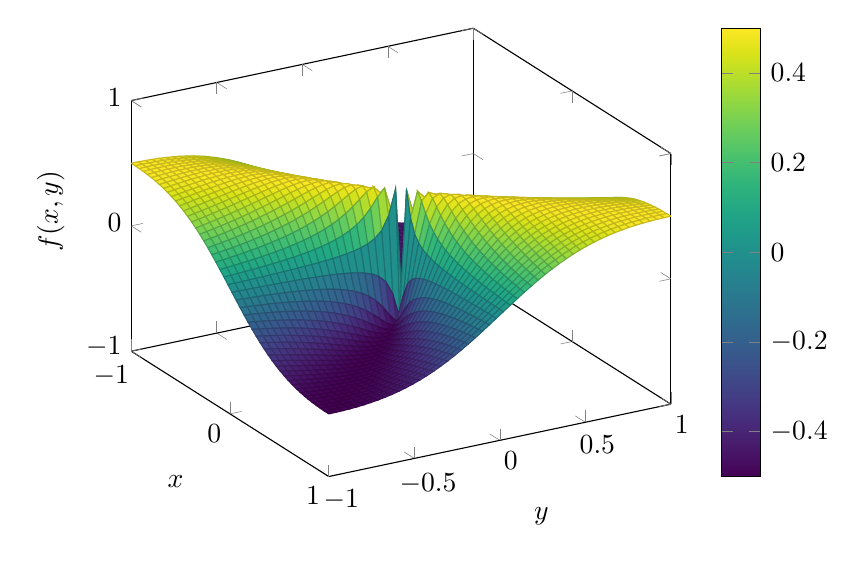
\begin{tikzpicture}
\begin{axis}[
    view={60}{30},
    xlabel={$x$},
    ylabel={$y$},
    zlabel={$f(x, y)$},
    domain=-1:1,
    y domain=-1:1,
    samples=50,
    samples y=50,
    zmin=-1,
    zmax=1,
    colorbar,
    colormap/viridis,
]
\addplot3[surf] {x*y/(x^2 + y^2)};
\end{axis}
\end{tikzpicture}
    \caption{\textit{Graph of \(z = \frac{x y}{x^2 + y^2} \), where the limit does not exist at $(0,0)$}}
    \label{fig:surface_xy_over_x2y2}
\end{figure}


\noindent To understand limits intuitively, imagine the behavior of a function \( f(x, y) \) as you move closer and closer to a fixed point \( (a, b) \). The value of \( f(x, y) \) should stabilize and become arbitrarily close to a specific number \( L \), regardless of the path taken. If the value of \( f(x, y) \) changes depending on the path, the limit does not exist.

\subsubsection*{Properties of Multivariable Limits} \index{Multivariable Limits}

\noindent Before diving into techniques for evaluating limits, it is helpful to understand some basic properties that govern multivariable limits. These properties, analogous to their single-variable counterparts, provide useful shortcuts and insights into the behavior of multivariable functions as they approach a limit.

\begin{itemize}
    \item \textbf{Linearity:} If \( \lim_{(x, y) \to (a, b)} f(x, y) = L \) and \( \lim_{(x, y) \to (a, b)} g(x, y) = M \), then for any constants \( c_1 \) and \( c_2 \):
    \[
    \lim_{(x, y) \to (a, b)} \left[ c_1 f(x, y) + c_2 g(x, y) \right] = c_1 L + c_2 M.
    \]

    \item \textbf{Product Rule:} If \( \lim_{(x, y) \to (a, b)} f(x, y) = L \) and \( \lim_{(x, y) \to (a, b)} g(x, y) = M \), then:
    \[
    \lim_{(x, y) \to (a, b)} \left[ f(x, y) g(x, y) \right] = L \cdot M.
    \]

    \item \textbf{Quotient Rule:} If \( \lim_{(x, y) \to (a, b)} f(x, y) = L \) and \( \lim_{(x, y) \to (a, b)} g(x, y) = M \), with \( M \neq 0 \), then:
    \[
    \lim_{(x, y) \to (a, b)} \frac{f(x, y)}{g(x, y)} = \frac{L}{M}.
    \]

    \item \textbf{Composition Rule:} If \( \lim_{(x, y) \to (a, b)} f(x, y) = L \) and \( \lim_{z \to L} g(z) = N \), where \( g \) is continuous at \( L \), then:
    \[
    \lim_{(x, y) \to (a, b)} g(f(x, y)) = g(L).
    \]

    \item \textbf{Limits of Polynomials and Rational Functions:} For polynomial functions \( f(x, y) \) and \( g(x, y) \), the limit as \( (x, y) \to (a, b) \) can often be found by direct substitution:
    \[
    \lim_{(x, y) \to (a, b)} f(x, y) = f(a, b).
    \]
    For rational functions \( f(x, y)/g(x, y) \), this holds as long as \( g(a, b) \neq 0 \).

    \item \textbf{Continuity and Limits:} If \( f(x, y) \) is continuous at \( (a, b) \), then the limit as \( (x, y) \to (a, b) \) is simply the value of the function at that point:
    \[
    \lim_{(x, y) \to (a, b)} f(x, y) = f(a, b).
    \]
\end{itemize}

\noindent These properties simplify the evaluation of many limits and help identify when more advanced techniques, such as polar coordinates or path dependence analysis, may be necessary. Combined with the techniques described in the following section, they form the backbone of solving multivariable limit problems.

\subsubsection*{Basic Techniques for Evaluating Limits}

\noindent While the formal definition of a limit provides a rigorous foundation, solving limits in practice often relies on algebraic manipulation and analytical techniques familiar from single-variable calculus. These techniques aim to simplify the function or identify patterns that reveal the behavior of \( f(x, y) \) (or \( f(x, y, z) \), etc.) as the input approaches a specific point. Below are common methods used for evaluating multivariable limits:

\begin{itemize}
    \item \textbf{Substitution:} If the function is continuous at the point of interest, substitution is the simplest and most direct method. For example, to evaluate \( \lim_{(x, y) \to (a, b)} f(x, y) \), substitute \( x = a \) and \( y = b \) into \( f(x, y) \). If the resulting expression is well-defined, the limit is equal to the function's value at that point.

    \item \textbf{Factoring and Simplification:} Similar to single-variable calculus, factoring can help simplify expressions and eliminate terms causing indeterminate forms. For example, for functions like \( \frac{x^2 - y^2}{x - y} \), factoring the numerator reveals simplifications.

    \item \textbf{Rationalizing Using Conjugates:} For functions involving square roots, multiplying by the conjugate can simplify the expression and resolve indeterminate forms. For example:
    \[
    \lim_{(x, y) \to (0, 0)} \frac{\sqrt{x^2 + y^2} - 1}{x^2 + y^2}
    \]
    can be simplified by multiplying numerator and denominator by \( \sqrt{x^2 + y^2} + 1 \).

    \item \textbf{Path Dependence Analysis:} To determine whether a limit exists, evaluate the function along different paths approaching the same point. Common paths include:
    \begin{itemize}
        \item Horizontal or vertical lines, such as \( y = 0 \) or \( x = 0 \).
        \item Diagonal lines, such as \( y = mx \), where \( m \) is a constant slope.
        \item Curved paths, such as \( y = x^2 \) or \( y = \sin(x) \).
    \end{itemize}
    If the limit depends on the chosen path, the overall limit does not exist.

\noindent \textbf{Important:} Showing that the limit is the same along all straight-line paths \( y = mx \) is \textit{not} sufficient to prove a limit exists. One must also check nonlinear paths such as \( y = x^2 \). A classic example is \( f(x,y) = \frac{x^2 y}{x^4 + y^2} \), where the limit along every line through the origin is 0, but the limit along \( y = x^2 \) is \( \frac{1}{2} \).\\ \\

    \item \textbf{Polar Coordinates:} For limits approaching the origin in two dimensions, converting to polar coordinates can simplify expressions. Substituting \( x = r\cos\theta \) and \( y = r\sin\theta \) reduces a multivariable problem to a single variable \( r \), where \( r \to 0 \). For example:
    \[
    \lim_{(x, y) \to (0, 0)} \frac{x^2 + y^2}{x^2 - y^2}
    \]
    becomes:
    \[
    \lim_{r \to 0} \frac{r^2}{r^2(\cos^2\theta - \sin^2\theta)}.
    \]
\end{itemize}

\noindent These techniques provide a powerful toolkit for solving a wide variety of multivariable limit problems. While some methods, such as path analysis and polar coordinates, are specific to functions of multiple variables, others are naturally inherited from single-variable calculus. Keep in mind, not only can we take limits from $(x,y) \to (a,b)$, but $(x,y,z) \to (a,b,c)$ and higher dimensions. Let's now work some of these out.


\exampleline
\begin{example}
Evaluate the following limits:
\begin{enumerate}
    \item \( \lim_{(x, y) \to (0, 0)} x^2 + y^2 \)
    \item \( \lim_{(x, y) \to (1, 1)} \frac{\sqrt{x} - \sqrt{y}}{x - y} \)
    \item \( \lim_{(x, y, z) \to (0, 0, 0)} \frac{\sin(x^2 + y^2 + z^2)}{x^2 + y^2 + z^2} \)
    \item \( \lim_{(x, y) \to (0, 0)} \frac{x^2 - y^2}{x^2 + y^2} \)
\end{enumerate}

\begin{solution}
\begin{enumerate}
    \item For \( \lim_{(x, y) \to (0, 0)} x^2 + y^2 \):
    \begin{itemize}
        \item \textbf{Direct Substitution:} Since \( x^2 + y^2 \) is continuous, directly substituting \( (x, y) = (0, 0) \) gives:
        \[
        \lim_{(x, y) \to (0, 0)} x^2 + y^2 = 0^2 + 0^2 = 0.
        \]
    \end{itemize}

    \item For \( \lim_{(x, y) \to (1, 1)} \frac{\sqrt{x} - \sqrt{y}}{x - y} \):
    \begin{itemize}
        \item \textbf{Multiply by the Conjugate:} To simplify, multiply numerator and denominator by \( \sqrt{x} + \sqrt{y} \):
        \[
        \frac{\sqrt{x} - \sqrt{y}}{x - y} \cdot \frac{\sqrt{x} + \sqrt{y}}{\sqrt{x} + \sqrt{y}} = \frac{(\sqrt{x} - \sqrt{y})(\sqrt{x} + \sqrt{y})}{(x - y)(\sqrt{x} + \sqrt{y})} = \frac{x - y}{(x - y)(\sqrt{x} + \sqrt{y})}.
        \]
        Simplifying, we find:
        \[
        \frac{1}{\sqrt{x} + \sqrt{y}}.
        \]
        Substituting \( (x, y) = (1, 1) \):
        \[
        \lim_{(x, y) \to (1, 1)} \frac{\sqrt{x} - \sqrt{y}}{x - y} = \frac{1}{\sqrt{1} + \sqrt{1}} = \frac{1}{2}.
        \]
    \end{itemize}

    \item For \( \lim_{(x, y, z) \to (0, 0, 0)} \frac{\sin(x^2 + y^2 + z^2)}{x^2 + y^2 + z^2} \):
    \begin{itemize}
        \item \textbf{Convert to Spherical Coordinates:} Let \( r^2 = x^2 + y^2 + z^2 \), where \( r \to 0 \) as \( (x, y, z) \to (0, 0, 0) \). The expression becomes:
        \[
        \frac{\sin(x^2 + y^2 + z^2)}{x^2 + y^2 + z^2} = \frac{\sin(r^2)}{r^2}.
        \]
        Using the substitution \( u = r^2 \), where \( u \to 0^+ \) as \( r \to 0^+ \), the limit simplifies to:
        \[
        \lim_{u \to 0^+} \frac{\sin(u)}{u}.
        \]
        From single-variable calculus, it is known that:
        \[
        \lim_{u \to 0} \frac{\sin(u)}{u} = 1.
        \]
        Thus:
        \[
        \lim_{(x, y, z) \to (0, 0, 0)} \frac{\sin(x^2 + y^2 + z^2)}{x^2 + y^2 + z^2} = 1.
        \]
    \end{itemize}

    \item For \( \lim_{(x, y) \to (0, 0)} \frac{x^2 - y^2}{x^2 + y^2} \):
    \begin{itemize}
        \item \textbf{Path Dependence:} The value of the limit depends on the path taken to approach \( (0, 0) \).
        \begin{enumerate}
            \item \textbf{Path 1: \( y = 0 \):} Substituting \( y = 0 \) into the function:
            \[
            \frac{x^2 - y^2}{x^2 + y^2} = \frac{x^2 - 0^2}{x^2 + 0^2} = \frac{x^2}{x^2} = 1.
            \]
            \item \textbf{Path 2: \( x = 0 \):} Substituting \( x = 0 \) into the function:
            \[
            \frac{x^2 - y^2}{x^2 + y^2} = \frac{0^2 - y^2}{0^2 + y^2} = \frac{-y^2}{y^2} = -1.
            \]
            \item \textbf{Path 3: \( y = mx \):} Substituting \( y = mx \) into the function:
            \[
            \frac{x^2 - (mx)^2}{x^2 + (mx)^2} = \frac{x^2 - m^2x^2}{x^2 + m^2x^2}.
            \]
            Simplify:
            \[
            \frac{1 - m^2}{1 + m^2}.
            \]
        \end{enumerate}
        Since the limits differ based on the path taken:
        \[
        \text{The limit does not exist.}
        \]
    \end{itemize}
\end{enumerate}
\end{solution}
\end{example}
\exampleline

\subsubsection*{Other Techniques}
Beyond our core toolkit for evaluating multivariable limits, we can extend several powerful techniques from single-variable calculus into multiple dimensions. These methods often allow us to reduce complex multivariable problems into more manageable pieces that connect to our existing understanding. \\

\noindent The Squeeze Theorem extends naturally to multivariable functions, providing a powerful tool when direct evaluation proves difficult. If we can find two functions that ``squeeze" our target function and share the same limit, then our target function must approach that limit as well. Formally, if for all points $(x,y)$ in some neighborhood of $(a,b)$:
\[
g(x, y) \leq f(x, y) \leq h(x, y)
\]
and we have
\[
\lim_{(x, y) \to (a, b)} g(x, y) = \lim_{(x, y) \to (a, b)} h(x, y) = L,
\]
then we can conclude
\[
\lim_{(x, y) \to (a, b)} f(x, y) = L.
\]

\noindent To understand this intuitively, imagine the graphs of $g(x,y)$ and $h(x,y)$ forming a ``corridor" in three-dimensional space that contains the graph of $f(x,y)$. As we approach the point $(a,b)$, this corridor narrows to a single point with height $L$, forcing our function $f(x,y)$ to approach the same value. \\

\noindent When encountering indeterminate forms like $\frac{0}{0}$, we can apply reasoning similar to L'Hôpital's Rule by treating one variable as constant and analyzing the limit with respect to the other variable. While we haven't yet developed the machinery of partial derivatives, we can still analyze these limits by considering one variable at a time. For instance, when approaching a point $(a,b)$, we might:
\begin{itemize}
    \item First analyze $f(x,b)$ as $x \to a$, treating $y$ as the constant $b$
    \item Then analyze $f(a,y)$ as $y \to b$, treating $x$ as the constant $a$
    \item Compare these single-variable limits
\end{itemize}

\noindent For a function exhibiting an indeterminate form $\frac{0}{0}$, we can write:
\[
\lim_{x \to a} \frac{f(x,b)}{g(x,b)} = \lim_{x \to a} \frac{f'(x,b)}{g'(x,b)}
\]
where the derivatives are taken with respect to $x$ while treating $y$ as the constant $b$. However, we must exercise caution: equality of these single-variable limits is necessary but not sufficient for the existence of the multivariable limit. The multivariable nature of the functions introduces subtleties not present in single-variable calculus, particularly the need to verify that the limit is independent of the path taken to $(a,b)$. \\

\noindent These advanced techniques complement our earlier methods, often providing elegant solutions to complex limit problems that might otherwise prove intractable. Their application requires careful attention to the underlying assumptions and verification of path independence, but they significantly expand our ability to analyze multivariable limits.


\exampleline
\begin{example}
Evaluate the following limits using the advanced techniques we've just learned:
\begin{enumerate}
    \item \( \lim_{(x, y) \to (0, 0)} \frac{x^2y}{x^2 + y^2} \)
    \item \( \lim_{(x, y) \to (0, 0)} xy\sin\left(\frac{1}{x^2 + y^2}\right) \)
    \item \( \lim_{(x,y) \to (0,2)} \frac{e^{xy}-1}{x} \)
    \item \( \lim_{(x,y) \to (3,0)} \frac{\sqrt{x+y}-\sqrt{x}}{y} \)
\end{enumerate}

\begin{solution}
\begin{enumerate}
    \item For \( \lim_{(x, y) \to (0, 0)} \frac{x^2y}{x^2 + y^2} \):
    \begin{itemize}
        \item \textbf{Using the Squeeze Theorem:} Let's find bounds for this function.
        First, note that:
        \[
        \left|\frac{x^2y}{x^2 + y^2}\right| = |y| \cdot \left|\frac{x^2}{x^2 + y^2}\right|
        \]
        Since \( \frac{x^2}{x^2 + y^2} \leq 1 \) for all \( (x, y) \neq (0, 0) \), we have:
        \[
        \left|\frac{x^2y}{x^2 + y^2}\right| \leq |y|
        \]
        Therefore:
        \[
        -|y| \leq \frac{x^2y}{x^2 + y^2} \leq |y|
        \]
        As \( (x, y) \to (0, 0) \), we know \( |y| \to 0 \). By the Squeeze Theorem:
        \[
        \lim_{(x, y) \to (0, 0)} \frac{x^2y}{x^2 + y^2} = 0
        \]
    \end{itemize}

    \item For \( \lim_{(x, y) \to (0, 0)} xy\sin\left(\frac{1}{x^2 + y^2}\right) \):
    \begin{itemize}
        \item \textbf{Using the Squeeze Theorem:} First, recall that \( |\sin(z)| \leq 1 \) for all \( z \).
        Therefore:
        \[
        \left|xy\sin\left(\frac{1}{x^2 + y^2}\right)\right| \leq |xy|
        \]
        Now we need to show that \( |xy| \to 0 \) as \( (x, y) \to (0, 0) \).
        
        Let's use polar coordinates: \( x = r\cos\theta \), \( y = r\sin\theta \)
        Then:
        \[
        |xy| = |r\cos\theta \cdot r\sin\theta| = r^2|\cos\theta\sin\theta| \leq \frac{r^2}{2}
        \]
        Therefore:
        \[
        -\frac{r^2}{2} \leq xy\sin\left(\frac{1}{x^2 + y^2}\right) \leq \frac{r^2}{2}
        \]
        As \( (x, y) \to (0, 0) \), \( r \to 0 \), so by the Squeeze Theorem:
        \[
        \lim_{(x, y) \to (0, 0)} xy\sin\left(\frac{1}{x^2 + y^2}\right) = 0
        \]
        Note: Even though \( \frac{1}{x^2 + y^2} \) becomes unbounded as \( (x, y) \to (0, 0) \), the bounded nature of sine combined with the factor \( xy \) controls the overall behavior of the function.
    \end{itemize}

    \item For \( \displaystyle \lim_{(x,y) \to (0,2)} \frac{e^{xy}-1}{x} \):
    \begin{itemize}
        \item \textbf{Fixing \(y=2\) and applying L'Hôpital's Rule:} As \(y \to 2\), we treat the limit as a function of \(x\):
        \[
        \lim_{x\to 0} \frac{e^{2x}-1}{x}.
        \]
        This is a \( \frac{0}{0} \) indeterminate form. Differentiating with respect to \(x\) (with \(y\) held constant):
        \[
        \frac{d}{dx}\bigl(e^{2x}-1\bigr)=2e^{2x}, \quad \frac{d}{dx}(x)=1.
        \]
        Therefore, the limit becomes:
        \[
        \lim_{x\to 0} 2e^{2x} = 2e^0 = 2.
        \]
    \end{itemize}

    \item For \( \displaystyle \lim_{(x,y) \to (3,0)} \frac{\sqrt{x+y}-\sqrt{x}}{y} \):
    \begin{itemize}
        \item \textbf{Fixing \(x=3\) and applying L'Hôpital's Rule:} As \(x \to 3\), consider the limit as a function of \(y\):
        \[
        \lim_{y\to 0} \frac{\sqrt{3+y}-\sqrt{3}}{y}.
        \]
        This gives a \( \frac{0}{0} \) indeterminate form. Differentiating with respect to \(y\):
        \[
        \frac{d}{dy}\bigl(\sqrt{3+y}\bigr)=\frac{1}{2\sqrt{3+y}}, \quad \frac{d}{dy}(y)=1.
        \]
        Hence, the limit simplifies to:
        \[
        \lim_{y\to 0} \frac{1}{2\sqrt{3+y}} = \frac{1}{2\sqrt{3}}.
        \]
    \end{itemize}
\end{enumerate}
\end{solution}
\end{example}
\exampleline


\subsection*{Formal Definition}
To rigorously define the limit, we need a precise way to measure ``closeness" for points in two dimensions. Luckily, from Chapter 1 we know how to do this now. In the \( \mathbb{R}^2 \) plane, the distance between two points \( (x, y) \) and \( (a, b) \) is given by the Euclidean distance formula:
\[
\sqrt{(x-a)^2 + (y-b)^2}.
\]
We say that \( \lim_{(x, y) \to (a, b)} f(x, y) = L \) if we can make the value of \( f(x, y) \) arbitrarily close to \( L \) (within an error margin of \( \epsilon \)) by ensuring that \( (x, y) \) is sufficiently close to \( (a, b) \) (within a distance of \( \delta \)). \\ \\
The formal definition is expressed as follows:
\[
\lim_{(x, y) \to (a, b)} f(x, y) = L
\]
means that for every \( \epsilon > 0 \), there exists a \( \delta > 0 \) such that:
\[
0 < \sqrt{(x-a)^2 + (y-b)^2} < \delta \implies |f(x, y) - L| < \epsilon.
\]
Here’s what this means step by step:
\begin{itemize}
    \item \( \epsilon \) (epsilon): A small positive number that represents how close \( f(x, y) \) must be to \( L \). Think of this as the allowable error in the output of the function.
    \item \( \delta \) (delta): A small positive number that represents how close \( (x, y) \) must be to \( (a, b) \). This defines a circular region (a disk) around \( (a, b) \) with radius \( \delta \).
    \item The condition \( 0 < \sqrt{(x-a)^2 + (y-b)^2} < \delta \) ensures that \( (x, y) \) is close to \( (a, b) \) but not exactly at \( (a, b) \), as the limit depends on the behavior of the function near \( (a, b) \), not at \( (a, b) \) itself.
    \item The implication \( |f(x, y) - L| < \epsilon \) ensures that the function value is within \( \epsilon \) of \( L \) whenever \( (x, y) \) is within \( \delta \) of \( (a, b) \).
\end{itemize}

\noindent To visualize this concept, imagine a mountain with a peak at \( (a, b, L) \). As you climb the mountain from different starting points, you must arrive at the same height \( L \) to conclude that the peak has a well-defined elevation. If different paths lead to different heights, the notion of a single ``peak height" breaks down, and the limit does not exist. 

\begin{figure}[H]
    \centering
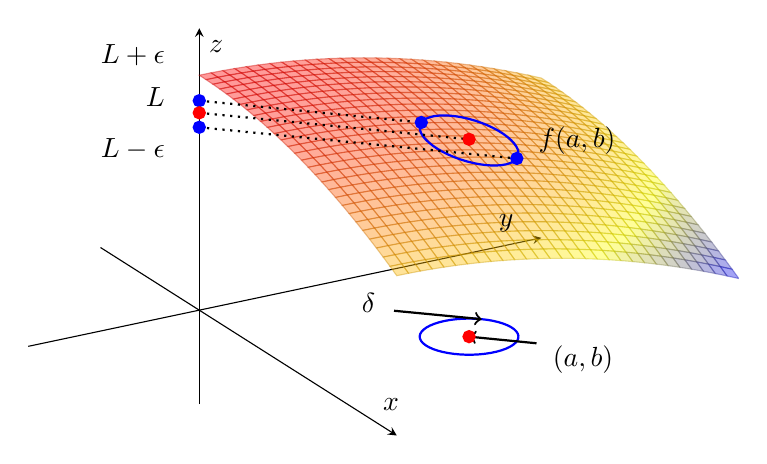
\begin{tikzpicture}
  \begin{axis}[
      view={60}{30}, % Adjust the viewing angle
      xlabel={$x$}, ylabel={$y$}, zlabel={$z$},
      axis lines=middle,
      xmin=-2, xmax=4,
      ymin=-2, ymax=4,
      zmin=-2, zmax=6,
      grid=major,
      ticks=none,
      scale=1.5, % Scales the geometries (axes, lines, surfaces)
      label style={font=\normalsize}, % Keeps label sizes the same
      tick label style={font=\small}, % Keeps tick labels consistent
  ]
      % Delta circle in the x-y plane
      \addplot3[samples=50,domain=0:360,thick,blue]
        ({2 - 0.5*cos(x)},{2 - 0.5*sin(x)},{0});
      
      % Dot at (a, b) in the x-y plane
      \addplot3[only marks, mark=*, mark options={red}, thick] coordinates {(2,2,0)};
      
      % Callout to (a, b)
      \draw[->,thick] (axis cs:2.5,2.5,0) -- (axis cs:2,2,0);
      \node[above right] at (axis cs:3.5,2,0) {$(a, b)$};
      
      % Callout to delta (radius size)
      \draw[->,thick] (axis cs:1,1.7,0) -- (axis cs:1.646,2.353,0);
      \node[below left] at (axis cs:0.3,2,0) {$\delta$};
      
      % Transparent surface above the x-y plane
      \addplot3[surf,opacity=0.4,samples=30,samples y=30,domain=0:4,y domain=0:4]
        {5 - 0.1*(x^2 + y^2)};
      
      % Dot at (a, b) on the surface
      \addplot3[only marks, mark=*, mark options={red}, thick] coordinates {(2,2,{5 - 0.1*(2^2 + 2^2)})};
      
      % Movable label for f(a,b)
      \node at (axis cs:2.8,2.8,{5 - 0.1*(2^2 + 2^2) + 0.2}) {$f(a,b)$};
      
      % Circle on the surface
      \addplot3[samples=50,domain=0:360,thick,blue]
        ({2 - 0.5*cos(x)},{2 - 0.5*sin(x)},{5 - 0.1*((2 - 0.5*cos(x))^2 + (2 - 0.5*sin(x))^2)});
      
      % Maximum height point on the circle on the surface
      \addplot3[only marks, mark=*, mark options={blue}, thick] 
        coordinates {(1.646, 1.646, 4.458)};
      
      % Minimum height point on the circle on the surface
      \addplot3[only marks, mark=*, mark options={blue}, thick] 
        coordinates {(2.354, 2.354, 3.892)};
      
      % Blue dot for L + epsilon on z-axis
      \addplot3[only marks, mark=*, mark options={blue}, thick] coordinates {(0, 0, 4.458)};
      \node[left] at (axis cs:-0.5, 0, 5.1) {$L + \epsilon$};

      % Blue dot for L - epsilon on z-axis
      \addplot3[only marks, mark=*, mark options={blue}, thick] coordinates {(0, 0, 3.892)};
      \node[left] at (axis cs:-0.5, 0, 3.1) {$L - \epsilon$};
      
      % Red dot for L on z-axis
      \addplot3[only marks, mark=*, mark options={red}, thick] coordinates {(0, 0, {5 - 0.1*(2^2 + 2^2)})};
      \node[left] at (axis cs:-0.5, 0, {5 - 0.1*(2^2 + 2^2)}) {$L$};
      
      % Dotted line from L + epsilon to maximum height on the surface
      \draw[dotted, thick] (axis cs:0,0,4.458) -- (axis cs:1.646,1.646,4.458);
      
      % Dotted line from L to f(a,b) on the surface
      \draw[dotted, thick] (axis cs:0,0,{5 - 0.1*(2^2 + 2^2)}) -- (axis cs:2,2,{5 - 0.1*(2^2 + 2^2)});
      
      % Dotted line from L - epsilon to minimum height on the surface
      \draw[dotted, thick] (axis cs:0,0,3.892) -- (axis cs:2.354,2.354,3.892);
  \end{axis}
\end{tikzpicture}
    \caption{\textit{Visualization of the \(\varepsilon\)-\(\delta\) definition for a function of two variables. The blue circle of radius \(\delta\) in the \(xy\)-plane surrounds \((a,b)\). The surface \(z = f(x,y)\) is shown with the corresponding curve on the surface above the \(\delta\)-circle. The values \(L + \varepsilon\) and \(L - \varepsilon\) on the \(z\)-axis mark the acceptable output range: the definition requires that whenever \((x,y)\) lies within the \(\delta\)-circle, the surface height stays between \(L - \varepsilon\) and \(L + \varepsilon\).}}
\end{figure}



\noindent The concept of limits extends to functions of three or more variables. For a function \( f(x, y, z) \), the limit as \( (x, y, z) \to (a, b, c) \) is defined similarly:
\[
\lim_{(x, y, z) \to (a, b, c)} f(x, y, z) = L
\]
if for every \( \epsilon > 0 \), there exists a \( \delta > 0 \) such that:
\[
0 < \sqrt{(x-a)^2 + (y-b)^2 + (z-c)^2} < \delta \implies |f(x, y, z) - L| < \epsilon.
\]
The principles remain the same, but the added dimension increases the complexity of path dependence and visualization. Tools like polar, cylindrical, or spherical coordinates are often used to simplify calculations. \\

\noindent This idea generalizes further to functions of \( n \)-variables, \( f(x_1, x_2, \dots, x_n) \). The limit as \( (x_1, x_2, \dots, x_n) \to (a_1, a_2, \dots, a_n) \) is defined as:
\[
\lim_{(x_1, x_2, \dots, x_n) \to (a_1, a_2, \dots, a_n)} f(x_1, x_2, \dots, x_n) = L
\]
if for every \( \epsilon > 0 \), there exists a \( \delta > 0 \) such that:
\[
0 < \sqrt{\sum_{i=1}^n (x_i - a_i)^2} < \delta \implies |f(x_1, x_2, \dots, x_n) - L| < \epsilon.
\]
Here, the distance metric generalizes to the Euclidean norm in \( n \)-dimensional space:
\[
\sqrt{\sum_{i=1}^n (x_i - a_i)^2},
\]
which measures the distance between the point \( (x_1, x_2, \dots, x_n) \) and the target \( (a_1, a_2, \dots, a_n) \). The \(\epsilon\)-\(\delta\) framework ensures that as \( (x_1, x_2, \dots, x_n) \) approaches \( (a_1, a_2, \dots, a_n) \) in this generalized space, the function value \( f(x_1, x_2, \dots, x_n) \) approaches \( L \), independent of the path taken. \\
\noindent Alternatively, the concept of limits can be compactly expressed using vector notation. For a function \( f(\mathbf{x}) \) where \( \mathbf{x} = (x_1, x_2, \dots, x_n) \) and the target point is \( \mathbf{a} = (a_1, a_2, \dots, a_n) \), the limit is written as:
\[
\lim_{\mathbf{x} \to \mathbf{a}} f(\mathbf{x}) = L,
\]
if for every \( \epsilon > 0 \), there exists a \( \delta > 0 \) such that:
\[
0 < \|\mathbf{x} - \mathbf{a}\| < \delta \implies |f(\mathbf{x}) - L| < \epsilon.
\]

\exampleline
\begin{example}
Using the formal definition of limits for multivariable functions, prove that:
\[
\lim_{(x, y) \to (0, 0)} x y = 0.
\]


\begin{solution}
To prove that:
\[
\lim_{(x, y) \to (0, 0)} x y = 0,
\]
we need to show that for every \( \epsilon > 0 \), there exists a \( \delta > 0 \) such that whenever \( 0 < \sqrt{(x - 0)^2 + (y - 0)^2} < \delta \), it follows that:
\[
|x y - 0| < \epsilon.
\]

\noindent \textbf{Proof:} Let \( \epsilon > 0 \) be given. We aim to find \( \delta > 0 \) such that if \( 0 < \sqrt{x^2 + y^2} < \delta \), then \( |x y| < \epsilon \). Note that since \( |x| \leq \sqrt{x^2 + y^2} \) and \( |y| \leq \sqrt{x^2 + y^2} \), we have:
\[
|x y| = |x||y| \leq \left( \sqrt{x^2 + y^2} \right) \left( \sqrt{x^2 + y^2} \right) = \left( \sqrt{x^2 + y^2} \right)^2.
\]

\noindent Now, choose \( \delta = \sqrt{\epsilon} \). Then \( \delta > 0 \) because \( \epsilon > 0 \). Suppose \( 0 < \sqrt{x^2 + y^2} < \delta \). Then:
\[
|x y| \leq \left( \sqrt{x^2 + y^2} \right)^2 < \delta^2 = (\sqrt{\epsilon})^2 = \epsilon.
\]

\noindent  Therefore, whenever \( 0 < \sqrt{x^2 + y^2} < \delta \), it follows that \( |x y| < \epsilon \). \\

\noindent  \textbf{Conclusion:} For every \( \epsilon > 0 \), we have found \( \delta = \sqrt{\epsilon} > 0 \) such that:
\[
0 < \sqrt{x^2 + y^2} < \delta \implies |x y - 0| < \epsilon.
\]
\noindent  Hence, by the formal definition of limits for multivariable functions,
\[
\lim_{(x, y) \to (0, 0)} x y = 0.
\]
\end{solution}
\end{example}
\exampleline


\subsection*{Continuity in Multivariable Functions} \index{Continuous Functions}

\noindent Continuity is a fundamental concept in calculus, naturally extending from single-variable functions to multivariable functions. Intuitively, a function \( f(x, y) \) is continuous at a point \( (a, b) \) if small changes in \( (x, y) \) near \( (a, b) \) result in small changes in \( f(x, y) \). Formally, \( f(x, y) \) is continuous at \( (a, b) \) if:
\[
\lim_{(x, y) \to (a, b)} f(x, y) = f(a, b).
\]
This definition implies three necessary conditions:
\begin{enumerate}
    \item \( f(x, y) \) is defined at \( (a, b) \).
    \item The limit \( \lim_{(x, y) \to (a, b)} f(x, y) \) exists.
    \item The limit equals the function value: \( \lim_{(x, y) \to (a, b)} f(x, y) = f(a, b) \).
\end{enumerate}
The idea of continuity in multiple dimensions generalizes the familiar notion of a smooth, unbroken curve or surface.

\paragraph{Visualizing Continuity:}
To better understand continuity, imagine a surface in three-dimensional space representing \( z = f(x, y) \). Continuity at a point \( (a, b) \) ensures that as \( (x, y) \) approaches \( (a, b) \) from any direction, the surface height \( z \) converges to a single value \( f(a, b) \). Discontinuities manifest as abrupt breaks, gaps, or sharp jumps in the surface, where the smoothness of the surface is compromised. A simple example of a continuous function is \( f(x, y) = x^2 + y^2 \), which forms a paraboloid, while a function like \( f(x, y) = \frac{1}{x^2 + y^2} \) is discontinuous at \( (0, 0) \), as the value of \( f(x, y) \) becomes unbounded near this point.

\paragraph{Continuity on a Domain:}
A function \( f(x, y) \) is continuous on a region \( R \subseteq \mathbb{R}^2 \) if it is continuous at every point \( (x, y) \in R \). These regions can be:
\begin{itemize}
    \item \textbf{Open Regions:} Regions excluding their boundary points, such as the interior of a circle.
    \item \textbf{Closed Regions:} Regions including their boundary points, such as a closed square or disk.
    \item \textbf{Bounded and Unbounded Regions:} Continuity can be considered within finite or infinite domains.
\end{itemize}
For example, the function \( f(x, y) = x^2 + y^2 \) is continuous everywhere on \( \mathbb{R}^2 \), while \( f(x, y) = \frac{1}{x^2 + y^2} \) is continuous only on \( \mathbb{R}^2 \setminus \{(0, 0)\} \).

\paragraph{Properties of Continuous Functions:}
Multivariable functions share several properties of continuous single-variable functions, providing tools for analyzing their behavior:
\begin{itemize}
    \item \textbf{Sum, Difference, and Product:} If \( f \) and \( g \) are continuous at \( (a, b) \), then \( f+g \), \( f-g \), and \( fg \) are also continuous at \( (a, b) \).
    \item \textbf{Quotients:} If \( f \) and \( g \) are continuous at \( (a, b) \) and \( g(a, b) \neq 0 \), then \( f/g \) is continuous at \( (a, b) \).
    \item \textbf{Composition:} If \( f \) is continuous at \( (a, b) \) and \( g \) is continuous at \( f(a, b) \), then \( g \circ f \) is continuous at \( (a, b) \).
\end{itemize}

\paragraph{Discontinuities:}
Discontinuities in multivariable functions can be classified as:
\begin{itemize}
    \item \textbf{Removable Discontinuities:} Occur when a limit exists at \( (a, b) \) but does not equal \( f(a, b) \). For example, a ``hole" in the surface can be filled by redefining \( f(a, b) \) to match the limit.
    \item \textbf{Jump Discontinuities:} Occur when the limit does not exist due to different values along different paths. For instance, consider \( f(x, y) = \begin{cases} 
    1 & \text{if } x = 0, \\
    0 & \text{if } x \neq 0.
    \end{cases} \)
    \item \textbf{Essential Discontinuities:} Occur when no limit exists at \( (a, b) \), such as in functions with oscillatory behavior near \( (a, b) \).
\end{itemize}

\paragraph{High-Dimensional Analogues of Theorems:} \index{Intermediate Value Theorem}
Several familiar theorems from single-variable calculus extend to multivariable functions, often requiring additional assumptions or interpretations. Note that some terminology and notation will be further revealed in later chapters as they become relevant.

\begin{itemize} \index{Intermediate Value Theorem}
    \item \textbf{Intermediate Value Theorem:} If \( f(x, y) \) is continuous on a connected region \( R \) and takes on two distinct values \( a \) and \( b \), then \( f(x, y) \) takes every value between \( a \) and \( b \) at some point in \( R \). This is particularly useful in multivariable optimization problems or proving the existence of level curves.
    
    \item \textbf{Mean Value Theorem:} \index{Mean Value Theorem} A multivariable generalization of the MVT states that for a differentiable function \( f \) and points \( \mathbf{a}, \mathbf{b} \) in a convex domain, there exists a point \( \mathbf{c} \) on the line segment from \( \mathbf{a} \) to \( \mathbf{b} \) such that \( f(\mathbf{b}) - f(\mathbf{a}) = \nabla f(\mathbf{c}) \cdot (\mathbf{b} - \mathbf{a}) \).

    \item \textbf{Extreme Value Theorem:} \index{Extreme Value Theorem} If \( f(x, y, z) \) is continuous on a closed and bounded region \( R \subseteq \mathbb{R}^3 \), then \( f \) attains both a maximum and minimum value on \( R \). This theorem underpins much of multivariable optimization, particularly when combined with Lagrange multipliers.

    \item \textbf{Squeeze Theorem:} \index{Squeeze Theorem} The multivariable version states that if \( g(x, y) \leq f(x, y) \leq h(x, y) \) for all \( (x, y) \in R \), and \( \lim_{(x, y) \to (a, b)} g(x, y) = \lim_{(x, y) \to (a, b)} h(x, y) = L \), then \( \lim_{(x, y) \to (a, b)} f(x, y) = L \). This theorem is invaluable in proving the existence of limits.

\end{itemize}

\exampleline
\begin{example}
Verify the Intermediate Value Theorem for the function 
\[
f(x, y) = x^2 + y^2 - 1
\]
on the closed region \( R = \{(x, y) \in \mathbb{R}^2 \mid -1 \leq x, y \leq 1\} \), and show that there exists a point \( (a, b) \in R \) such that \( f(a, b) = 0 \).

\begin{solution}
The function \( f(x, y) = x^2 + y^2 - 1 \) is a polynomial in \( x \) and \( y \), so it is continuous on \( \mathbb{R}^2 \), including the closed and bounded region \( R \). 

\begin{itemize}
    \item \textbf{Step 1: Evaluate \( f \) at specific points in \( R \).}
    At \( (-1, 0) \), we have:
    \[
    f(-1, 0) = (-1)^2 + 0^2 - 1 = 0.
    \]
    At \( (0, 0) \), we have:
    \[
    f(0, 0) = 0^2 + 0^2 - 1 = -1.
    \]
    At \( (1, 1) \), we have:
    \[
    f(1, 1) = 1^2 + 1^2 - 1 = 1.
    \]

    \item \textbf{Step 2: Apply the Intermediate Value Theorem.}
    Because \( f(x, y) \) is continuous on \( R \), and \( f(-1, 0) = 0 \), \( f(0, 0) = -1 \), and \( f(1, 1) = 1 \), it must take every value between \( -1 \) and \( 1 \) at some point in \( R \). 

    In particular, since \( f(-1, 0) = 0 \), there is no further verification needed to show that \( f(x, y) = 0 \) holds within \( R \). However, the Intermediate Value Theorem guarantees that \( f(x, y) = c \) for any \( c \in [-1, 1] \).

    \item \textbf{Conclusion:} The Intermediate Value Theorem verifies that there exists a point \( (a, b) \in R \), such as \( (-1, 0) \), where \( f(a, b) = 0 \).
\end{itemize}
\end{solution}
\end{example}
\exampleline


\newpage











\lecture{Partial Derivatives} \index{Partial Derivatives}

\noindent Imagine you’re at an all-you-can-eat buffet. You’ve loaded your plate with chicken, mashed potatoes, and gravy, but now you’re debating how many meatballs to pile on. The chicken is staying put, the mashed potatoes aren’t going anywhere, and the gravy is committed to the cause—but the meatballs? They’re the variable. This is partial derivatives in a nutshell: you’re holding everything else constant while analyzing how one particular choice impacts your meal (or, in this case, your mathematical function). Just as you ask, ``How many meatballs is too many?" partial derivatives ask, ``How does the function change if only one variable changes?" This section explores the formal definition, interpretation, and properties of partial derivatives, including higher-order derivatives and Clairaut's theorem.

\subsection*{Definition and Notation}

\noindent Recall from single-variable calculus that the derivative of a function \( f(x) \) at a point \( x = a \) is defined as:
\[
f'(a) = \lim_{h \to 0} \frac{f(a + h) - f(a)}{h},
\]
which measures the instantaneous rate of change of \( f(x) \) with respect to \( x \). This idea naturally extends to functions of several variables by allowing one variable to change while holding others constant. For a function \( f(x, y) \) defined in a region of \( \mathbb{R}^2 \), we define the \textit{partial derivative} of \( f \) with respect to \( x \), denoted \( \frac{\partial f}{\partial x} \) or \( f_x \), as:
\[
\frac{\partial f}{\partial x}(x, y) = \lim_{h \to 0} \frac{f(x + h, y) - f(x, y)}{h},
\]
provided the limit exists. Here, \( y \) is held constant, and \( x \) is allowed to vary. Similarly, the partial derivative with respect to \( y \) is defined as:
\[
\frac{\partial f}{\partial y}(x, y) = \lim_{h \to 0} \frac{f(x, y + h) - f(x, y)}{h}.
\]

\noindent This definition can be understood as a direct application of the single-variable derivative, applied to one variable at a time. By holding one variable fixed, we reduce the function \( f(x, y) \) to a single-variable function, enabling us to compute its rate of change with respect to the variable of interest. \\

\noindent For functions of three or more variables, such as \( f(x_1, x_2, \ldots, x_n) \), the partial derivative with respect to \( x_i \) is similarly defined:
\[
\frac{\partial f}{\partial x_i}(x_1, x_2, \ldots, x_n) = \lim_{h \to 0} \frac{f(x_1, \ldots, x_i + h, \ldots, x_n) - f(x_1, \ldots, x_i, \ldots, x_n)}{h},
\]
where only \( x_i \) is perturbed, while all other variables are held constant. This generalization allows us to study functions in higher-dimensional spaces, providing a foundation for advanced topics like gradients and optimization. 


\exampleline
\begin{example}
Use the limit definition of a partial derivative to compute \( \frac{\partial f}{\partial x} \) for \( f(x, y) = x^2y + 3xy^2 \).

\begin{solution}
\noindent Recall the limit definition of the partial derivative:
\[
\frac{\partial f}{\partial x}(x, y) = \lim_{h \to 0} \frac{f(x + h, y) - f(x, y)}{h}.
\]
Substitute \( f(x, y) = x^2y + 3xy^2 \) into the definition:
\[
\frac{\partial f}{\partial x}(x, y) = \lim_{h \to 0} \frac{f(x + h, y) - f(x, y)}{h}.
\]
Compute \( f(x + h, y) \):
\[
f(x + h, y) = (x + h)^2y + 3(x + h)y^2.
\]
Expand the terms:
\[
f(x + h, y) = (x^2 + 2xh + h^2)y + 3(xy^2 + hy^2) = x^2y + 2xhy + h^2y + 3xy^2 + 3hy^2.
\]
Now subtract \( f(x, y) \):
\[
f(x + h, y) - f(x, y) = (x^2y + 2xhy + h^2y + 3xy^2 + 3hy^2) - (x^2y + 3xy^2).
\]
Simplify:
\[
f(x + h, y) - f(x, y) = 2xhy + h^2y + 3hy^2.
\]
Divide by \( h \):
\[
\frac{f(x + h, y) - f(x, y)}{h} = \frac{2xhy + h^2y + 3hy^2}{h}.
\]
Simplify further:
\[
\frac{f(x + h, y) - f(x, y)}{h} = 2xy + hy + 3y^2.
\]
Take the limit as \( h \to 0 \):
\[
\lim_{h \to 0} \frac{f(x + h, y) - f(x, y)}{h} = 2xy + 3y^2.
\]
Thus:
\[
\frac{\partial f}{\partial x}(x, y) = 2xy + 3y^2.
\]
\end{solution}
\end{example}
\exampleline


\noindent The partial derivative \( \frac{\partial f}{\partial x}(x, y) \) measures the rate of change of \( f(x, y) \) with respect to \( x \), while keeping \( y \) fixed. Geometrically, this corresponds to the slope of the tangent line to the curve obtained by intersecting the surface \( z = f(x, y) \) with the plane \( y = \text{constant} \). Similarly, \( \frac{\partial f}{\partial y} \) represents the slope of the tangent line to the curve obtained by intersecting the surface with the plane \( x = \text{constant} \). These partial derivatives capture the local behavior of the surface along the coordinate axes. \\

\noindent Several standard notations are used for partial derivatives, depending on the context:
\begin{itemize}
    \item \( \frac{\partial f}{\partial x} \): Highlights the operator \( \partial \), distinguishing it from total derivatives.
    \item \( f_x \): A compact notation often used in applied contexts.
    \item \( \partial_x f \): A concise form useful in symbolic computation and advanced texts.
\end{itemize}

\noindent These notations emphasize that partial derivatives focus on the effect of one variable at a time, isolating its contribution to the overall behavior of \( f(x, y) \). By leveraging the limit definition and geometric intuition, we gain a comprehensive understanding of how multivariable functions behave locally in their domains.


\begin{figure}[H]
    \centering
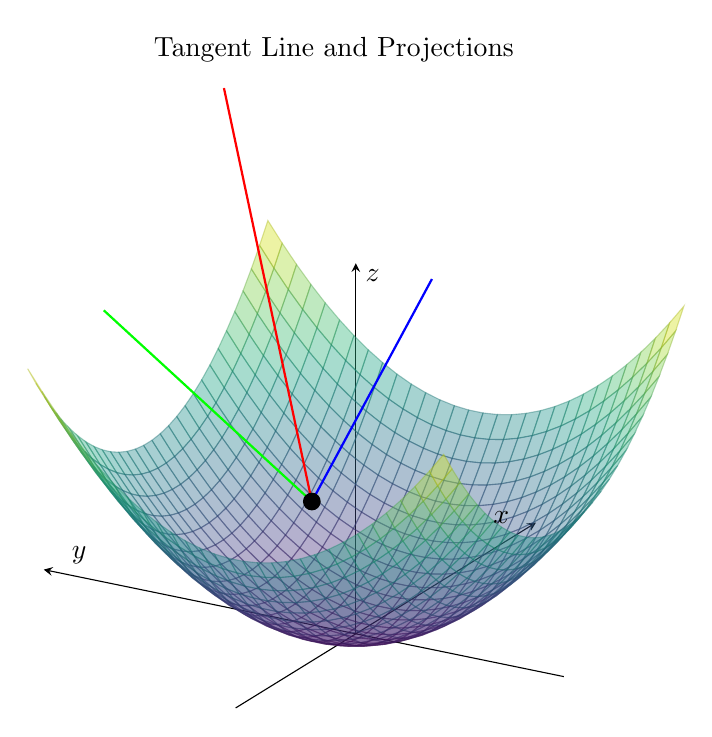
\begin{tikzpicture}
  \begin{axis}[
      view={-60}{30},
      axis lines=center,
      xlabel={$x$},
      ylabel={$y$},
      zlabel={$z$},
      width=12cm,
      height=10cm,
      ticks=none,
      title={Tangent Line and Projections}
    ]

    % Plot the surface z = x^2 + y^2
    \addplot3[
      surf,
      opacity=0.4,
      samples=30,
      samples y=30,
      domain=-2:2,
      y domain=-2:2,
      colormap/viridis
    ]
    {x^2 + y^2};

    % Tangent line at point (1, 1, 2)
    % Equation: z = 2 + 2(x - 1) + 2(y - 1)
    \addplot3[
      thick,
      color=red,
      domain=0:2
    ]
    (1 + x, 1 + x, {2 + 2*x + 2*x});

    % Projection of tangent line onto the xz-plane (y = constant)
    \addplot3[
      thick,
      dashed,
      color=blue,
      domain=0:2
    ]
    (1 + x, 1, {2 + 2*x});

    % Projection of tangent line onto the yz-plane (x = constant)
    \addplot3[
      thick,
      dashed,
      color=green,
      domain=0:2
    ]
    (1, 1 + x, {2 + 2*x});

    % Mark the point of tangency
    \addplot3[
      only marks,
      mark=*,
      mark size=3pt,
      color=black
    ]
    coordinates {(1, 1, 2)};
   


  \end{axis}
\end{tikzpicture}
 \caption{\textit{Derivative of a surface $z = x^2 + y^2$ at a point $(1,1,2)$. The tangent line (red) is notated with projections of each component, green indicating $yz$-plane projection of the tangent line, and blue indicating the $xz$-plane projection.}}
 \label{fig:derivative_high_order}
\end{figure}


\subsubsection*{Basic Properties of Partial Derivatives.}
Partial derivatives share many properties with single-variable derivatives. The following are some fundamental properties of partial derivatives that are useful for computation and analysis:

\begin{itemize}
    \item \textbf{Linearity:} If \( f(x, y) \) and \( g(x, y) \) are differentiable functions, and \( c \) is a constant, then:
    \[
    \frac{\partial}{\partial x}(cf(x, y) + g(x, y)) = c\frac{\partial f}{\partial x} + \frac{\partial g}{\partial x}.
    \]

    \item \textbf{Product Rule:} If \( f(x, y) \) and \( g(x, y) \) are differentiable, then:
    \[
    \frac{\partial}{\partial x}(f(x, y)g(x, y)) = f_x g + f g_x.
    \]

    \item \textbf{Quotient Rule:} If \( f(x, y) \) and \( g(x, y) \) are differentiable, and \( g(x, y) \neq 0 \), then:
    \[
    \frac{\partial}{\partial x}\left(\frac{f(x, y)}{g(x, y)}\right) = \frac{f_x g - f g_x}{g^2}.
    \]

    \item \textbf{Chain Rule (Simple Form):} If \( z = f(x, y) \), where \( x \) and \( y \) are functions of another variable \( t \), then:
    \[
    \frac{dz}{dt} = \frac{\partial f}{\partial x} \frac{dx}{dt} + \frac{\partial f}{\partial y} \frac{dy}{dt}.
    \]
	The chain rule gets a little hairy, and hence we will dedicate an entire lecture to it later on.
    \item \textbf{Zero Partial Derivative:} If \( \frac{\partial f}{\partial x} = 0 \) in a region, then \( f(x, y) \) does not change with \( x \) in that region (it depends only on \( y \)).

    \item \textbf{Partial Derivatives of Constants:} If \( c \) is a constant, then:
    \[
    \frac{\partial c}{\partial x} = 0 \quad \text{and} \quad \frac{\partial c}{\partial y} = 0.
    \]
\end{itemize}


\exampleline
\begin{example}
Compute the partial derivatives of the following functions with respect to all specified variables:
\begin{enumerate}
    \item \( f(x, y) = x^2y + 3xy^2 \) (with respect to \( x \) and \( y \))
    \item \( g(x, y, z) = e^{xz} \sin(y) \) (with respect to \( x \), \( y \), and \( z \))
    \item \( h(x, y) = \frac{x^2 + y^2}{x - y} \) (with respect to \( x \) and \( y \))
\end{enumerate}

\begin{solution}
\begin{enumerate}
    \item For \( f(x, y) = x^2y + 3xy^2 \):
    \begin{itemize}
        \item Partial derivative with respect to \( x \):
        \[
        \frac{\partial f}{\partial x} = \frac{\partial}{\partial x}(x^2y) + \frac{\partial}{\partial x}(3xy^2) = 2xy + 3y^2.
        \]
        \item Partial derivative with respect to \( y \):
        \[
        \frac{\partial f}{\partial y} = \frac{\partial}{\partial y}(x^2y) + \frac{\partial}{\partial y}(3xy^2) = x^2 + 6xy.
        \]
    \end{itemize}

    \item For \( g(x, y, z) = e^{xz} \sin(y) \):
    \begin{itemize}
        \item Partial derivative with respect to \( x \):
        \[
        \frac{\partial g}{\partial x} = \frac{\partial}{\partial x}\left(e^{xz} \sin(y)\right) = z e^{xz} \sin(y).
        \]
        \item Partial derivative with respect to \( y \):
        \[
        \frac{\partial g}{\partial y} = \frac{\partial}{\partial y}\left(e^{xz} \sin(y)\right) = e^{xz} \cos(y).
        \]
        \item Partial derivative with respect to \( z \):
        \[
        \frac{\partial g}{\partial z} = \frac{\partial}{\partial z}\left(e^{xz} \sin(y)\right) = x e^{xz} \sin(y).
        \]
    \end{itemize}

    \item For \( h(x, y) = \frac{x^2 + y^2}{x - y} \):
    \begin{itemize}
        \item Partial derivative with respect to \( x \) (using the quotient rule):
        \[
        \frac{\partial h}{\partial x} = \frac{(2x)(x - y) - (x^2 + y^2)(1)}{(x - y)^2} = \frac{2x(x - y) - (x^2 + y^2)}{(x - y)^2}.
        \]
        Simplify:
        \[
        \frac{\partial h}{\partial x} = \frac{x^2 - 2xy - y^2}{(x - y)^2}.
        \]
        \item Partial derivative with respect to \( y \) (using the quotient rule):
        \[
        \frac{\partial h}{\partial y} = \frac{(2y)(x - y) - (x^2 + y^2)(-1)}{(x - y)^2} = \frac{2y(x - y) + (x^2 + y^2)}{(x - y)^2}.
        \]
        Simplify:
        \[
        \frac{\partial h}{\partial y} = \frac{x^2 + 2xy - y^2}{(x - y)^2}.
        \]
    \end{itemize}
\end{enumerate}
\end{solution}
\end{example}
\exampleline

\subsection*{Higher-Order Partial Derivatives} \index{Higher-Order Partial Derivatives}

\noindent Higher-order partial derivatives extend the concept of derivatives to capture rates of change of rates of change, just as in single-variable calculus. For a function \( f(x, y) \), the second-order partial derivatives include:
\[
\frac{\partial^2 f}{\partial x^2}, \quad \frac{\partial^2 f}{\partial y^2}, \quad \text{and} \quad \frac{\partial^2 f}{\partial x \partial y}, \quad \frac{\partial^2 f}{\partial y \partial x}.
\]

\noindent These derivatives are often written more compactly using subscript notation:
\[
f_{xx} = \frac{\partial^2 f}{\partial x^2}, \quad f_{yy} = \frac{\partial^2 f}{\partial y^2}, \quad f_{xy} = \frac{\partial^2 f}{\partial x \partial y}, \quad f_{yx} = \frac{\partial^2 f}{\partial y \partial x}.
\]

\noindent These derivatives reveal local properties of the function, such as curvature, along specific directions. Mixed partial derivatives, such as \( \frac{\partial^2 f}{\partial x \partial y} \) or \( f_{xy} \), involve differentiating first with respect to one variable and then with respect to another:
\[
\frac{\partial^2 f}{\partial x \partial y} = \frac{\partial}{\partial y} \left( \frac{\partial f}{\partial x} \right), \quad \text{or equivalently,} \quad f_{xy} = \frac{\partial}{\partial y} \left( f_x \right),
\]
\[
\frac{\partial^2 f}{\partial y \partial x} = \frac{\partial}{\partial x} \left( \frac{\partial f}{\partial y} \right), \quad \text{or equivalently,} \quad f_{yx} = \frac{\partial}{\partial x} \left( f_y \right).
\]

\noindent Note: we adopt the convention that \( f_{xy} \) means first differentiate with respect to \( x \), then with respect to \( y \). Some references use the opposite convention; when in doubt, the subscript order \( f_{xy} = (f_x)_y \) is unambiguous.

\noindent This naturally extends to higher dimensions. For a function \( f(x_1, x_2, \ldots, x_n) \), higher-order derivatives can be computed repeatedly by differentiating with respect to different variables. For example, the general \( k \)-th order partial derivative is denoted as:
\[
\frac{\partial^k f}{\partial x_{i_1} \partial x_{i_2} \cdots \partial x_{i_k}},
\]
where \( i_1, i_2, \ldots, i_k \) indicate the sequence of variables being differentiated. Using subscript notation, this becomes:
\[
f_{x_{i_1}x_{i_2}\cdots x_{i_k}},
\]
highlighting the order of differentiation. This generalization mirrors the iterative process of differentiation from single-variable calculus. \\

\noindent These derivatives are vital in analyzing the behavior of multivariable functions. For instance:
\begin{itemize}
    \item \textbf{Curvature Analysis:} Second-order derivatives reveal concavity and convexity, analogous to the second derivative test in single-variable calculus.
    \item \textbf{Critical Points:} Higher-order partial derivatives help identify extrema and saddle points, topics that will be discussed in a future lecture.
    \item \textbf{Taylor Expansions:} Higher-order derivatives are fundamental in approximating functions using Taylor series in multiple dimensions.
\end{itemize}

\paragraph{Does the Order of Differentiation Matter?}
A natural question arises: does the order of differentiation affect the result? That is, is:
\[
\frac{\partial^2 f}{\partial x \partial y} \stackrel{?}{=} \frac{\partial^2 f}{\partial y \partial x}?
\]

\noindent Surprisingly—or perhaps reassuringly—the answer is that the order generally does \textit{not} matter, provided certain conditions are met. 


\subsection*{Clairaut's Theorem on Mixed Partial Derivatives} \index{Clairaut's Theorem}

\noindent Clairaut's Theorem states that if \( f \) is defined on a region \( R \subseteq \mathbb{R}^n \) and all second-order partial derivatives of \( f \) are continuous on \( R \), then the mixed partial derivatives are equal:
\[
\frac{\partial^2 f}{\partial x \partial y} = \frac{\partial^2 f}{\partial y \partial x}.
\]

\noindent This result is both powerful and intuitive, as it guarantees symmetry in the order of differentiation under appropriate continuity conditions. To generalize, for \( f(x_1, x_2, \ldots, x_n) \):
\[
\frac{\partial^2 f}{\partial x_i \partial x_j} = \frac{\partial^2 f}{\partial x_j \partial x_i}, \quad \text{for all } i, j \text{ such that the derivatives are continuous.}
\]

\paragraph{Proof Outline of Clairaut's Theorem.}
The proof relies on the definition of partial derivatives and the interchangeability of limits for continuous functions:
\begin{enumerate}
    \item Write the mixed partial derivative \( \frac{\partial^2 f}{\partial x \partial y} \) as:
    \[
    \frac{\partial^2 f}{\partial x \partial y} = \lim_{h \to 0} \frac{\frac{\partial f}{\partial x}(x, y + h) - \frac{\partial f}{\partial x}(x, y)}{h}.
    \]
    \item Substitute the definition of \( \frac{\partial f}{\partial x} \) in terms of limits, and observe that the nested limits commute if \( f \) is continuous.
    \item Symmetry emerges from the commutativity of the limits, leading to:
    \[
    \frac{\partial^2 f}{\partial x \partial y} = \frac{\partial^2 f}{\partial y \partial x}.
    \]
    \item Continuity of the second-order partial derivatives ensures the validity of this reasoning.
\end{enumerate}

\paragraph{Counterexample:}
Consider the function \( f(x, y) \) defined as:
\[
f(x, y) = 
\begin{cases} 
\frac{xy(x^2 - y^2)}{x^2 + y^2}, & \text{if } (x, y) \neq (0, 0), \\
0, & \text{if } (x, y) = (0, 0).
\end{cases}
\]

\noindent Compute the mixed partial derivatives at \( (0, 0) \) using the limit definition. First, one can show that:
\[
f_x(0, y) = -y, \qquad f_y(x, 0) = x.
\]
Then:
\[
f_{xy}(0,0) = \lim_{h \to 0} \frac{f_x(0, h) - f_x(0, 0)}{h} = \lim_{h \to 0} \frac{-h - 0}{h} = -1,
\]
\[
f_{yx}(0,0) = \lim_{h \to 0} \frac{f_y(h, 0) - f_y(0, 0)}{h} = \lim_{h \to 0} \frac{h - 0}{h} = 1.
\]
Since \( f_{xy}(0,0) = -1 \neq 1 = f_{yx}(0,0) \), the mixed partial derivatives are not equal.

\noindent This failure arises because the second-order partial derivatives of \( f \) are not continuous at \( (0, 0) \), violating the conditions of Clairaut's Theorem. \\

\noindent Note: the existence of partial derivatives does not guarantee the continuity of a function. A function can have partial derivatives at a point without being continuous there. However, if all partial derivatives are continuous in a region, the function is said to be \textit{continuously differentiable}, denoted \( C^1 \). This property is critical for advanced topics, such as optimization and differential equations.

\exampleline
\begin{example}
Verify Clairaut's Theorem for the following functions:
\begin{enumerate}
    \item \( f(x, y) = x^2y + y^3 \)
    \item \( f(x, y) = e^{xy} \)
\end{enumerate}

\begin{solution}
\begin{enumerate}
    \item For \( f(x, y) = x^2y + y^3 \):
    \begin{itemize}
        \item Compute \( \frac{\partial f}{\partial x} \):
        \[
        \frac{\partial f}{\partial x} = \frac{\partial}{\partial x} (x^2y + y^3) = 2xy.
        \]
        \item Compute \( \frac{\partial^2 f}{\partial x \partial y} \):
        \[
        \frac{\partial^2 f}{\partial x \partial y} = \frac{\partial}{\partial y} (2xy) = 2x.
        \]
        \item Compute \( \frac{\partial f}{\partial y} \):
        \[
        \frac{\partial f}{\partial y} = \frac{\partial}{\partial y} (x^2y + y^3) = x^2 + 3y^2.
        \]
        \item Compute \( \frac{\partial^2 f}{\partial y \partial x} \):
        \[
        \frac{\partial^2 f}{\partial y \partial x} = \frac{\partial}{\partial x} (x^2 + 3y^2) = 2x.
        \]
        Since \( \frac{\partial^2 f}{\partial x \partial y} = \frac{\partial^2 f}{\partial y \partial x} = 2x \), Clairaut's Theorem is verified.

    \end{itemize}

    \item For \( f(x, y) = e^{xy} \):
    \begin{itemize}
        \item Compute \( \frac{\partial f}{\partial x} \):
        \[
        \frac{\partial f}{\partial x} = \frac{\partial}{\partial x} (e^{xy}) = ye^{xy}.
        \]
        \item Compute \( \frac{\partial^2 f}{\partial x \partial y} \):
        \[
        \frac{\partial^2 f}{\partial x \partial y} = \frac{\partial}{\partial y} (ye^{xy}) = e^{xy} + xye^{xy} = e^{xy}(1 + xy).
        \]
        \item Compute \( \frac{\partial f}{\partial y} \):
        \[
        \frac{\partial f}{\partial y} = \frac{\partial}{\partial y} (e^{xy}) = xe^{xy}.
        \]
        \item Compute \( \frac{\partial^2 f}{\partial y \partial x} \):
        \[
        \frac{\partial^2 f}{\partial y \partial x} = \frac{\partial}{\partial x} (xe^{xy}) = e^{xy} + xye^{xy} = e^{xy}(1 + xy).
        \]
        Since \( \frac{\partial^2 f}{\partial x \partial y} = \frac{\partial^2 f}{\partial y \partial x} = e^{xy}(1 + xy) \), Clairaut's Theorem is verified.
    \end{itemize}
\end{enumerate}
\end{solution}
\end{example}


\exampleline
\begin{example}
A company is designing a new container with a rectangular base to minimize material usage. The volume of the container is fixed at \( V = 12 \) cubic meters, and the base dimensions are \( x \) (length) and \( y \) (width), while the height is \( h \). The material for the base and sides costs the same, but the material for the top is more expensive. \\ 

\noindent The total surface area of the container, representing material usage, is given by:
\[
S(x, y, h) = xy + 2(xh + yh) + cxy,
\]
where \( c > 1 \) accounts for the higher cost of the top material.

\begin{enumerate}
    \item Express \( h \) in terms of \( x \) and \( y \) using the volume constraint \( V = x y h \).
    \item Substitute \( h \) into the surface area formula to reduce \( S(x, y, h) \) to a function of \( x \) and \( y \) only: \( S(x, y) \).
    \item Find the first-order partial derivatives \( S_x \) and \( S_y \). What do they tell you about how the surface area changes with respect to each variable?
    \item Using the second-order partial derivatives \( S_{xx}, S_{yy}, \) and \( S_{xy} \), describe what might happen at a point where both \( S_x = 0 \) and \( S_y = 0 \). What might this point represent in terms of the design?
\end{enumerate}
\end{example}

\begin{solution}
\begin{enumerate}
    \item From the volume constraint \( V = x y h \), solve for \( h \):
    \[
    h = \frac{12}{x y}.
    \]

    \item Substitute \( h = \dfrac{12}{x y} \) into \( S(x, y, h) \):

    \begin{align*}
    S(x, y) &= x y + 2\left(x h + y h\right) + c x y \\
    &= x y + 2\left( x \left( \dfrac{12}{x y} \right) + y \left( \dfrac{12}{x y} \right) \right) + c x y \\
    &= x y + 2\left( \dfrac{12}{y} + \dfrac{12}{x} \right) + c x y \\
    &= x y + \dfrac{24}{y} + \dfrac{24}{x} + c x y.
    \end{align*}


    \item Compute the first-order partial derivatives:
    \begin{align*}
    S_x &= \dfrac{\partial S}{\partial x} = y - \dfrac{24}{x^2} + c y, \\
    S_y &= \dfrac{\partial S}{\partial y} = x - \dfrac{24}{y^2} + c x.
    \end{align*}
    These derivatives indicate how the surface area changes with respect to changes in \( x \) and \( y \) while keeping the other variable fixed.

    \item Compute the second-order partial derivatives:
    \begin{align*}
    S_{xx} &= \dfrac{\partial^2 S}{\partial x^2} = \dfrac{48}{x^3}, \\
    S_{yy} &= \dfrac{\partial^2 S}{\partial y^2} = \dfrac{48}{y^3}, \\
    S_{xy} &= \dfrac{\partial^2 S}{\partial x \partial y} = 1 + c.
    \end{align*}
    At a point where \( S_x = 0 \) and \( S_y = 0 \), the second-order derivatives provide information about the curvature of the surface area function. This could help determine whether the point is a minimum, maximum, or saddle point, which has implications for optimizing material usage.
\end{enumerate}

\noindent This problem naturally leads to questions about the nature of critical points, gradients, and their role in optimization, which will be explored in upcoming lectures.
\end{solution}
\exampleline


\newpage


\lecture{The Chain Rule} \index{The Chain Rule}

\noindent The Chain Rule in calculus serves as a foundational tool for handling composite functions, enabling us to compute derivatives when variables are interconnected through other variables. In multivariable calculus, the Chain Rule generalizes elegantly, accounting for the relationships between dependent and independent variables across multiple dimensions. This section explores the nuances of the Chain Rule for multivariable functions, implicit differentiation, and total differentials.

\subsection*{Chain Rule for Multivariable Functions}

\noindent The Chain Rule is a cornerstone of calculus, extending the concept of derivatives to account for compositions of functions across multiple variables. Its utility lies in describing how a dependent variable changes when its inputs themselves depend on other variables. To see how this works, we start with the familiar single-variable Chain Rule, which states that if \( z = f(x) \) and \( x = x(t) \), then the total derivative of \( z \) with respect to \( t \) is:
\[
\frac{dz}{dt} = \frac{df}{dx} \frac{dx}{dt}.
\]
This formula captures the idea that the change in \( z \) is the product of the rate of change of \( f \) with respect to \( x \) and the rate of change of \( x \) with respect to \( t \). \\

\noindent In a multivariable setting, suppose \( z = f(x, y) \), where \( x \) and \( y \) are functions of a third variable \( t \). The total derivative of \( z \) with respect to \( t \) incorporates the contributions of both \( x \) and \( y \):
\[
\frac{dz}{dt}  =  \frac{\partial f}{\partial x} \frac{dx}{dt} + \frac{\partial f}{\partial y} \frac{dy}{dt}.
\]
Each term represents a pathway of dependence: \( \frac{\partial f}{\partial x} \) accounts for how \( z \) changes as \( x \) changes, weighted by \( \frac{dx}{dt} \), and similarly for \( y \). This structure reflects the additive nature of change, where each variable contributes independently to the overall rate of change in \( z \). \\

\noindent Generalizing further, consider \( z = f(x_1, x_2, \ldots, x_n) \), where each \( x_i \) depends on \( t \). The total derivative is:
\[
\frac{dz}{dt} = \sum_{i=1}^n \frac{\partial f}{\partial x_i} \frac{dx_i}{dt}.
\]
Here, the sum encompasses all pathways of dependence, with \( \frac{\partial f}{\partial x_i} \) representing the sensitivity of \( f \) to \( x_i \) and \( \frac{dx_i}{dt} \) capturing the rate of change of \( x_i \) with respect to \( t \). Now suppose \( z = f(x, y) \), but \( x \) and \( y \) depend on two independent variables \( u \) and \( v \). In this case, we compute partial derivatives of \( z \) with respect to \( u \) and \( v \):
\[
\frac{\partial z}{\partial u} = \frac{\partial f}{\partial x} \frac{\partial x}{\partial u} + \frac{\partial f}{\partial y} \frac{\partial y}{\partial u},
\]
\[
\frac{\partial z}{\partial v} = \frac{\partial f}{\partial x} \frac{\partial x}{\partial v} + \frac{\partial f}{\partial y} \frac{\partial y}{\partial v}.
\]
This formulation generalizes the single-variable Chain Rule by distributing the dependence of \( z \) on \( u \) and \( v \) through the intermediate variables \( x \) and \( y \). To simplify these expressions in higher dimensions, we can employ matrix notation. Let \( \mathbf{X} = [x, y]^T \) and \( \mathbf{U} = [u, v]^T \), with \( f \) a function of \( \mathbf{X} \). The Chain Rule can be written compactly as:
\[
\frac{\partial f}{\partial \mathbf{U}} = \frac{\partial f}{\partial \mathbf{X}} \cdot \frac{\partial \mathbf{X}}{\partial \mathbf{U}},
\]
where:
\[
\frac{\partial f}{\partial \mathbf{X}} = \begin{bmatrix} \frac{\partial f}{\partial x} & \frac{\partial f}{\partial y} \end{bmatrix}, \quad
\frac{\partial \mathbf{X}}{\partial \mathbf{U}} = \begin{bmatrix} \frac{\partial x}{\partial u} & \frac{\partial x}{\partial v} \\ \frac{\partial y}{\partial u} & \frac{\partial y}{\partial v} \end{bmatrix}.
\]
The product of these matrices computes the total derivatives of \( f \) with respect to \( u \) and \( v \) in a concise form, encapsulating the dependence of \( f \) on multiple layers of variables. \\

\noindent This structure highlights the broader implications of the Chain Rule. In essence, it quantifies how changes propagate through a system of interdependent variables. This principle will play a pivotal role in future discussions, such as gradients, optimization, and Jacobian matrices, where understanding these dependencies becomes critical for analyzing and solving complex problems.


\exampleline
\begin{example}
Compute the derivatives in the following scenarios using the Chain Rule:
\begin{enumerate}
    \item Let \( z = x^2y \), where \( x = t^2 \) and \( y = \sin(t) \). Find \( \frac{dz}{dt} \).
    \item Let \( z = \ln(xy) \), where \( x = e^u \) and \( y = \cos(v) \). Compute \( \frac{\partial z}{\partial u} \) and \( \frac{\partial z}{\partial v} \).
\end{enumerate}

\begin{solution}
\begin{enumerate}
    \item For \( z = x^2y \), where \( x = t^2 \) and \( y = \sin(t) \):
    \begin{itemize}
        \item Use the Chain Rule:
        \[
        \frac{dz}{dt} = \frac{\partial z}{\partial x} \frac{dx}{dt} + \frac{\partial z}{\partial y} \frac{dy}{dt}.
        \]
        \item Compute the partial derivatives:
        \[
        \frac{\partial z}{\partial x} = 2xy, \quad \frac{\partial z}{\partial y} = x^2.
        \]
        \item Substitute \( x = t^2 \) and \( y = \sin(t) \):
        \[
        \frac{dx}{dt} = 2t, \quad \frac{dy}{dt} = \cos(t).
        \]
        \item Combine terms:
        \[
        \frac{dz}{dt} = 2(t^2)(\sin(t))(2t) + (t^2)^2(\cos(t)).
        \]
        Simplify:
        \[
        \frac{dz}{dt} = 4t^3\sin(t) + t^4\cos(t).
        \]
    \end{itemize}

    \item For \( z = \ln(xy) \), where \( x = e^u \) and \( y = \cos(v) \):
    \begin{itemize}
        \item Compute \( \frac{\partial z}{\partial u} \) using the Chain Rule:
        \[
        \frac{\partial z}{\partial u} = \frac{\partial z}{\partial x} \frac{\partial x}{\partial u} + \frac{\partial z}{\partial y} \frac{\partial y}{\partial u}.
        \]
        \item Compute the partial derivatives:
        \[
        \frac{\partial z}{\partial x} = \frac{1}{x}, \quad \frac{\partial x}{\partial u} = e^u.
        \]
        Since \( y = \cos(v) \) does not depend on \( u \), \( \frac{\partial y}{\partial u} = 0 \), so the full Chain Rule gives:
        \[
        \frac{\partial z}{\partial u} = \frac{\partial z}{\partial x} \frac{\partial x}{\partial u} + 0 = \frac{1}{x} \cdot e^u.
        \]
        \item Substitute \( x = e^u \):
        \[
        \frac{\partial z}{\partial u} = \frac{1}{e^u} \cdot e^u = 1.
        \]
        \item Compute \( \frac{\partial z}{\partial v} \):
        \[
        \frac{\partial z}{\partial v} = \frac{\partial z}{\partial y} \frac{\partial y}{\partial v}.
        \]
        \item Compute the partial derivatives:
        \[
        \frac{\partial z}{\partial y} = \frac{1}{y}, \quad \frac{\partial y}{\partial v} = -\sin(v).
        \]
        \item Substitute \( y = \cos(v) \):
        \[
        \frac{\partial z}{\partial v} = \frac{1}{\cos(v)}(-\sin(v)) = -\tan(v).
        \]
    \end{itemize}
\end{enumerate}
\end{solution}
\end{example}
\exampleline

\begin{example}
Find $\frac{\partial^2}{\partial y\partial x}f$ if $f = g(u(x,y), v(y))$ where $u(x,y) = \cos(xy)$ and $v(y) = \ln(1/y)$.

\begin{solution}
\noindent First, compute $\frac{\partial f}{\partial x}$ using the chain rule:
\[
\frac{\partial f}{\partial x} = g_u \frac{\partial u}{\partial x} = g_u (-y \sin(xy))
\]
\noindent where $g_u$ denotes $\frac{\partial g}{\partial u}$. \\

\noindent Now, compute $\frac{\partial}{\partial y}$ of this result using the product rule and chain rule:
\begin{align*}
\frac{\partial^2 f}{\partial y \partial x} &= \frac{\partial}{\partial y} [g_u (-y \sin(xy))] \\
&= \left( g_{uu} \frac{\partial u}{\partial y} + g_{uv} \frac{\partial v}{\partial y} \right) (-y \sin(xy)) + g_u \left( -\sin(xy) - x y \cos(xy) \right) \\
&= \left( g_{uu} (-x \sin(xy)) + g_{uv} \left( -\frac{1}{y} \right) \right) (-y \sin(xy)) + g_u \left( -\sin(xy) - x y \cos(xy) \right) \\
&= g_{uu} x y \sin^2(xy) + g_{uv} \sin(xy) - g_u (\sin(xy) + x y \cos(xy))
\end{align*}

\noindent Therefore:
\[
\frac{\partial^2 f}{\partial y \partial x} = g_{uu} \, x y \sin^2(xy) + g_{uv} \sin(xy) - g_u (\sin(xy) + x y \cos(xy))
\]

\noindent Here, $g_u$ denotes $\frac{\partial g}{\partial u}$, $g_{uu}$ denotes $\frac{\partial^2 g}{\partial u^2}$, and $g_{uv}$ denotes $\frac{\partial^2 g}{\partial u \partial v}$, where $g = g(u,v)$.
\end{solution}
\end{example}

\exampleline

\subsection*{Implicit Differentiation} \index{Implicit Differentiation}

\noindent Implicit differentiation arises when a relationship between variables is defined implicitly rather than explicitly. This concept is familiar from single-variable calculus, where we often encounter equations like \( x^2 + y^2 = 1 \), representing a circle. In this case, \( y \) is not given explicitly as a function of \( x \), but the equation defines a relationship between \( x \) and \( y \). Differentiating such equations requires us to treat \( y \) as a function of \( x \), even if its explicit form is unknown. Recall the procedure for implicit differentiation in single-variable calculus:
\[
\frac{d}{dx}\left(x^2 + y^2\right) = \frac{d}{dx}(1).
\]
Applying the chain rule to the \( y^2 \) term:
\[
2x + 2y \frac{dy}{dx} = 0.
\]
Solving for \( \frac{dy}{dx} \) gives:
\[
\frac{dy}{dx} = -\frac{x}{y}.
\]
\noindent This process illustrates how implicit differentiation allows us to find derivatives without isolating \( y \), which can be algebraically cumbersome or even impossible. \\

\noindent In multivariable calculus, implicit differentiation extends naturally to functions of several variables. Suppose we have a relationship \( F(x, y) = 0 \), where \( y \) is implicitly a function of \( x \). Differentiating both sides with respect to \( x \) yields:
\[
\frac{\partial F}{\partial x} + \frac{\partial F}{\partial y} \frac{dy}{dx} = 0.
\]
This expression follows from the Chain Rule, as \( F \) depends on both \( x \) and \( y \), with \( y \) depending on \( x \). Solving for \( \frac{dy}{dx} \):
\[
\frac{dy}{dx} = -\frac{\frac{\partial F}{\partial x}}{\frac{\partial F}{\partial y}}, \quad \text{provided } \frac{\partial F}{\partial y} \neq 0.
\]
The result generalizes the single-variable case, where partial derivatives replace ordinary derivatives to account for the multivariable nature of \( F \). For functions of three variables, consider \( F(x, y, z) = 0 \), where \( z \) is implicitly a function of \( x \) and \( y \). Differentiating implicitly, we treat \( z \) as dependent on \( x \) and \( y \):
\[
\frac{\partial F}{\partial x} + \frac{\partial F}{\partial z} \frac{\partial z}{\partial x} = 0.
\]
From here, solving for \( \frac{\partial z}{\partial x} \) gives:
\[
\frac{\partial z}{\partial x} = -\frac{\frac{\partial F}{\partial x}}{\frac{\partial F}{\partial z}}, \quad \text{assuming } \frac{\partial F}{\partial z} \neq 0.
\]
Similarly, differentiating \( F(x, y, z) = 0 \) with respect to \( y \) gives:
\[
\frac{\partial z}{\partial y} = -\frac{\frac{\partial F}{\partial y}}{\frac{\partial F}{\partial z}}.
\]
These expressions demonstrate how implicit differentiation extends to higher dimensions, allowing us to compute derivatives for implicitly defined functions of multiple variables.

\noindent Implicit differentiation plays a critical role in multivariable calculus, enabling us to analyze curves and surfaces defined implicitly by equations like \( F(x, y, z) = 0 \). For instance:
\begin{itemize}
    \item In geometry, it provides a method to compute the slopes of tangent lines or tangent planes without solving explicitly for one variable in terms of the others.
    \item In optimization, it lays the foundation for solving constrained optimization problems using techniques like the method of Lagrange multipliers.
\end{itemize}

\begin{figure}[H]
\centering
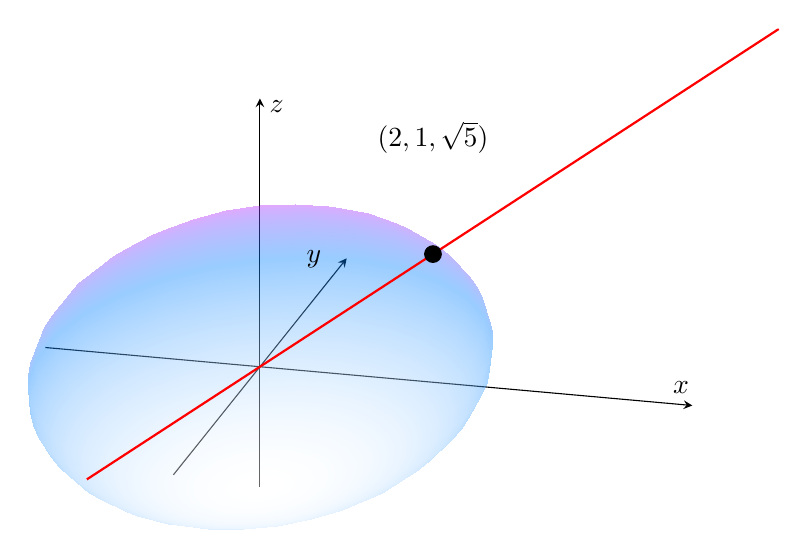
\begin{tikzpicture}
  \begin{axis}[
      view={15}{30},
      axis lines=center,
      xlabel={$x$},
      ylabel={$y$},
      zlabel={$z$},
      width=12cm,
      height=10cm,
      ticks=none,
    ]

    % Plot the sphere x^2 + y^2 + z^2 = R^2
    \addplot3[
      surf,
      opacity=0.4,
      samples=30,
      samples y=30,
      domain=0:360,
      y domain=0:180,
      shader=interp,
      colormap/cool
    ]
    ({3*cos(x)*sin(y)}, {3*sin(x)*sin(y)}, {3*cos(y)});

    % Tangent line at point (2, 1, sqrt(5))
    % Direction vector from gradient: (4, 2, 2sqrt(5))
    \addplot3[
      thick,
      color=red,
      domain=-1:1
    ]
    ({2 + 4*x}, {1 + 2*x}, {2.236 + 2.236*2*x}); % sqrt(5) ≈ 2.236

    % Mark the point of tangency
    \addplot3[
      only marks,
      mark=*,
      mark size=3pt,
      color=black
    ]
    coordinates {(2, 1, 2.236)}; % sqrt(5) ≈ 2.236
    
    % Add labels
    \node at (axis cs:2,1,4.5) [anchor=south] {\( (2, 1, \sqrt{5}) \)};

  \end{axis}
\end{tikzpicture}
\caption{\textit{A normal line to the sphere \(x^2 + y^2 + z^2 = 9\) at the point \((2, 1, \sqrt{5})\). The normal line is shown in red. The point is marked in black.}}

\end{figure}


\noindent This generalization of implicit differentiation highlights the power of the Chain Rule in understanding complex interdependencies among variables, bridging concepts from calculus to more advanced topics in analysis and applied mathematics.


\exampleline
\begin{example}
For the implicit function \( F(x, y, z) = x^2y + yz + e^z = 10 \), where \( z \) is a function of \( x \) and \( y \), find \( \frac{\partial z}{\partial x} \) and \( \frac{\partial z}{\partial y} \).

\begin{solution}
Differentiate both sides of the equation \( F(x, y, z) = 10 \) with respect to \( x \), treating \( z \) as a function of \( x \) and \( y \):
\[
\frac{\partial}{\partial x} \big(x^2y + yz + e^z\big) = \frac{\partial}{\partial x}(10).
\]

Applying the chain rule:
\[
\frac{\partial}{\partial x}(x^2y) + \frac{\partial}{\partial x}(yz) + \frac{\partial}{\partial x}(e^z) = 0.
\]

Compute each term:
\[
\frac{\partial}{\partial x}(x^2y) = 2xy, \quad \frac{\partial}{\partial x}(yz) = y \frac{\partial z}{\partial x}, \quad \frac{\partial}{\partial x}(e^z) = e^z \frac{\partial z}{\partial x}.
\]

Combine the terms:
\[
2xy + y \frac{\partial z}{\partial x} + e^z \frac{\partial z}{\partial x} = 0.
\]

Group terms involving \( \frac{\partial z}{\partial x} \):
\[
\left(y + e^z\right) \frac{\partial z}{\partial x} = -2xy.
\]

Solve for \( \frac{\partial z}{\partial x} \):
\[
\frac{\partial z}{\partial x} = \frac{-2xy}{y + e^z}, \quad \text{provided } y + e^z \neq 0.
\]

Now differentiate \( F(x, y, z) \) with respect to \( y \):
\[
\frac{\partial}{\partial y} \big(x^2y + yz + e^z\big) = \frac{\partial}{\partial y}(10).
\]

Applying the chain rule:
\[
\frac{\partial}{\partial y}(x^2y) + \frac{\partial}{\partial y}(yz) + \frac{\partial}{\partial y}(e^z) = 0.
\]

Compute each term:
\[
\frac{\partial}{\partial y}(x^2y) = x^2, \quad \frac{\partial}{\partial y}(yz) = z + y \frac{\partial z}{\partial y}, \quad \frac{\partial}{\partial y}(e^z) = e^z \frac{\partial z}{\partial y}.
\]

Combine the terms:
\[
x^2 + z + \left(y + e^z\right) \frac{\partial z}{\partial y} = 0.
\]

Group terms involving \( \frac{\partial z}{\partial y} \):
\[
\left(y + e^z\right) \frac{\partial z}{\partial y} = -x^2 - z.
\]

Solve for \( \frac{\partial z}{\partial y} \):
\[
\frac{\partial z}{\partial y} = \frac{-x^2 - z}{y + e^z}, \quad \text{provided } y + e^z \neq 0.
\]
\end{solution}
\end{example}
\exampleline


\subsection*{Total Differentials} \index{Total Differentials}

\noindent The concept of total differentials arises naturally when we want to understand how a multivariable function changes in response to small changes in its inputs. For a single-variable function \( y = f(x) \), the differential \( dy = f'(x) dx \) provides a linear approximation to the change in \( y \). Similarly, for a multivariable function \( w = f(x_1, x_2, \ldots, x_n) \), the total differential \( dw \) captures the combined effect of infinitesimal changes in all input variables:
\[
dw = \sum_{i=1}^n \frac{\partial f}{\partial x_i} dx_i.
\]

\noindent Why focus on \( dw \)? The total differential is not just a mathematical curiosity—it is a powerful tool for estimating the change in \( w \) based on the rates of change (\( \frac{\partial f}{\partial x_i} \)) and the input variations (\( dx_i \)). It provides a linear approximation that simplifies analysis in scenarios where changes in variables are small but interdependent. For example:
\begin{itemize}
    \item In \textbf{error propagation}, \( dw \) quantifies how uncertainties in measurements of \( x_1, x_2, \ldots, x_n \) affect the overall uncertainty in \( w \).
    \item In \textbf{optimization}, \( dw \) aids in understanding the sensitivity of a function to changes in its variables, guiding decisions about which factors matter most.
    \item In \textbf{differential geometry}, \( dw \) generalizes to describe changes on curved surfaces and manifolds, forming the backbone of advanced calculus.
\end{itemize}

\noindent By combining the effects of individual variables into one expression, the total differential serves as a concise and unified way to understand the behavior of multivariable functions in the context of infinitesimal changes.


\exampleline
\begin{example}
The temperature \( T \) at a point in space is given by \( T(x, y, z) = 100 - 2x^2 - y^2 - z^2 \), where \( x, y, z \) are measured in meters. Suppose a sensor moves from the point \( (1, 2, -1) \) to a nearby point \( (1.02, 1.98, -1.01) \). Use the total differential to estimate the change in temperature \( \Delta T \).

\begin{solution}
First, compute the partial derivatives of \( T(x, y, z) \):
\[
\frac{\partial T}{\partial x} = -4x, \quad \frac{\partial T}{\partial y} = -2y, \quad \frac{\partial T}{\partial z} = -2z.
\]

At the point \( (1, 2, -1) \), evaluate these partial derivatives:
\[
\frac{\partial T}{\partial x} = -4(1) = -4, \quad \frac{\partial T}{\partial y} = -2(2) = -4, \quad \frac{\partial T}{\partial z} = -2(-1) = 2.
\]

The total differential \( dT \) is given by:
\[
dT = \frac{\partial T}{\partial x} dx + \frac{\partial T}{\partial y} dy + \frac{\partial T}{\partial z} dz.
\]

Substitute \( dx = 1.02 - 1 = 0.02 \), \( dy = 1.98 - 2 = -0.02 \), and \( dz = -1.01 - (-1) = -0.01 \):
\[
dT = (-4)(0.02) + (-4)(-0.02) + (2)(-0.01).
\]

Simplify:
\[
dT = -0.08 + 0.08 - 0.02 = -0.02.
\]

Thus, the estimated change in temperature is:
\[
\Delta T \approx -0.02 \, \text{°C}.
\]
\end{solution}
\end{example}
\exampleline

\subsection*{Leibniz Integral Rule} \index{Leibniz Integral Rule}

\noindent The Leibniz integral rule extends the utility of the Chain Rule to integrals where the limits of integration or the integrand itself depend on a variable. For a function \( f(x, t) \), consider the integral:
\[
F(x) = \int_{a(x)}^{b(x)} f(x, t) \, dt.
\]
The derivative of \( F(x) \) with respect to \( x \) is given by:
\[
\frac{dF}{dx} = f(x, b(x)) \frac{db}{dx} - f(x, a(x)) \frac{da}{dx} + \int_{a(x)}^{b(x)} \frac{\partial f}{\partial x}(x, t) \, dt,
\]
provided that \( f \) and its partial derivative \( \frac{\partial f}{\partial x} \) are continuous on the region of integration.

\noindent This formula encapsulates three contributions to the rate of change of \( F(x) \):
\begin{itemize}
    \item The first term accounts for the upper limit \( b(x) \) changing, weighted by the value of the integrand \( f(x, t) \) at that limit.
    \item The second term accounts for the lower limit \( a(x) \) changing, weighted by the value of \( f(x, t) \) at that limit.
    \item The third term represents the direct contribution from the dependence of \( f(x, t) \) on \( x \), integrated over the interval.
\end{itemize}

\noindent The Leibniz rule is particularly valuable in applications such as:
\begin{itemize}
    \item Evaluating parametric integrals where the limits or integrand depend on parameters.
    \item Deriving equations in physics and engineering, such as time-dependent conservation laws.
    \item Analyzing probability distributions with varying bounds.
\end{itemize}

\noindent This result demonstrates the interplay between differentiation and integration in multivariable contexts, leveraging the Chain Rule to account for variable dependencies within the integral. 



\newpage

\lecture{Directional Derivatives and Gradient Vectors} \index{Directional Derivatives}

\noindent In previous lectures, we explored the foundational theories of change, including partial derivatives, total differentials, and the Chain Rule. These tools provided insight into how functions change with respect to individual variables or interconnected variables. However, real-world scenarios rarely involve changes along axes alone. Instead, we often need to understand how a function changes in any arbitrary direction in space. This lecture introduces directional derivatives and gradient vectors, which extend the ideas of partial derivatives and total differentials to arbitrary directions. These tools are critical in understanding rates of change, optimizing functions, and impressing your friends who peer over your shoulder with some of the intense notation we are about to partake.

\subsection*{Directional Derivatives} \index{Directional Derivatives}

\noindent The directional derivative quantifies the rate of change of a function \( f(x, y, z) \) in a specific direction. To motivate its introduction, consider the limitations of partial derivatives: they only describe the rate of change of a function along coordinate axes. But what if we are interested in how \( f \) changes in a diagonal direction, or along an arbitrary path? In real-world applications, such as physics or optimization, understanding how a function changes in any given direction is often critical. This leads naturally to the need for directional derivatives.

\noindent Ponder for a moment: if we know how \( f \) changes along the \( x \)-, \( y \)-, and \( z \)-axes, can we combine this information to understand how \( f \) changes in an arbitrary direction? This question guides us toward the definition of the directional derivative. \\

\noindent Consider a function \( f \) defined in \( \mathbb{R}^n \) and a unit vector \( \mathbf{u} \) indicating the direction of interest. The directional derivative of \( f \) at a point \( \mathbf{p} = (x_1, x_2, \ldots, x_n) \) in the direction of \( \mathbf{u} \) is denoted \( D_{\mathbf{u}} f(\mathbf{p}) \) and is defined by equipping our increment $h$ in our usual limit definition of derivative with the direction $\mathbf{u}$:
\[
D_{\mathbf{u}} f(\mathbf{p}) = \lim_{h \to 0} \frac{f(\mathbf{p} + h \mathbf{u}) - f(\mathbf{p})}{h}.
\]

\noindent This definition generalizes the concept of partial derivatives. The numerator, \( f(\mathbf{p} + h \mathbf{u}) - f(\mathbf{p}) \), represents the change in \( f \) as we move from \( \mathbf{p} \) along the direction of \( \mathbf{u} \) by a small distance \( h \). Dividing by \( h \) gives the average rate of change over this small interval, and the limit ensures that we measure the instantaneous rate of change. Let's carefully unpack this definition with an example of notation:
\[
D_{\mathbf{u}} f(\mathbf{p}) = \frac{d}{dh} f(\mathbf{p} + h \mathbf{u}) \bigg|_{h=0}.
\]
Here, the notation \( \mathbf{p} + h \mathbf{u} \) emphasizes that we are moving from \( \mathbf{p} \) in the direction \( \mathbf{u} \), scaled by a small step \( h \). Differentiating with respect to \( h \) isolates the contribution of the directional movement along \( \mathbf{u} \), allowing us to quantify how \( f \) changes specifically due to this displacement. While the definition above is mathematically rigorous, it can be challenging to compute in practice due to the dependency of \( f \) on multiple variables and the complexity of evaluating the limit as \( h \to 0 \). For example, if \( f(x, y) = e^{x^2 + y^2} \) and \( \mathbf{u} = \begin{bmatrix} \frac{\sqrt{2}}{2} \\ \frac{\sqrt{2}}{2} \end{bmatrix} \), we need to evaluate:
\[
f(\mathbf{p} + h \mathbf{u}) = f\left(\begin{bmatrix} p_x + \frac{h \sqrt{2}}{2} \\ p_y + \frac{h \sqrt{2}}{2} \end{bmatrix}\right) = e^{\left(p_x + \frac{h \sqrt{2}}{2}\right)^2 + \left(p_y + \frac{h \sqrt{2}}{2}\right)^2}.
\]
Expanding this expression and differentiating with respect to \( h \) involves tedious calculations that are prone to error.


\begin{figure}[H]
\centering
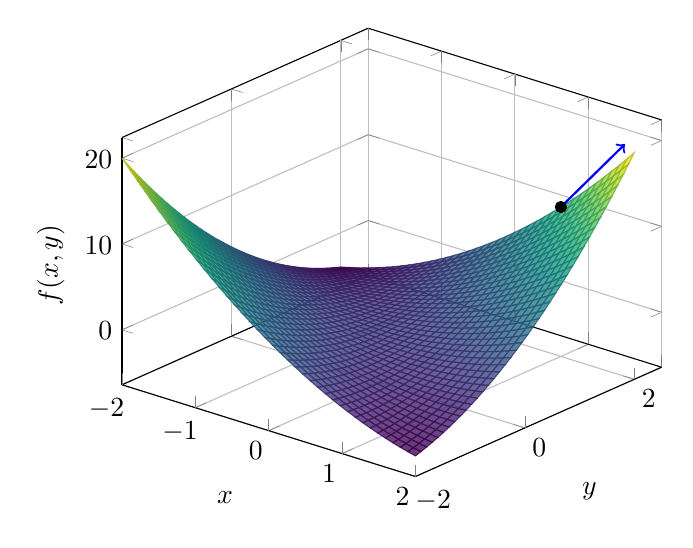
\begin{tikzpicture}
  \begin{axis}[
    view={40}{30},
    xlabel={$x$},
    ylabel={$y$},
    zlabel={$f(x, y)$},
    domain=-2:2,
    y domain=-2:2,
    samples=40,
    samples y=40,
    grid=major,
    colormap/viridis
  ]
    % Plot the surface f(x, y)
    \addplot3[surf,opacity=0.8]
      {x^2 + 3*x*y + y^2};

    % Point of interest \mathbf{p} = (1, 2)
    \addplot3[
      mark=*]
      coordinates {(1, 2, 11)};

    % Directional vector in the direction of \mathbf{u}
    \addplot3[->,thick,blue]
      coordinates {(1, 2, 11) (1.5, 2.5, 18.25)};

  \end{axis}
\end{tikzpicture}
\caption{\textit{A 3D visualization of the function \( f(x, y) = x^2 + 3xy + y^2 \). The point \( \mathbf{p} = (1, 2) \) is marked on the surface, and the blue arrow represents movement in the direction of the unit vector \( \mathbf{u} = \frac{1}{\sqrt{2}} \begin{bmatrix} 1 \\ 1 \end{bmatrix} \), illustrating the directional derivative at \( \mathbf{p} \).}}
\end{figure}


\subsection*{The Gradient Vector} \index{Gradient Vector}

\noindent To fully understand directional derivatives, we must first introduce the gradient vector, a fundamental concept that encapsulates how a function \( f \) changes in all coordinate directions simultaneously. The gradient vector provides the foundation upon which the directional derivative is built. \\

\noindent The gradient of a function \( f \), denoted \( \nabla f \), is a \textit{vector field} that encodes the partial derivatives of \( f \) with respect to each variable. Formally, for \( f: \mathbb{R}^n \to \mathbb{R} \), the gradient vector at a point \( \mathbf{p} = (x_1, x_2, \ldots, x_n) \) is defined as:

\[
\nabla f(\mathbf{p}) = \begin{bmatrix} 
\frac{\partial f}{\partial x_1}(\mathbf{p}) \\[1em] 
\frac{\partial f}{\partial x_2}(\mathbf{p}) \\[1em] 
\vdots \\[1em] 
\frac{\partial f}{\partial x_n}(\mathbf{p}) 
\end{bmatrix}.
\]

\noindent Each component \( \frac{\partial f}{\partial x_i}(\mathbf{p}) \) measures how \( f \) changes as \( x_i \) varies, while all other variables are held constant. Thus, the gradient vector consolidates all partial derivatives into a single geometric entity, pointing in the direction of the steepest ascent of \( f \). Let's knock out a quick example before we continue:


\exampleline
\begin{example}
Compute the gradient vector \( \nabla f \) for the function \( f(x, y, z) = x^2y + yz^3 - \sin(xz) \) at the point \( \mathbf{p} = (1, 2, 0) \).

\begin{solution}
The gradient vector is defined as $\nabla f(x, y, z) = \langle f_x,f_y,f_z \rangle$

Compute each partial derivative:
\begin{itemize}
    \item \( \frac{\partial f}{\partial x} = \frac{\partial}{\partial x} \left( x^2y + yz^3 - \sin(xz) \right) = 2xy - z\cos(xz). \)
    \item \( \frac{\partial f}{\partial y} = \frac{\partial}{\partial y} \left( x^2y + yz^3 - \sin(xz) \right) = x^2 + z^3. \)
    \item \( \frac{\partial f}{\partial z} = \frac{\partial}{\partial z} \left( x^2y + yz^3 - \sin(xz) \right) = 3yz^2 - x\cos(xz). \)
\end{itemize}

Evaluate at \( \mathbf{p} = (1, 2, 0) \):
\begin{itemize}
    \item \( \frac{\partial f}{\partial x}(1, 2, 0) = 2(1)(2) - 0\cos(1 \cdot 0) = 4. \)
    \item \( \frac{\partial f}{\partial y}(1, 2, 0) = (1)^2 + (0)^3 = 1. \)
    \item \( \frac{\partial f}{\partial z}(1, 2, 0) = 3(2)(0)^2 - 1\cos(1 \cdot 0) = -1. \)
\end{itemize}

Thus, the gradient vector at \( \mathbf{p} = (1, 2, 0) \) is:
\[
\nabla f(1, 2, 0) = \begin{bmatrix} 4 \\ 1 \\ -1 \end{bmatrix}.
\]
\end{solution}
\end{example}
\exampleline



\noindent With the gradient in hand, we can rigorously define the directional derivative. The directional derivative \( D_{\mathbf{u}} f(\mathbf{p}) \) quantifies the rate of change of \( f \) at \( \mathbf{p} \) in the direction of a unit vector \( \mathbf{u} \). It is given by:
\[
D_{\mathbf{u}} f(\mathbf{p}) = \nabla f(\mathbf{p}) \cdot \mathbf{u}.
\]

\noindent This equivalence arises because \( \nabla f(\mathbf{p}) \) encapsulates all partial derivatives of \( f \) at \( \mathbf{p} \), and the dot product with \( \mathbf{u} \) effectively weights these partial derivatives according to the components of \( \mathbf{u} \). Specifically, starting from the definition of the directional derivative:
\[
D_{\mathbf{u}} f(\mathbf{p}) = \frac{d}{dh} f(\mathbf{p} + h\mathbf{u}) \bigg|_{h=0},
\]
we recognize that \( \mathbf{p} + h\mathbf{u} \) represents a small displacement from \( \mathbf{p} \) in the direction of \( \mathbf{u} \). Differentiating \( f(\mathbf{p} + h\mathbf{u}) \) with respect to \( h \) involves the chain rule, yielding:
\[
\frac{d}{dh} f(\mathbf{p} + h\mathbf{u}) \bigg|_{h=0} = \nabla f(\mathbf{p}) \cdot \mathbf{u}.
\]
Here, the gradient \( \nabla f(\mathbf{p}) \) acts as a vector of sensitivities, and the dot product projects it onto the direction \( \mathbf{u} \), isolating the rate of change along that direction. \\


\noindent To summarize the formula $D_{\mathbf{u}} f(\mathbf{p}) = \nabla f(\mathbf{p}) \cdot \mathbf{u}$:
\begin{itemize}
    \item The gradient \( \nabla f(\mathbf{p}) \) encapsulates how \( f \) changes in all coordinate directions.
    \item The dot product \( \nabla f(\mathbf{p}) \cdot \mathbf{u} \) projects the gradient onto the direction \( \mathbf{u} \), isolating the rate of change along that direction.
\end{itemize}

\noindent Rewriting the directional derivative in expanded form reveals its structure explicitly:
\[
D_{\mathbf{u}} f(\mathbf{p}) = \nabla f(\mathbf{p}) \cdot \mathbf{u} = \frac{\partial f}{\partial x_1} u_1 + \frac{\partial f}{\partial x_2} u_2 + \cdots + \frac{\partial f}{\partial x_n} u_n = \sum_{i} f_{x_i} u_i,
\]
where \( \mathbf{u} = [u_1, u_2, \ldots, u_n]^T \). This expression shows that the directional derivative is a weighted sum of the partial derivatives, with the weights provided by the components of \( \mathbf{u} \).

\exampleline
\begin{example}
Let \( f(x, y) = x^2 + 3xy + y^2 \), and consider the point \( \mathbf{p} = (1, 2) \) and the unit vector \( \mathbf{u} = \frac{1}{\sqrt{2}} \begin{bmatrix} 1 \\ 1 \end{bmatrix} \). Verify that the directional derivative \( D_{\mathbf{u}} f(\mathbf{p}) \) computed using:
\[
D_{\mathbf{u}} f(\mathbf{p}) = \nabla f(\mathbf{p}) \cdot \mathbf{u},
\]
is the same as:
\[
\frac{d}{dh} f(\mathbf{p} + h \mathbf{u}) \bigg|_{h=0}.
\]

\begin{solution} \\
Step 1: Compute \( D_{\mathbf{u}} f(\mathbf{p}) \) using the gradient and dot product.
\begin{itemize}
    \item The gradient of \( f(x, y) \) is:
    \[
    \nabla f(x, y) = \begin{bmatrix} 2x + 3y \\ 3x + 2y \end{bmatrix}.
    \]
    At \( \mathbf{p} = (1, 2) \):
    \[
    \nabla f(1, 2) = \begin{bmatrix} 2(1) + 3(2) \\ 3(1) + 2(2) \end{bmatrix} = \begin{bmatrix} 8 \\ 7 \end{bmatrix}.
    \]

    \item Compute the dot product:
    \[
    D_{\mathbf{u}} f(\mathbf{p}) = \nabla f(\mathbf{p}) \cdot \mathbf{u} = \begin{bmatrix} 8 \\ 7 \end{bmatrix} \cdot \frac{1}{\sqrt{2}} \begin{bmatrix} 1 \\ 1 \end{bmatrix} = \frac{8 + 7}{\sqrt{2}} = \frac{15}{\sqrt{2}}.
    \]
\end{itemize}

Step 2: Compute \( D_{\mathbf{u}} f(\mathbf{p}) \) using the limit definition.
\begin{itemize}
    \item Substitute \( \mathbf{p} + h \mathbf{u} \) into \( f(x, y) \):
    \[
    f(\mathbf{p} + h \mathbf{u}) = f\left( 1 + \frac{h}{\sqrt{2}}, 2 + \frac{h}{\sqrt{2}} \right).
    \]
    Expand \( f(x, y) = x^2 + 3xy + y^2 \):
    \[
    f\left( 1 + \frac{h}{\sqrt{2}}, 2 + \frac{h}{\sqrt{2}} \right) = \left(1 + \frac{h}{\sqrt{2}}\right)^2 + 3\left(1 + \frac{h}{\sqrt{2}}\right)\left(2 + \frac{h}{\sqrt{2}}\right) + \left(2 + \frac{h}{\sqrt{2}}\right)^2.
    \]
    Combine terms (constant, linear, and quadratic in \( h \)):
    \[
    f(\mathbf{p} + h \mathbf{u}) = 11 + \frac{15h}{\sqrt{2}} + \frac{5h^2}{2}.
    \]

    \item Compute the derivative with respect to \( h \) and evaluate at \( h = 0 \):
    \[
    \frac{d}{dh} f(\mathbf{p} + h\mathbf{u}) = \frac{15}{\sqrt{2}} + 5h.
    \]
    At \( h = 0 \):
    \[
    \frac{d}{dh} f(\mathbf{p} + h \mathbf{u}) \bigg|_{h=0} = \frac{15}{\sqrt{2}}.
    \]
\end{itemize}

Thus, both methods yield \( D_{\mathbf{u}} f(\mathbf{p}) = \frac{15}{\sqrt{2}} \), confirming the equivalence.
\end{solution}
\end{example}
\exampleline


\noindent A natural question arises: why must \( \mathbf{u} \) be a unit vector? The unit length ensures that \( D_{\mathbf{u}} f(\mathbf{p}) \) measures the rate of change per unit distance traveled along \( \mathbf{u} \). If \( \mathbf{u} \) is not a unit vector, the directional derivative would also reflect the scaling of \( \mathbf{u} \), distorting its geometric interpretation. The gradient vector not only simplifies computations but also provides profound geometric insights. Key properties of the gradient include:
\begin{itemize}
    \item \textbf{Direction of Maximum Increase:} The gradient vector points in the direction where \( f \) increases most rapidly. This follows from the dot product \( \nabla f(\mathbf{p}) \cdot \mathbf{u} \), which achieves its maximum value when \( \mathbf{u} \) is aligned with \( \nabla f(\mathbf{p}) \).
    \item \textbf{Magnitude as Rate of Change:} The magnitude \( |\nabla f(\mathbf{p})| \) represents the maximum rate of change of \( f \) at \( \mathbf{p} \).
    \item \textbf{Orthogonality to Level Surfaces:} The gradient is perpendicular to level curves (in two dimensions) or level surfaces (in three dimensions). For example, if \( f(x, y, z) = c \) defines a level surface, then \( \nabla f \) satisfies:
    \[
    \nabla f \cdot \mathbf{v} = 0,
    \]
    where \( \mathbf{v} \) is any tangent vector to the level surface.
\end{itemize}



\noindent Now that we have established the gradient, we can revisit the directional derivative from a conceptual standpoint. The gradient encapsulates all partial derivatives and provides the tools to compute how \( f \) changes along any direction. The directional derivative extends the idea of partial derivatives by generalizing the rate of change from axis-aligned directions to arbitrary directions. This interplay between the gradient and directional derivatives reflects the power and elegance of multivariable calculus, connecting geometry, algebra, and analysis. \\

\noindent The utility of these concepts will become increasingly evident as we apply them to rate-of-change problems, optimization, and the study of vector fields. The gradient, in particular, acts as a bridge between local behavior (how \( f \) changes at a point) and global phenomena (how \( f \) behaves across its entire domain).


\subsection*{Applications to Rate of Change Problems} \index{Rate of Change}

\noindent The concepts of directional derivatives and gradients extend naturally to solving real-world problems involving rates of change. Consider the following scenarios:
\begin{itemize}
    \item \textbf{Temperature Distribution:} In a three-dimensional temperature field \( T(x, y, z) \), the gradient \( \nabla T \) indicates the direction in which temperature increases most rapidly. The magnitude of \( \nabla T \) gives the rate of temperature change in that direction.
    \item \textbf{Flow Problems:} In fluid dynamics, the gradient of a scalar field such as pressure or density can describe the force acting on a fluid particle, guiding its motion.
    \item \textbf{Optimization:} By identifying points where \( \nabla f = 0 \), we can find critical points that are potential extrema or saddle points of the function \( f \). The directional derivative allows us to analyze changes in any desired direction, facilitating a deeper understanding of the function's behavior.
\end{itemize}


\subsubsection*{Gradient Ascent/Descent} \index{Gradient Ascent} \index{Gradient Descent}

\noindent Gradient ascent/descent is a fundamental technique used to navigate scalar fields and locate points of maximum or minimum value by following the direction of steepest ascent or descent. At each point on the scalar field \( f(x, y) \), the gradient vector \( \nabla f \) provides the direction in which \( f \) increases most rapidly. The ascent/descent process is iterative, with each step determined by moving along the gradient direction to transition from one level curve to the next. This section explains how to compute the step vectors \( \mathbf{r} \), which guide this process using the unit vector method.

\begin{enumerate}
    \item \textbf{Understand the Role of the Gradient:}
    The gradient vector \( \nabla f(x, y) = \langle f_x,f_y \rangle \) points in the direction of maximum increase of the function \( f(x, y) \). Its magnitude \( |\nabla f| \) reflects the steepness of the ascent at a point.

    \item \textbf{Define a Step Vector \( \mathbf{r} \) Using a Unit Vector:}
    To ensure consistent step sizes regardless of the gradient's magnitude, define the step vector using a unit vector in the desired direction (ascent or descent):
    \[
    \hat{\mathbf{u}} = \frac{\nabla f(x, y)}{|\nabla f(x, y)|}.
    \]
    This unit vector \( \hat{\mathbf{u}} \) maintains the direction of steepest ascent while standardizing the step's magnitude. The step vector \( \mathbf{r} \) is then given by:
    \[
    \mathbf{r} = \Delta t \cdot \hat{\mathbf{u}},
    \]
    where \( \Delta t \) is a step size parameter that controls the distance moved in the gradient direction.

    \item \textbf{Orienting the Gradient Vector:}
    Depending on whether you aim to perform gradient ascent or gradient descent, orient the gradient vector appropriately by adjusting its sign:
    \begin{itemize}
        \item \textbf{Gradient Ascent:} Use the gradient vector \( \nabla f \) directly to ascend towards higher function values.
        \item \textbf{Gradient Descent:} Use the negative gradient vector \( -\nabla f \) to descend towards lower function values.
    \end{itemize}
    By orienting the gradient vector in the desired direction, the step vector \( \mathbf{r} \) guides the ascent or descent process accordingly.

    \item \textbf{Update the Point of Interest:}
    Starting from a current point \( \mathbf{P}_n = (x_n, y_n) \), compute the next point \( \mathbf{P}_{n+1} \) using:
    \[
    \mathbf{P}_{n+1} = \mathbf{P}_n + \mathbf{r}.
    \]
    This equation updates the position by adding the step vector \( \mathbf{r} \) to the current coordinates of \( \mathbf{P}_n \).

    \item \textbf{Iterate the Ascent/Descent:}
    At \( \mathbf{P}_{n+1} \), recompute the gradient \( \nabla f(\mathbf{P}_{n+1}) \) and determine the next step vector \( \mathbf{r} \). Repeat the process to continue moving upward (ascent) or downward (descent) along the gradient direction. The iterations trace a path of steepest ascent or descent on the scalar field.

    \item \textbf{Connecting to Level Curves:} \index{Level Curves}
    Each point along the ascent/descent path corresponds to a different level curve, defined by \( f(x, y) = c \). The ascent/descent process transitions from one level curve to the next, with the gradient at each point providing the direction of movement. The step vector \( \mathbf{r} \) guides this transition, and its length is determined by the step size \( \Delta t \).

    \item \textbf{Geometric Interpretation:}
    The ascent/descent path is a curve that moves orthogonal to level curves, following the direction of maximum increase or decrease at each step. The vectors \( \mathbf{r} \) represent the incremental displacements along this path, combining direction (from \( \nabla f \) or \( -\nabla f \)) and magnitude (scaled by \( \Delta t \)).

    \item \textbf{Practical Considerations:}
    While \( \Delta t \) determines the step size, its choice affects both the resolution and speed of the ascent/descent. A small \( \Delta t \) provides finer control and accuracy, while a larger \( \Delta t \) speeds up the process but may overshoot critical points or reduce precision.
\end{enumerate}

\noindent Gradient ascent/descent leverages the mathematical properties of the gradient vector to navigate scalar fields systematically. The \( \mathbf{r} \) vectors embody this process by encoding the direction and magnitude of each step. By iteratively computing \( \mathbf{r} \), we construct a path of steepest ascent or descent that traverses successive level curves and approaches points of maximum or minimum value on \( f(x, y) \).


\begin{figure}[H]
\centering
    \begin{tikzpicture}[samples=50,smooth]
            %\clip(-4,-1) rectangle (4,4);
            \path[bend left,name path=arrowcurve] (-2,4) to[out=-30,in=-160] (0,0);
            \foreach \y[count=\i] in {20,16,12,8,4,1,0.0625}{
            \pgfmathsetmacro\colper{\y*4} % color percentage variable
                \draw[name path global/.expanded=curve\i,white!\colper!black] plot[domain=0:360] ({cos(\x)*sqrt(\y/(sin(2*\x)+2))},{sin(\x)*sqrt(\y/(sin(2*\x)+2))});
                \draw[name intersections = {of ={curve\i} and arrowcurve}](intersection-1) coordinate (P\i);
                \ifnum\i=1 
                    % do nothing
                \else%
                    \pgfmathtruncatemacro\imin{\i-1}
                    \pgfmathtruncatemacro\iprint{\i-2}
                    \draw[->, blue, ultra thick] (P\imin) -- (P\i) node[above right,midway] {\scriptsize $\hat{r}_{\iprint}$}; 
                \fi%
            }     
    \end{tikzpicture}
\caption{\textit{An example of gradient ascent on a set of level curves, where $\mathbf{\hat{r}}_i$ indicates the normal vector between level curves.}}
\end{figure}

\exampleline
\begin{example}
Consider the level curves of the function \( f(x, y) = 4 - x^2 - y^2 \), representing concentric circles centered at the origin. Starting at the point \( \mathbf{P}_1 = (0.5, 0.5) \), compute the unit vectors \( \hat{\mathbf{r}}_1 \) and \( \hat{\mathbf{r}}_2 \), which point in the direction of steepest descent toward the center of the level curves as we move to the next two inner level curves.

\begin{solution}
\noindent The gradient vector \( \nabla f(x, y) \) points radially outward, so the negative gradient \( -\nabla f(x, y) \) points inward, toward the center of the level curves. Let's compute \( \hat{\mathbf{r}}_1 \) and \( \hat{\mathbf{r}}_2 \) step by step.

\begin{enumerate}
    \item \textbf{Compute the gradient at \( \mathbf{P}_1 = (0.5, 0.5) \):}
    \[
    \nabla f(x, y) = \begin{bmatrix} \frac{\partial f}{\partial x} \\ \frac{\partial f}{\partial y} \end{bmatrix} = \begin{bmatrix} -2x \\ -2y \end{bmatrix}.
    \]
    At \( \mathbf{P}_1 = (0.5, 0.5) \):
    \[
    \nabla f(0.5, 0.5) = \begin{bmatrix} -1.0 \\ -1.0 \end{bmatrix}.
    \]
    The negative gradient vector is:
    \[
    -\nabla f(0.5, 0.5) = \begin{bmatrix} 1.0 \\ 1.0 \end{bmatrix}.
    \]
    Compute its magnitude:
    \[
    |-\nabla f(0.5, 0.5)| = \sqrt{(1.0)^2 + (1.0)^2} = \sqrt{1 + 1} = \sqrt{2} \approx 1.414.
    \]
    The unit vector pointing toward the center is:
    \[
    \hat{\mathbf{r}}_1 = \frac{-\nabla f(0.5, 0.5)}{|-\nabla f(0.5, 0.5)|} = \frac{1}{1.414} \begin{bmatrix} 1.0 \\ 1.0 \end{bmatrix} \approx \begin{bmatrix} 0.707 \\ 0.707 \end{bmatrix}.
    \]
    (Note: For simplicity in plotting, we've approximated \( \hat{\mathbf{r}}_1 \) to \( (-0.707, -0.707) \), maintaining the direction.)

    \item \textbf{Move to the next points:}
    Starting from \( \mathbf{P}_1 = (0.5, 0.5) \), we move two steps along the direction of \( \hat{\mathbf{r}}_1 \) and \( \hat{\mathbf{r}}_2 \).

    -First Step (\( \mathbf{P}_1 \) to \( \mathbf{P}_2 \)):
      \[
      \mathbf{P}_2 = \mathbf{P}_1 + h \hat{\mathbf{r}}_1 = (0.5, 0.5) + 0.3 \cdot (-0.707, -0.707) = (0.5 - 0.212, 0.5 - 0.212) = (0.29, 0.29)
      \]
      \[
      z_2 = 4 - (0.29)^2 - (0.29)^2 = 4 - 0.0841 - 0.0841 = 3.83
      \]
      Thus, \( \mathbf{P}_2 = (0.29, 0.29, 3.83) \).

    -Second Step (\( \mathbf{P}_2 \) to \( \mathbf{P}_3 \)):
      \[
      \mathbf{P}_3 = \mathbf{P}_2 + h \hat{\mathbf{r}}_2 = (0.29, 0.29) + 0.3 \cdot (-0.707, -0.707) = (0.29 - 0.212, 0.29 - 0.212) = (0.08, 0.08)
      \]
      \[
      z_3 = 4 - (0.08)^2 - (0.08)^2 = 4 - 0.0064 - 0.0064 = 3.99
      \]
      Thus, \( \mathbf{P}_3 = (0.08, 0.08, 3.99) \).

    \item \textbf{Interpretation:}
    Both \( \hat{\mathbf{r}}_1 \) and \( \hat{\mathbf{r}}_2 \) are unit vectors pointing inward, consistent with the symmetry of the concentric level curves. These vectors demonstrate the direction of steepest descent at each step as we move closer to the center of the level curves.
\end{enumerate}

\begin{figure}[H]
\centering
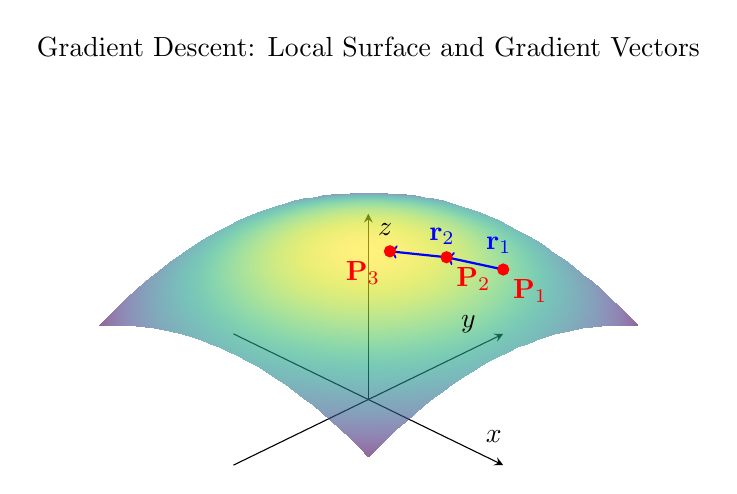
\begin{tikzpicture}
  \begin{axis}[
    view={45}{45}, % Adjust the view angle for better visualization
    xlabel={$x$}, ylabel={$y$}, zlabel={$z$},
    domain=-1:1, % Adjusted domain to focus on relevant region
    y domain=-1:1,
    zmin=0, zmax=5,
    grid=major,
    samples=30,
    samples y=30,
    colormap/viridis,
    title={Gradient Descent: Local Surface and Gradient Vectors},
    axis lines=center,
    ticks=none,
  ]

    % Plot the surface f(x, y) = 4 - x^2 - y^2
    \addplot3[
      surf,
      opacity=0.6,
      shader=interp,
    ] {4 - x^2 - y^2};

    % Plot points P1, P2, and P3 with fixed z-values
    \addplot3[
      only marks,
      mark=*,
      mark size=2pt,
      color=red,
    ] coordinates {
      (0.5, 0.5, 3.5)    % P1
      (0.29, 0.29, 3.83) % P2
      (0.08, 0.08, 3.99) % P3
    };

    % Draw gradient descent vectors from P1 to P2 and P2 to P3
    \addplot3[
      ->,
      thick,
      blue,
    ] coordinates {
      (0.5, 0.5, 3.5)
      (0.29, 0.29, 3.83)
    };

    \addplot3[
      ->,
      thick,
      blue,
    ] coordinates {
      (0.29, 0.29, 3.83)
      (0.08, 0.08, 3.99)
    };

    % Annotate points
    \node[below right, red] at (axis cs:0.5,0.5,3.5) {\( \mathbf{P}_1 \)};
    \node[below right, red] at (axis cs:0.29,0.29,3.83) {\( \mathbf{P}_2 \)};
    \node[below left, red] at (axis cs:0.08,0.08,3.99) {\( \mathbf{P}_3 \)};

    % Label for the gradient vectors
    \node[above right, blue] at (axis cs:0.40,0.40,3.67) {$\mathbf{r}_1$};
    \node[above right, blue] at (axis cs:0.19,0.19,3.91) {$\mathbf{r}_2$};

  \end{axis}
\end{tikzpicture}
\caption{\textit{The gradient descent of the two vectors found in this problem starting at point \( \mathbf{P}_1 = (0.5, 0.5) \).}}
\end{figure}

\end{solution}
\end{example}

\exampleline


\begin{example} 
A room has a temperature distribution given by \( T(x, y, z) = 100 - x^2 - y^2 - z^2 \), where \( T \) is measured in degrees Celsius, and \( x, y, z \) are measured in meters. At the point \( \mathbf{p} = (1, 1, 1) \), find:
\begin{enumerate}
    \item The gradient of \( T \).
    \item The direction of the steepest ascent of the temperature.
    \item The rate of change of the temperature in the direction of the steepest ascent.
\end{enumerate}

\begin{solution}
\noindent The gradient vector is defined as \( \nabla T(x, y, z) = \langle T_x, T_y, T_z \rangle \).

\begin{enumerate}
    \item Compute each partial derivative:
    \begin{itemize}
        \item \( \frac{\partial T}{\partial x} = \frac{\partial}{\partial x} \left( 100 - x^2 - y^2 - z^2 \right) = -2x. \)
        \item \( \frac{\partial T}{\partial y} = \frac{\partial}{\partial y} \left( 100 - x^2 - y^2 - z^2 \right) = -2y. \)
        \item \( \frac{\partial T}{\partial z} = \frac{\partial}{\partial z} \left( 100 - x^2 - y^2 - z^2 \right) = -2z. \)
    \end{itemize}

    At \( \mathbf{p} = (1, 1, 1) \), the gradient is:
    \[
    \nabla T(1, 1, 1) = \begin{bmatrix} -2(1) \\ -2(1) \\ -2(1) \end{bmatrix} = \begin{bmatrix} -2 \\ -2 \\ -2 \end{bmatrix}.
    \]

    \item The direction of the steepest ascent is given by the unit vector in the direction of \( \nabla T(1, 1, 1) \). Compute the magnitude of \( \nabla T(1, 1, 1) \):
    \[
    |\nabla T(1, 1, 1)| = \sqrt{(-2)^2 + (-2)^2 + (-2)^2} = \sqrt{12} = 2\sqrt{3}.
    \]
    The unit vector is:
    \[
    \mathbf{u} = \frac{\nabla T(1, 1, 1)}{|\nabla T(1, 1, 1)|} = \frac{1}{2\sqrt{3}} \begin{bmatrix} -2 \\ -2 \\ -2 \end{bmatrix} = \begin{bmatrix} -\frac{1}{\sqrt{3}} \\ -\frac{1}{\sqrt{3}} \\ -\frac{1}{\sqrt{3}} \end{bmatrix}.
    \]

    \item The rate of change of the temperature in the direction of the steepest ascent is the magnitude of the gradient:
    \[
    |\nabla T(1, 1, 1)| = 2\sqrt{3}.
    \]
    Thus, the steepest ascent occurs in the direction of \( \mathbf{u} \), with a rate of change of \( 2\sqrt{3} \) degrees Celsius per meter.
\end{enumerate}
\end{solution}
\end{example}
\exampleline



\subsubsection{Gradient Descent in Machine Learning}

Gradient descent is a cornerstone optimization algorithm widely used in machine learning to minimize loss functions, thereby improving model accuracy. At its core, gradient descent iteratively adjusts the model's parameters to find the set of values that result in the lowest possible error between the predicted outputs and the actual data. In machine learning, the objective is often to minimize a loss function (also known as a cost function), which quantifies the difference between the model's predictions and the true values. Common examples include Mean Squared Error (MSE) for regression tasks and Cross-Entropy Loss for classification tasks. \\

\noindent Starting with an initial set of parameters \( \theta_0 \) (which can be chosen randomly or based on some heuristic), gradient descent proceeds by computing the gradient of the loss function with respect to each parameter. This gradient indicates the direction of the steepest increase in the loss. To minimize the loss, the algorithm updates each parameter in the opposite direction of the gradient using a unit vector approach:
\[
\hat{\mathbf{u}} = \frac{\nabla_{\theta} L(\theta)}{|\nabla_{\theta} L(\theta)|}
\]
\[
\theta_{\text{new}} = \theta_{\text{old}} - \alpha \cdot \hat{\mathbf{u}}
\]
where:
\begin{itemize}
    \item \( \theta \) represents the model parameters.
    \item \( \alpha \) is the \textbf{learning rate}, a hyperparameter that controls the size of the update steps.
    \item \( \nabla_{\theta} L(\theta) \) is the gradient of the loss function with respect to the parameters.
    \item \( \hat{\mathbf{u}} \) is the \textbf{unit vector} in the direction of the gradient, ensuring consistent step sizes.
\end{itemize}

\noindent The process repeats—computing gradients and updating parameters—until the algorithm converges to a minimum of the loss function. Convergence is typically achieved when changes in the loss function become negligible or after a predefined number of iterations. There are several variants of gradient descent tailored to different scenarios, including Batch Gradient Descent, Stochastic Gradient Descent (SGD), and Mini-Batch Gradient Descent. \\ \\ Gradient descent is favored in machine learning due to its simplicity and efficiency in handling large-scale problems. It scales well with data size and model complexity, making it suitable for training deep neural networks and other complex models. Selecting an appropriate learning rate \( \alpha \) is crucial; a learning rate that is too high can cause the algorithm to overshoot minima, while a rate that is too low can result in slow convergence. Techniques like learning rate scheduling and adaptive learning rate algorithms (e.g., Adam, RMSprop) are often employed to address these challenges. \\

\noindent Gradient descent leverages the mathematical properties of the gradient vector to navigate loss landscapes systematically. The step vectors \( \mathbf{r} \) embody this process by encoding the direction and magnitude of each update. By iteratively computing \( \mathbf{r} \), we construct a path of steepest descent that traverses successive level curves and approaches points of minimum loss on \( f(\theta) \). \\

\noindent The example Python code below minimizes a function, in this case $f(x) = x^2$, from a starting value with a learning rate. Obviously, the minimum of this function is $0$, and we can see that the algorithm is learning its way down to reach that value.

\vspace{1.3em} \index{Python}


\begin{lstlisting}[language=Python]
import numpy as np
import matplotlib.pyplot as plt

def gradient_descent(func, grad_func, initial_x, learning_rate, num_iterations):
    x = initial_x
    x_history = [x]

    for i in range(num_iterations):
        grad = grad_func(x)        # Compute the gradient at current x
        x = x - learning_rate * grad  # Update x in the opposite direction of the gradient
        x_history.append(x)        # Record the new x value

        # Optional: Print progress every 10 iterations
        if (i+1) % 10 == 0:
            print(f"Iteration {i+1}: x = {x:.4f}, f(x) = {func(x):.4f}")

    return x_history

# Example usage with the function f(x) = x^2
def f(x):
    return x**2

def grad_f(x):
    return 2*x

# Parameters for gradient descent
initial_x = 10        # Starting point
learning_rate = 0.1   # Step size
num_iterations = 50   # Number of iterations

# Perform gradient descent
x_history = gradient_descent(f, grad_f, initial_x, learning_rate, num_iterations)

# Plotting the optimization path
iterations = range(len(x_history))
function_values = [f(x) for x in x_history]

plt.figure(figsize=(10, 6))
plt.plot(iterations, function_values, marker='o', linestyle='-', color='b')
plt.title('Gradient Descent Optimization Path')
plt.xlabel('Iteration')
plt.ylabel('f(x) = x^2')
plt.grid(True)
plt.show()
\end{lstlisting}

\vspace{1.3em}

The graph below shows the journey of the gradient descent minimizing $f(x)$.

\begin{figure}[H]
    \centering
    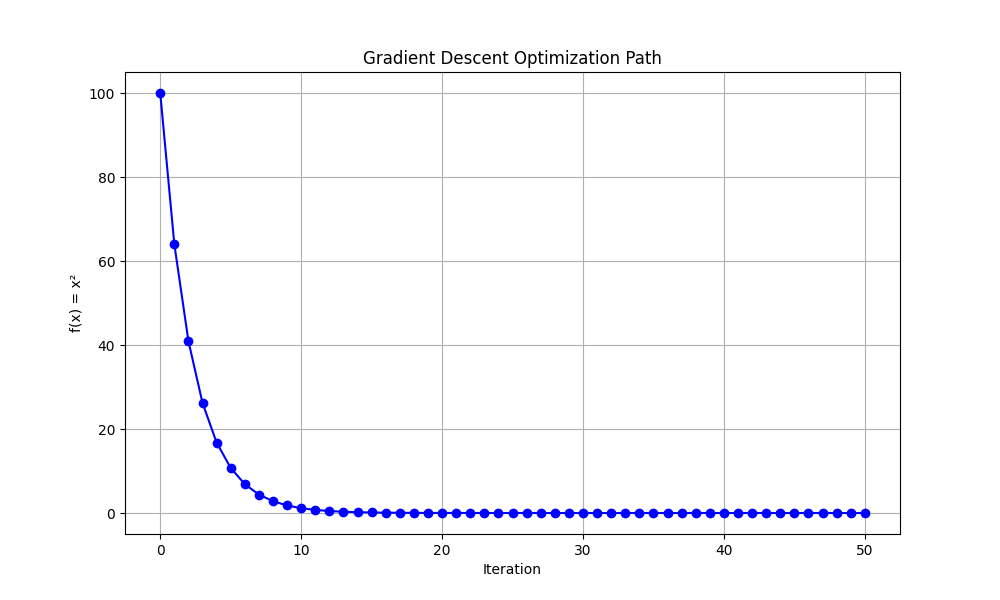
\includegraphics[width=1\textwidth]{chapters/chp3_pics/gd_ex.png}
\caption{\textit{Gradient descent for minimizing the function $f(x) = x^2$}}

    \label{fig:grad_desc_ex}
\end{figure}







\newpage

\lecture{Tangent Planes and Linear Approximations}

\noindent In our exploration of multivariable functions, we have examined how these functions change with respect to their independent variables and how to capture this change using partial derivatives. A central concept in single-variable calculus is the linear approximation of a function near a point, often expressed as the tangent line approximation. In multiple dimensions, the analogous idea is the \textit{tangent plane}, which provides a two-dimensional linear approximation to a surface near a given point. In this lecture, we extend our intuition from single-variable calculus to functions of several variables, focusing on tangent planes and linear approximations. We will also connect these ideas to differentials, which enable us to approximate small changes in a function and apply these approximations to estimate errors in measurements and computations.

\subsection*{From Tangent Lines to Tangent Planes} \index{Tangent Planes}

\noindent Recall from Single-Variable Calculus: you have a function \( y = f(x) \) that is differentiable at a point \( x = a \). If we zoom in very close to the graph of \( f \) at \( (a, f(a)) \), the curve appears almost indistinguishable from a straight line. This line is the \textit{tangent line}, and it gives the best linear approximation to \( f \) near \( x = a \). How do we find this tangent line? We know the slope of the tangent line is given by the derivative \( f'(a) \). The point of tangency is \((a, f(a))\). Combining this information, the equation of the tangent line is:
\[
y \approx f(a) + f'(a)(x - a).
\]

\noindent This linear function approximates \( f(x) \) well for \( x \) near \( a \). In other words, we have a local, linear predictor:
\[
f(x) \approx f(a) + f'(a)(x - a).
\]

\noindent This approximation is not just a convenient guess; it emerges naturally from the definition of the derivative:
\[
f'(a) = \lim_{h \to 0} \frac{f(a+h) - f(a)}{h}.
\]
If we rearrange this definition for small \( h \):
\[
f(a+h) \approx f(a) + f'(a)h,
\]
which is exactly our linear approximation. As \( h \to 0 \), this approximation becomes increasingly accurate. \\

\noindent Now, consider a function of two variables:
\[
z = f(x,y).
\]
We want an analogous concept to the tangent line, but now our domain is two-dimensional, and the graph of \( f \) is a surface in three-dimensional space. Instead of a line, the natural linear approximation to a surface at a given point is a \textit{tangent plane}. \\

\noindent Suppose \( f \) is differentiable at a point \((a,b)\). Differentiability in two dimensions means that as we move from \((a,b)\) to \((a+\Delta x, b+\Delta y)\), the change in \( f \) can be approximated by a linear function of \(\Delta x\) and \(\Delta y\). Let’s express this idea. \\

\noindent In single-variable calculus, differentiability required that:
\[
f(a+h) = f(a) + f'(a)h + \epsilon(h), \quad \text{where } \epsilon(h) \to 0 \text{ as } h \to 0.
\]

\noindent In two-variable calculus, if \( f \) is differentiable at \((a,b)\), we have:
\[
f(a+\Delta x, b+\Delta y) = f(a,b) + f_x(a,b)\Delta x + f_y(a,b)\Delta y + E(\Delta x,\Delta y),
\]
where \( f_x(a,b) \) and \( f_y(a,b) \) are the partial derivatives of \( f \) at \((a,b)\). Here, \(\Delta x\) and \(\Delta y\) are small increments in \( x \) and \( y \) (often denoted by \( h \) and \( k \) in limit definitions). The term \( E(\Delta x,\Delta y) \) is an error term that goes to zero faster than \(\sqrt{(\Delta x)^2 + (\Delta y)^2}\) as \(\Delta x,\Delta y \to 0\). More precisely:
\[
\lim_{(h,k)\to(0,0)} \frac{E(h,k)}{\sqrt{h^2+k^2}} = 0.
\]

\noindent Thus, as \((\Delta x,\Delta y)\) become infinitesimally small, the linear part dominates and the higher-order terms become negligible. This stems from the definition of differentiability, which ensures that the function's behavior is well-approximated by a linear map at the point of tangency.

\begin{figure}[H]
\centering

%---------------------------------------------
% Left figure (Global View):
% To adjust how far the axes extend, you can change the domain for x and y,
% as well as the size of the plot. For instance, 'domain=-3:3' and 'y domain=-3:3'
% control the range of x and y. Also, 'width=7cm, height=7cm' affects the size.
% Increase these values for a bigger view.
%---------------------------------------------
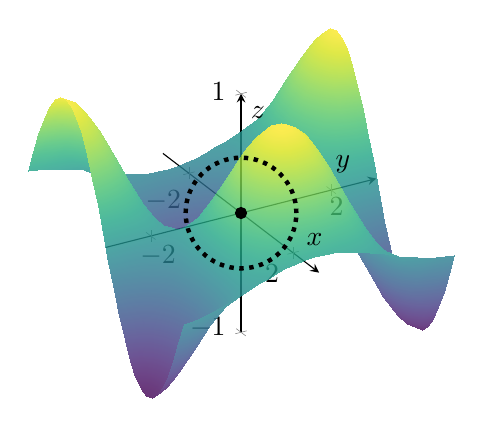
\begin{tikzpicture}
  \begin{axis}[
    width=7cm, height=7cm,         % You can increase these for a bigger plot
    view={60}{30},
    xlabel={$x$}, ylabel={$y$}, zlabel={$z$},
    domain=-3:3, y domain=-3:3,    % Adjust domain range to show more/less of the surface
    samples=30, samples y=30,
    zmin=-1, zmax=1,
    colormap/viridis,
    axis lines=middle,
    grid=major,
    clip=false
  ]
    % Surface: z = sin(x)*cos(y)
    \addplot3[surf, shader=interp, opacity=0.8] {sin(deg(x))*cos(deg(y))};

    % Point of interest (0,0,0)
    \addplot3[mark=*,color=black] coordinates {(0,0,0)};

    % Dotted circle around (0,0)
    \draw[dotted, ultra thick] (axis cs:0,0,0) circle[radius=20pt];

  \end{axis}
\end{tikzpicture}
\hspace{1cm}
%---------------------------------------------
% Right figure (Zoomed-in View):
% Again, to adjust the axes, modify 'domain', 'y domain', and 'width/height'.
% For example, to zoom in more, decrease the domain range; to see more detail, 
% increase samples.
%---------------------------------------------
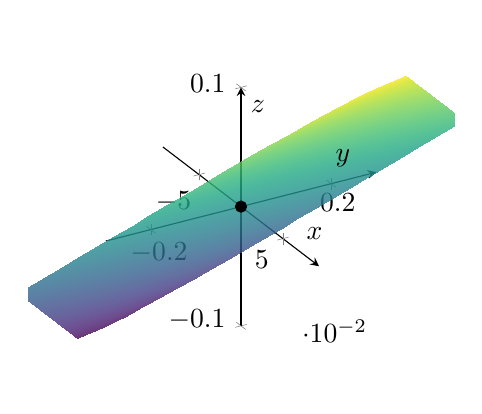
\begin{tikzpicture}
  \begin{axis}[
    width=7cm, height=7cm,         % Increase for a bigger plot if desired
    view={60}{30},
    xlabel={$x$}, ylabel={$y$}, zlabel={$z$},
    domain=-0.3:0.3, y domain=-0.3:0.3,  % Adjust these for how 'zoomed in' the view is
    samples=30, samples y=30,
    zmin=-0.1, zmax=0.1,
    colormap/viridis,
    axis lines=middle,
    grid=major
  ]
    % Surface near (0,0): z=sin(x)*cos(y)
    \addplot3[
      surf,
      shader=interp,
      opacity=0.8
    ] {sin(deg(x))*cos(deg(y))};

    % Point of interest (0,0,0)
    \addplot3[mark=*,color=black] coordinates {(0,0,0)};

  \end{axis}
\end{tikzpicture}

\caption{\textit{Left: A global view of $z=\sin(x)\cos(y)$ with a dotted region around $(0,0)$. 
Right: A zoomed-in view of the same surface near $(0,0)$, where it appears nearly flat.}}
\end{figure}




\noindent Focusing only on the linear part gives:
\[
f(a+\Delta x, b+\Delta y) \approx f(a,b) + f_x(a,b)\Delta x + f_y(a,b)\Delta y.
\]

\noindent Setting \( x = a + \Delta x \) and \( y = b + \Delta y \), we rewrite this as:
\[
f(x,y) \approx f(a,b) + f_x(a,b)(x - a) + f_y(a,b)(y - b).
\]

\noindent This defines a plane:
\[
z = f(a,b) + f_x(a,b)(x - a) + f_y(a,b)(y - b).
\]

Let \( z_0 = f(a,b) \). Then we can rewrite this as:
\[
z - z_0 = f_x(a,b)(x - a) + f_y(a,b)(y - b),
\]
which matches the standard form of a plane equation: a constant point \((a,b,z_0)\) plus linear terms in \((x-a)\) and \((y-b)\). Here, the ``slopes'' \( f_x(a,b) \) and \( f_y(a,b) \) serve as the coefficients that determine the plane’s tilt in the \( x \)- and \( y \)-directions. In other words, this \textbf{tangent plane} at \((a,b,f(a,b))\) just grazes the surface at that point and provides the best linear approximation, making the surface and the plane virtually indistinguishable when we are very close to \((a,b)\). Below we have an example of a plane tangent to a surface:

\noindent This is powerful: it means we can approximate a complicated surface near any point with a simple plane. If we know the function value and its partial derivatives at one point, we can estimate the function at nearby points without recomputing---an idea that underpins error estimation, numerical methods, and optimization.\\ \\

%---------------------------------------------
% Tangent Plane for f(x,y) = x^2 + y^2 at (1,1)
%---------------------------------------------
\begin{figure}[H]
\centering
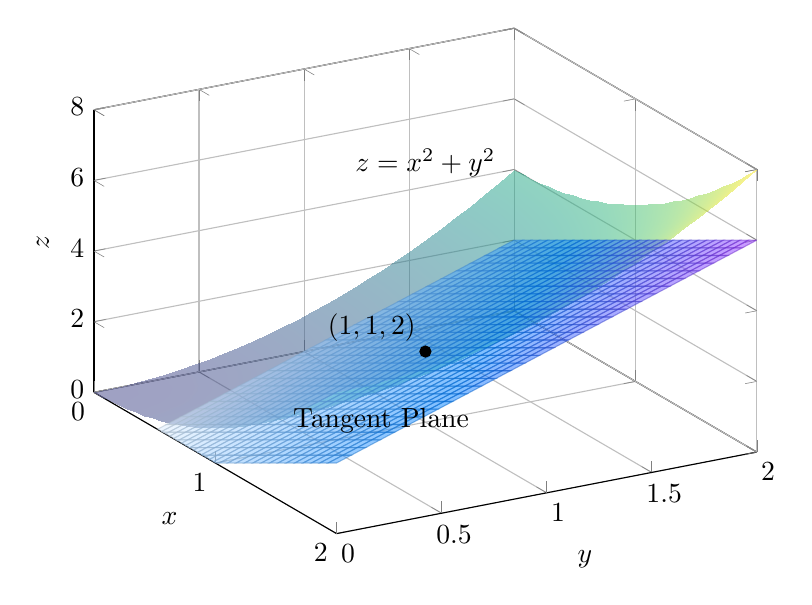
\begin{tikzpicture}
  \begin{axis}[
    view={60}{30},
    xlabel={$x$}, ylabel={$y$}, zlabel={$z$},
    domain=-0.5:2.5,
    y domain=-0.5:2.5,
    samples=30,
    samples y=30,
    width=10cm, height=8cm,
    zmin=0, zmax=8,
    grid=major,
    colormap/viridis,
    ztick={0,2,4,6,8}
  ]

    % Plot the surface f(x,y) = x^2 + y^2
    \addplot3[
      surf,
      opacity=0.5,
      shader=interp,
      domain=0:2,
      y domain=0:2,
    ] {x^2 + y^2};

    % Point of tangency (1,1)
    \addplot3[mark=*,color=black] coordinates {(1,1,2)};

    % Compute tangent plane at (1,1):
    % f_x=2x, f_y=2y at (1,1) => f_x=2, f_y=2
    % f(1,1)=1+1=2
    % Tangent plane: z = 2 + 2(x-1) + 2(y-1) = 2x+2y-2
    \addplot3[
      domain=0:2,
      y domain=0:2,
      surf,
      opacity=0.5,
      colormap/cool,
    ] {2*x+2*y-2};

    % Labels
    \node at (axis cs:1,1,2) [anchor=south east] {$(1,1,2)$};
    \node at (axis cs:1,1,8) [anchor=north] {$z=x^2+y^2$};
    \node at (axis cs:1.5,0.5,1) [anchor=south] {Tangent Plane};
  \end{axis}
\end{tikzpicture}
\caption{\textit{Tangent plane to $z=x^2+y^2$ at the point $(1,1,2)$.}}
\end{figure}

\exampleline
\begin{example}
Find the equation of the tangent plane to the surface
\[
z = f(x,y) = x^2 - 3xy + 4y^2
\]
at the point \((2,1)\).

\begin{solution}
First, we need the partial derivatives of \( f \) with respect to \( x \) and \( y \):
\[
f_x(x,y) = 2x - 3y, \quad f_y(x,y) = -3x + 8y.
\]

Evaluate these at \((2,1)\):
\[
f_x(2,1) = 2(2) - 3(1) = 4 - 3 = 1, \quad f_y(2,1) = -3(2) + 8(1) = -6 + 8 = 2.
\]

Also, find \( f(2,1) \):
\[
f(2,1) = (2)^2 - 3(2)(1) + 4(1)^2 = 4 - 6 + 4 = 2.
\]

The tangent plane is given by:
\[
z = f(2,1) + f_x(2,1)(x - 2) + f_y(2,1)(y - 1).
\]

Substitute the values:
\[
z = 2 + 1(x - 2) + 2(y - 1).
\]

Simplify:
\[
z = 2 + (x - 2) + 2y - 2 = x + 2y - 2.
\]

Thus, the equation of the tangent plane is:
\[
z = x + 2y - 2.
\]
It doesn't get much harder than that!
\end{solution}
\end{example}
\exampleline


\subsection*{Generalization to Higher Dimensions and Hyperplanes} \index{Hyperplanes}

\noindent The concept of tangent planes naturally extends to functions of more than two variables. For a function
\[
f: \mathbb{R}^n \to \mathbb{R},
\]
differentiability at a point \(\mathbf{a} = (a_1, a_2, \ldots, a_n)\) means that we can approximate \( f \) near \(\mathbf{a}\) by a linear function involving the partial derivatives with respect to each of the \( n \) variables. Specifically, we have:
\[
f(\mathbf{a} + \Delta \mathbf{x}) = f(\mathbf{a}) + \nabla f(\mathbf{a}) \cdot \Delta \mathbf{x} + E(\Delta \mathbf{x}),
\]
where \(\nabla f(\mathbf{a})\) is the gradient vector of \( f \) at \(\mathbf{a}\), and \(\Delta \mathbf{x}\) is a small displacement vector in \(\mathbb{R}^n\). Ignoring the small error term, we obtain a linear approximation:
\[
f(\mathbf{a} + \Delta \mathbf{x}) \approx f(\mathbf{a}) + \nabla f(\mathbf{a}) \cdot \Delta \mathbf{x}.
\]

\noindent The set of points \((\mathbf{x}, z)\) in \(\mathbb{R}^{n+1}\) satisfying
\[
z = f(\mathbf{a}) + \nabla f(\mathbf{a}) \cdot (\mathbf{x}-\mathbf{a})
\]
defines a \textit{tangent hyperplane} to the graph of \( f \) at \(\mathbf{a}\). For \( n=1 \), this hyperplane is just a line (the tangent line). For \( n=2 \), it’s a plane (the tangent plane). For \( n>2 \), the object is an \(n\)-dimensional hyperplane—a direct generalization of the idea of “flat” linear approximations to higher dimensions.

\subsubsection*{Hyperplanes in Machine Learning:}  \index{Hyperplanes}
In machine learning, hyperplanes appear in various contexts, notably in classification tasks. For instance, linear classifiers such as Support Vector Machines (SVMs) or simple linear regression models rely on hyperplanes to separate data points or fit data. Consider a binary classification problem in \(\mathbb{R}^n\). A linear classifier tries to find a hyperplane:
\[
\mathbf{w} \cdot \mathbf{x} + b = 0,
\]
that best separates data points of different classes. Here, \(\mathbf{w}\) is a weight vector (analogous to the gradient vector), and \( b \) is a bias term (analogous to a constant offset). The hyperplane defined by this equation divides \(\mathbb{R}^n\) into two half-spaces, and the classifier assigns points on one side to one class and points on the other side to the opposite class. \\

\noindent The connection between the tangent plane (or hyperplane) in calculus and the hyperplanes in machine learning is conceptually significant. Both represent the idea of using linear structures to approximate or make decisions about more complex, nonlinear situations. In calculus, the tangent hyperplane locally approximates a nonlinear function. In machine learning, a hyperplane provides a simple linear boundary in a potentially high-dimensional space. Although the goals differ—approximation of functions vs. classification of points—the underlying mathematical object (a linear function defining a hyperplane) is fundamentally the same.

\subsubsection*{A Simple Linear Classifier in 2D} \index{Linear Classifier}

\noindent Consider a simple binary classification task in two dimensions. Suppose each data point is represented by a vector \(\mathbf{x} = (x_1, x_2)\) in \(\mathbb{R}^2\), and we want to classify it into one of two classes, say ``A" or ``B". A very basic linear classifier can be written as:
\[
\mathbf{w} \cdot \mathbf{x} + b = 0,
\]
where \(\mathbf{w} = (w_1, w_2)\) is a weight vector and \( b \) is a bias term. \\

\noindent This equation defines a line in the \( x_1x_2 \)-plane, which is a 1-dimensional hyperplane (since a line is a hyperplane in \(\mathbb{R}^2\)). The classifier assigns points on one side of the line to class A and points on the other side to class B. Specifically:
\[
\mathbf{w} \cdot \mathbf{x} + b > 0 \implies \text{Class A}, \quad \mathbf{w} \cdot \mathbf{x} + b < 0 \implies \text{Class B}.
\]

\noindent For example, let’s choose \( \mathbf{w} = (1, -2) \) and \( b = 1 \). The decision boundary is:
\[
1 \cdot x_1 + (-2) \cdot x_2 + 1 = 0 \implies x_1 - 2x_2 + 1 = 0.
\]

\noindent Rearranging:
\[
x_1 = 2x_2 - 1.
\]

\noindent This line divides the plane into two regions:
\[
x_1 > 2x_2 - 1 \implies \mathbf{x} \text{ is in Class A}, \quad x_1 < 2x_2 - 1 \implies \mathbf{x} \text{ is in Class B}.
\]

\begin{figure}[H]
\centering
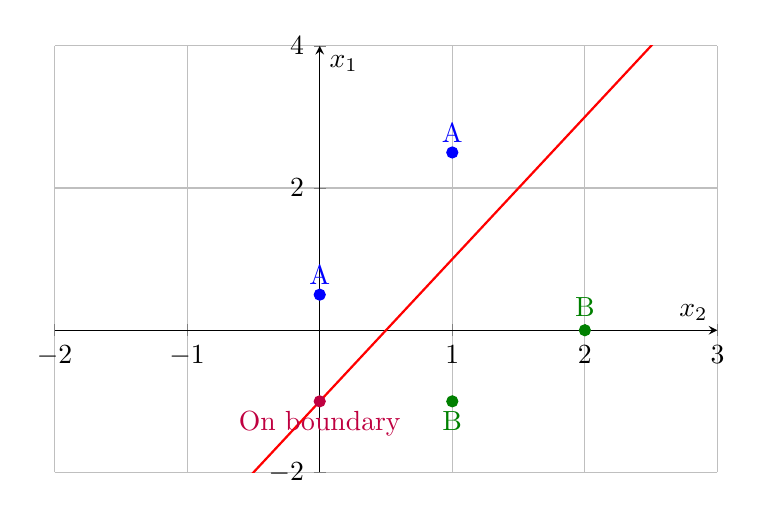
\begin{tikzpicture}
  \begin{axis}[
    axis lines=middle,
    xlabel={$x_2$}, ylabel={$x_1$},
    xmin=-2, xmax=3, ymin=-2, ymax=4,
    grid=major,
    width=10cm, height=7cm,
  ]

    % Decision boundary line: x_1 = 2x_2 - 1
    \addplot[domain=-2:3, samples=100, thick, red] {2*x -1};

    % Some sample points on different sides
    \addplot[mark=*,blue] coordinates {(0,0.5)};  % Check sign: 0.5 - 2*0 +1=1.5>0 => A
    \node[blue, anchor=south] at (axis cs:0,0.5) {A};
    
    \addplot[mark=*,blue] coordinates {(1,2.5)};  % Check: 2.5 - 2*1+1=2.5-2+1=1.5>0 => A
    \node[blue, anchor=south] at (axis cs:1,2.5) {A};
    
    \addplot[mark=*,purple] coordinates {(0,-1)};   % Check: -1 -2*(0)+1=0 => on boundary
    \node[purple, anchor=north] at (axis cs:0,-1) {On boundary};
    
    \addplot[mark=*,green!50!black] coordinates {(1,-1)}; % Check: -1 - 2*(1)+1=-1-2+1=-2<0 => B
    \node[green!50!black, anchor=north] at (axis cs:1,-1) {B};

    \addplot[mark=*,green!50!black] coordinates {(2,0)};   % Check:0 -2*(2)+1=0-4+1=-3<0 => B
    \node[green!50!black, anchor=north] at (axis cs:2,0.6) {B};

  \end{axis}
\end{tikzpicture}
\caption{\textit{A simple linear classifier in $\mathbb{R}^2$. The line $x_1 = 2x_2 - 1$ separates the plane into two classes. Points labeled A fall on one side, and points labeled B on the other.}}
\end{figure}

\noindent Here, the concept of a hyperplane from calculus—a linear construct that approximates behavior locally—appears in a machine learning context as a global decision boundary. Although the goal is different (classifying points rather than approximating a function at a point), the mathematical form is similar: a linear equation representing a flat boundary in space. This exemplifies how linear mathematical objects like lines, planes, and hyperplanes serve as foundational building blocks across various domains, from analyzing rates of change in calculus to making decisions in machine learning.


\subsection*{Linear Approximations: The Bridge Between Theory and Practice} \index{Linear Approximation}

\noindent Just as we used the tangent line in one dimension to approximate function values near a point, the tangent plane in two dimensions provides a linear approximation to \( f(x,y) \) near \((a,b)\). This approximation is extremely useful in many contexts:
\begin{itemize}
    \item \textbf{Estimating Values:} If we know \( f(a,b) \) and the partial derivatives at \((a,b)\), we can estimate \( f(x,y) \) for \((x,y)\) close to \((a,b)\) without computing \( f \) directly.
    \item \textbf{Differentials:} We define differentials \( dx \) and \( dy \) as small increments in \( x \) and \( y \). Then the differential \( df \) at \((a,b)\) is:
    \[
    df = f_x(a,b) dx + f_y(a,b) dy.
    \]
    This quantity \( df \) represents the best linear prediction for the actual change \(\Delta f = f(a+dx,b+dy)-f(a,b)\) for small changes \( dx \) and \( dy \). It is the multivariable extension of \( dy = f'(a)dx \) from single-variable calculus.
    \item \textbf{Error Estimation:} Suppose you measure \( x \) and \( y \) with some small possible errors \(\Delta x\) and \(\Delta y\). Using the tangent plane approximation, you can estimate how these errors propagate into \( f \):
    \[
    \Delta f \approx f_x(a,b)\Delta x + f_y(a,b)\Delta y.
    \]
    This lets you gauge how sensitive the function is to changes in its input variables.
\end{itemize}

\noindent Thus, the progression is:
\[
\text{Single variable: Tangent line} \implies f(x) \approx f(a) + f'(a)(x-a).
\]
\[
\text{Two variables: Tangent plane} \implies f(x,y) \approx f(a,b) + f_x(a,b)(x-a) + f_y(a,b)(y-b).
\]

\noindent This parallel structure shows that the concept of a linear approximation—so central in understanding functions in one dimension—scales naturally to higher dimensions, giving us a powerful geometric and analytic tool to approximate and understand the behavior of multivariable functions near any given point.

\subsubsection*{Beyond the Linear Approximation:} 

In some situations, the linear approximation may not provide sufficient information. For instance, if \(\nabla f(a,b) = \mathbf{0}\) (all first-order partial derivatives vanish), then the tangent plane is flat and does not reveal how \( f \) changes for small deviations from \((a,b)\). In such cases, we look to higher-order approximations, much like we use second- or third-order Taylor polynomials in single-variable calculus. \\

\noindent In two variables, a second-order approximation (also known as the quadratic approximation) includes second partial derivatives:
\[
\begin{split}
f(x,y) &\approx f(a,b) + f_x(a,b)(x-a) + f_y(a,b)(y-b) \\
&\quad + \tfrac{1}{2}\bigl[f_{xx}(a,b)(x-a)^2 + 2f_{xy}(a,b)(x-a)(y-b) + f_{yy}(a,b)(y-b)^2\bigr].
\end{split}
\]

\noindent These higher-order terms capture curvature and more subtle changes in the function. They can distinguish between extrema and provide more accurate estimates when larger changes in \( x \) and \( y \) occur. \\

\noindent While the linear approximation (tangent plane) is often the first and most accessible tool, knowing that higher-order expansions exist broadens your ability to model and understand complex phenomena. Whether adjusting manufacturing parameters, forecasting economic indicators, or analyzing stability in physical systems, having the option to include second-order (or higher) terms allows for richer, more nuanced approximations.

\exampleline
\begin{example}
A drone mapping a field captures the elevation of the terrain using the function:
\[
f(x,y) = 1000 - (x-25)^2 - \tfrac{1}{2}(y-50)^2,
\]
where \(x\) and \(y\) are coordinates in meters, and \(f(x,y)\) gives the elevation in meters. At the reference point \((25,50)\), the elevation is \(f(25,50) = 1000\) meters. Suppose the drone slightly shifts its measurement to \((26,48)\).

\begin{enumerate}
    \item Use a first-order (linear) approximation at \((25,50)\) to estimate the elevation at \((26,48)\).
    \item Compute the actual elevation at \((26,48)\) and discuss why the linear approximation fails.
    \item Suggest and compute a second-order approximation to improve the estimate.
\end{enumerate}

\begin{solution}
\begin{enumerate}
    \item \textbf{First-Order Approximation:} \index{First-Order Approximation}
    
    The first-order approximation uses the tangent plane to estimate elevation. The general formula for the first-order (linear) approximation of a function \( f(x,y) \) at a reference point \( (a,b) \) is:
    \[
    f(x,y) \approx f(a,b) + f_x(a,b)(x - a) + f_y(a,b)(y - b)
    \]
    For the given function:
    \[
    f(x,y) = 1000 - (x-25)^2 - \tfrac{1}{2}(y-50)^2,
    \]
    the partial derivatives are:
    \[
    f_x(x,y) = -2(x-25), \quad f_y(x,y) = -(y-50).
    \]
    At the reference point \((25,50)\):
    \[
    f_x(25,50) = -2(25-25) = 0, \quad f_y(25,50) = -(50-50) = 0.
    \]
    Substituting these values into the first-order approximation formula:
    \[
    f(x,y) \approx f(25,50) + 0 \cdot (x - 25) + 0 \cdot (y - 50) = 1000.
    \]
    Since both partial derivatives are zero at \((25,50)\), the linear approximation is a constant:
    \[
    f(x,y) \approx 1000.
    \]
    Using this approximation, the predicted elevation at \((26,48)\) is:
    \[
    f(26,48) \approx 1000.
    \]
    
    \item \textbf{Actual Elevation:}
    
    Compute the exact elevation at \((26,48)\):
    \[
    f(26,48) = 1000 - (26-25)^2 - \tfrac{1}{2}(48-50)^2.
    \]
    Simplify step by step:
    \[
    f(26,48) = 1000 - 1 - \tfrac{1}{2}(4) = 1000 - 1 - 2 = 997.
    \]
    The actual elevation is \(997\) meters, but the linear approximation predicted \(1000\). The error occurs because the tangent plane is flat at \((25,50)\), failing to capture the curvature of the terrain. In fact, our scheme will predict everything to be flat since $f(25,50)$ is constant. If we are very far up the terrain when this approximation is made, it'll only get much worse the farther out we go.
    
    \item \textbf{Second-Order Approximation:}  \index{Second-Order Approximation}
    
    To account for curvature, we use a second-order Taylor approximation:
\[
\begin{split}
f(x,y) &\approx f(a,b) + f_x(a,b)(x-a) + f_y(a,b)(y-b) \\
&\quad + \tfrac{1}{2}\bigl[f_{xx}(a,b)(x-a)^2 + 2f_{xy}(a,b)(x-a)(y-b) + f_{yy}(a,b)(y-b)^2\bigr].
\end{split}
\]
Compute the second derivatives:
    \[
    f_{xx}(x,y) = -2, \quad f_{yy}(x,y) = -1, \quad f_{xy}(x,y) = 0.
    \]
    The second-order approximation is:
\[
\begin{split}
f(x,y) &\approx f(25,50) + \tfrac{1}{2}\bigl[f_{xx}(25,50)(x-25)^2 \\
&\quad + 2f_{xy}(25,50)(x-25)(y-50) \\
&\quad + f_{yy}(25,50)(y-50)^2\bigr].
\end{split}
\]

    Substituting the derivatives and evaluating at \((26,48)\):
    \[
    f(26,48) \approx 1000 + \tfrac{1}{2}\bigl[-2(1)^2 + 0 + (-1)(-2)^2\bigr].
    \]
    Simplify:
    \[
    f(26,48) \approx 1000 + \tfrac{1}{2}(-2 - 4) = 1000 - \tfrac{6}{2} = 1000 - 3 = 997.
    \]
    The second-order approximation recovers the actual value, showing that considering curvature is crucial when first-order terms vanish.
    
    \item \textbf{Conclusion:}
    
    For flat terrain at a critical point (where the gradient is zero), higher-order terms reveal how the elevation changes. The second-order approximation includes curvature information, making it essential for accurate predictions in such cases.
\end{enumerate}
\end{solution}
\end{example}
\exampleline




\newpage

\lecture{Extrema and Critical Points}

\noindent One of the central themes in calculus is understanding where a function attains its greatest or least values. In single-variable calculus, this investigation led us to examine critical points—points where the derivative vanishes—and to use second-derivative tests to classify the nature of these points. These critical points allowed us to identify local maxima, local minima, and to note where the function’s concavity changes (potentially at points of inflection). Such insights gave us a clear understanding of the ``shape" of a curve along a one-dimensional axis. Because plotting is more challenging in higher dimensions, any analogy or simpler scenario that helps us visualize these concepts is useful. Not only this, but for optimization we will find extrema to be a cornerstone, just as we saw in single variable calculus. \\

\noindent As we move to functions of several variables, the problem becomes richer and more complex. Instead of analyzing a single input-output relationship along a line, we now consider surfaces (or even higher-dimensional objects) defined by multiple input variables. The notion of ``increasing" or ``decreasing" can no longer be grasped by simply looking to the left or right. We must consider changes in all possible directions around a point (often referred to as examining a \textit{neighborhood}). Consequently, the identification and classification of maxima, minima, and other special points (such as saddle points) demand more sophisticated tools and a broader conceptual framework. 

\subsection*{Single-Variable Concepts and Their Limitations} \index{Critical Points}

\noindent Let’s start by recalling what we know from single-variable calculus. For a differentiable function \( f: \mathbb{R} \to \mathbb{R} \):
\begin{itemize}
    \item A \textbf{critical point} \( x = a \) is where \( f'(a) = 0 \) or \( f'(a) \) does not exist.
    \item At such points, the function might have a local maximum or minimum, or it might simply change its curvature, suggesting a point of inflection (though not necessarily an extremum).
    \item To distinguish maxima and minima from other behaviors, we use the \textbf{second derivative test}:
    \begin{itemize}
        \item[$\circ$] If \( f''(a) > 0 \), the function is concave up at \( a \), typically indicating a local minimum.
        \item[$\circ$] If \( f''(a) < 0 \), the function is concave down at \( a \), typically indicating a local maximum.
        \item[$\circ$] If \( f''(a) = 0 \), the test is inconclusive and the behavior around \( a \) requires further investigation.
    \end{itemize}
    \item A \textbf{point of inflection} occurs at \( x = a \) if the function changes concavity (from concave up to concave down, or vice versa) at that point. To identify such points:
    \begin{itemize}
        \item[$\circ$] Compute \( f''(x) \) and find where \( f''(x) = 0 \) or \( f''(x) \) does not exist.
        \item[$\circ$] Check the sign of \( f''(x) \) on either side of \( x = a \). A change in sign confirms a point of inflection.
    \end{itemize}
\end{itemize}


%---------------------------
% A Basic Figure Demonstrating Extrema in One Variable
%---------------------------
\begin{figure}[H]
\centering
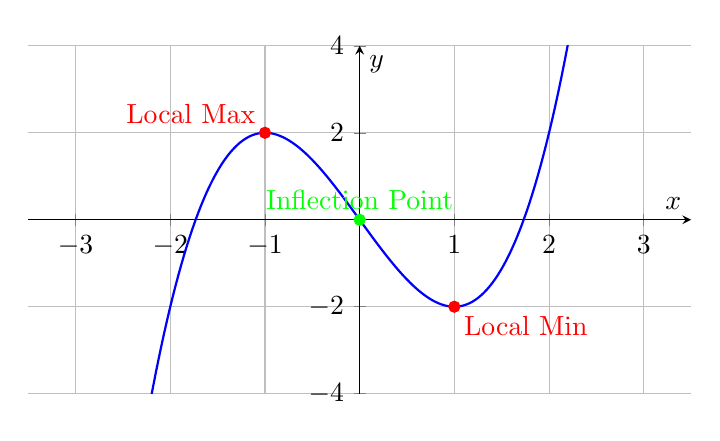
\begin{tikzpicture}
  \begin{axis}[
    axis lines=middle,
    xlabel={$x$}, ylabel={$y$},
    xmin=-3.5, xmax=3.5,
    ymin=-4, ymax=4,
    grid=major,
    width=10cm, height=6cm,
    domain=-3:3,
    samples=200,
  ]
    % Example function: f(x) = x^3 - 3x
    % f'(x)=3x^2 - 3; f''(x)=6x
    % Critical points: f'(x)=0 => 3x^2-3=0 => x^2=1 => x=±1.
    % At x=1, f''(1)=6(1)=6>0 -> local min at (1,1^3-3*1=1-3=-2)
    % At x=-1, f''(-1)=6(-1)=-6<0 -> local max at (-1, -(-3)=2)
    % Inflection point: f''(x)=0 => x=0, y=0^3-3*0=0
    \addplot[blue, thick] {x^3 - 3*x};

    % Mark critical points
    \addplot[mark=*, only marks, color=red] coordinates {(-1,2)}; % local max
    \addplot[mark=*, only marks, color=red] coordinates {(1,-2)}; % local min
    \addplot[mark=*, only marks, color=green] coordinates {(0,0)}; % inflection

    % Labels for points
    \node[above left, red] at (axis cs:-1,2) {Local Max};
    \node[below right, red] at (axis cs:1,-2) {Local Min};
    \node[above, green] at (axis cs:0,0) {Inflection Point};

  \end{axis}
\end{tikzpicture}
\caption{\textit{A single-variable function \(f(x)=x^3-3x\) illustrating a local maximum, local minimum, and an inflection point. The critical points at \(x=-1\) and \(x=1\) correspond to a local maximum and local minimum, respectively, while \(x=0\) is a point of inflection where the curvature changes.}}
\end{figure}

\noindent In the figure above, we see an example function \( f(x)=x^3 - 3x \) that has:
\begin{itemize}
    \item A local maximum at \( x=-1 \).
    \item A local minimum at \( x=1 \).
    \item An inflection point at \( x=0 \), where the graph changes from concave down to concave up.
\end{itemize}


\noindent These principles form the basis of understanding how functions behave near critical points in one dimension. However, when we move to multiple variables, these ideas must be generalized. Instead of a single derivative, we have partial derivatives. Instead of a single second derivative, we have a matrix of second-order partial derivatives (the Hessian). Instead of a single direction to check for concavity changes, we must consider changes in every direction. Because Linear Algebra is not a prerequisite to Multivariate Calculus, we will take this slow, don't worry. The complexity and richness of these scenarios make the transition from one-dimensional to multivariable calculus both challenging and rewarding. \\


\noindent The framework above allowed us to solve a variety of one-dimensional optimization problems. However, this approach heavily relies on the fact that there's only one independent variable. Extending these ideas to multiple variables introduces several challenges:
\begin{itemize}
    \item \textbf{Directionality:} In one dimension, you look left and right. In multiple dimensions, you must consider infinitely many directions from a point.
    \item \textbf{Multidimensional Curvature:} Instead of a single second derivative, we have a whole matrix of second derivatives (the Hessian).
    \item \textbf{Types of Critical Points:} With more directions come new types of stationary behavior. In particular, \textit{saddle points} arise, which are not maxima or minima, but still have zero gradient.
\end{itemize}

\subsection*{Extrema in Several Variables} \index{Extrema in Several Variables}


\noindent Generalizing some of the concepts to higher dimensions comes naturally enough with the notational conventions we have established in previous lectures. Consider a function \( f: \mathbb{R}^n \to \mathbb{R} \). We say that \( \mathbf{a} \in \mathbb{R}^n \) is an \textbf{extremum} of \( f \) if \( f(\mathbf{a}) \) is a maximum or minimum value of \( f \) in some sense. As in one dimension, we distinguish between:
 \index{Local Extrema} \index{Local Minima} \index{Local Maxima}
\begin{itemize}
    \item \textbf{Local Maximum in \(\mathbb{R}^n\)}: \( f(\mathbf{a}) \) is greater than or equal to \( f(\mathbf{x}) \) for all points \(\mathbf{x}\) in some ``small neighborhood" around \(\mathbf{a}\).
    \item \textbf{Local Minimum in \(\mathbb{R}^n\)}: \( f(\mathbf{a}) \) is less than or equal to \( f(\mathbf{x}) \) for all points \(\mathbf{x}\) in a small neighborhood around \(\mathbf{a}\).
    \item \textbf{Global Maximum/Minimum}: The value at \(\mathbf{a}\) is the supreme representative—no points in the entire domain beat it (for a max) or undercut it (for a min).
\end{itemize}
\noindent Below we see a 3D plot displaying all these extrema. Because we choose a function on a region $R = [-5,5] \times [-5,5]$ that has no division, and thus no points in the plot that go off to $\pm \infty$, we are guaranteed global extrema due the closed and bounded nature of the conditions. We will learn about this as the Extreme Value Theorem for multivariate functions.

\begin{figure}[H]
\centering
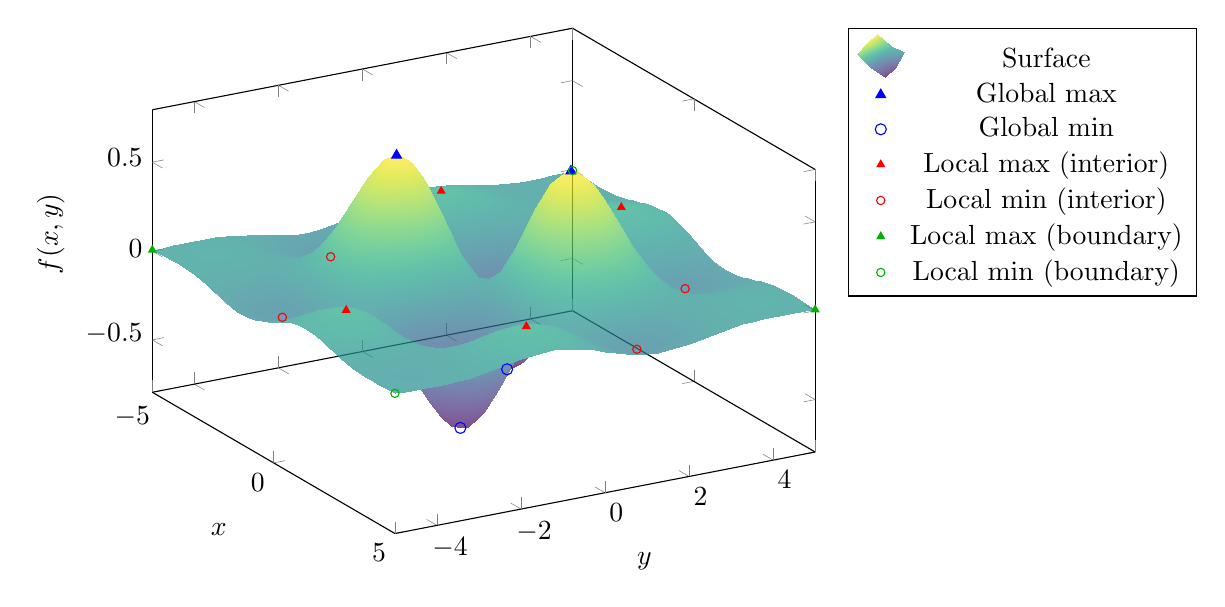
\begin{tikzpicture}
  \begin{axis}[
    view={60}{30},
    domain=-5:5, 
    domain y=-5:5,
    xlabel=$x$, ylabel=$y$, zlabel={$f(x,y)$},
    samples=41,
    width=10cm,
    height=8cm,
    legend style={at={(1.05,1)},anchor=north west}
  ]
    % Surface
    \addplot3[
      surf,
      shader=interp,
      opacity=0.7,
      colormap/viridis
    ] {sin(deg(x))*sin(deg(y))*exp(-0.1*(x^2+y^2))};
    \addlegendentry{Surface}

    % Global maxima (max=triangle)
    \addplot3[blue,mark=triangle*,only marks,mark size=2pt]
    coordinates {
      (-1.3154,-1.3154,0.6623)
      (1.3154,1.3154,0.6623)
    };
    \addlegendentry{Global max}

    % Global minima (min=circle)
    \addplot3[blue,mark=o,only marks,mark size=2pt]
    coordinates {
      (1.3154,-1.3154,-0.6623)
      (-1.3154,1.3154,-0.6623)
    };
    \addlegendentry{Global min}

    % Local maxima (interior) (max=triangle)
    \addplot3[red,mark=triangle*,only marks,mark size=1.5pt]
    coordinates {
      (1.3154,-4.0330,0.1245)
      (-4.0330,1.3154,0.1245)
      (4.0330,-1.3154,0.1245)
      (-1.3154,4.0330,0.1245)
    };
    \addlegendentry{Local max (interior)}

    % Local minima (interior) (min=circle)
    \addplot3[red,mark=o,only marks,mark size=1.5pt]
    coordinates {
      (4.0330,1.3154,-0.1245)
      (1.3154,4.0330,-0.1245)
      (-1.3154,-4.0330,-0.1245)
      (-4.0330,-1.3154,-0.1245)
    };
    \addlegendentry{Local min (interior)}

    % Local maxima (boundary) at (-5,-5) and (5,5) (max=triangle)
    \addplot3[green!70!black,mark=triangle*,only marks,mark size=1.5pt]
    coordinates {
      (-5,-5,0.006195)
      (5,5,0.006195)
    };
    \addlegendentry{Local max (boundary)}

    % Local minima (boundary) at (5,-5) and (-5,5) (min=circle)
    \addplot3[green!70!black,mark=o,only marks,mark size=1.5pt]
    coordinates {
      (5,-5,-0.006195)
      (-5,5,-0.006195)
    };
    \addlegendentry{Local min (boundary)}

  \end{axis}
\end{tikzpicture}
\caption{\textit{The surface plot of $f(x,y) = \sin(x)\sin(y)e^{-0.1(x^2 + y^2)}$ with annotated extrema. No laughing, please.}}
\label{fig:extrema_ex}
\end{figure}

\noindent However, unlike the single-variable case, ``small neighborhood” is not just an interval around a point. In \(\mathbb{R}^n\), you can approach a point from infinitely many directions. There can be ``flat” regions where the function doesn't change for a while, disconnected parts of the domain, and directions in which the function heads off to infinity (no global extrema exist). Thus, while the idea of local and global maxima and minima transfers directly, the complexity of higher dimensions makes the identification and classification of these points more subtle.

\subsubsection*{A Rigorous Approach}

Before we dive into the rigor, we need to define the concepts of \textbf{open sets}, \textbf{closed sets}, \textbf{balls}, and \textbf{compactness}. Understanding these definitions is crucial for formalizing our discussions on neighborhoods and extrema in multiple dimensions.

\begin{itemize}
    \item \textbf{Open Set}: \index{Open Sets} A set \( U \subset \mathbb{R}^n \) is called \textit{open} if, for every point \( \mathbf{a} \in U \), you can move a little bit in any direction from \( \mathbf{a} \) and still stay within \( U \). In other words, there are no ``edge" points included in \( U \). This is essentially the higher dimensional analog of an open interval $(a,b)$.
    
    \item \textbf{Closed Set}: \index{Closed Sets} A set \( C \subset \mathbb{R}^n \) is called \textit{closed} if it includes all its boundary points. This means that if you have a sequence of points within \( C \) that gets closer and closer to some point \( \mathbf{x} \), then \( \mathbf{x} \) is also included in \( C \). This is essentially the higher dimensional analog of a closed interval $[a,b]$.


%---------------------------------------
% Illustration of disjoint open set U and closed set C
%---------------------------------------
\begin{figure}[H]
\centering
\begin{tikzpicture}
  % Open Set U
  \begin{axis}[
    width=6cm, height=6cm,           % Smaller size
    axis lines=none,                 % Remove axes
    clip=false,                      % Allow plotting outside axis bounds
    xlabel style={font=\small}, ylabel style={font=\small},
    tick label style={font=\small},
    title={Open Set $U$},            % Title for open set
    title style={font=\small, at={(0.5,-0.1)}, anchor=north}, % Center title below plot
    ]
    % Dotted boundary
    \addplot[
      domain=0:360,
      samples=100,
      dashed,
      thick
    ] (
      {cos(x)},
      {sin(x)}
    );
  \end{axis}

  % Closed Set C
  \begin{axis}[
    at={(7cm,0)},                    % Place side by side with some separation
    width=6cm, height=6cm,           % Smaller size
    axis lines=none,                 % Remove axes
    clip=false,                      % Allow plotting outside axis bounds
    xlabel style={font=\small}, ylabel style={font=\small},
    tick label style={font=\small},
    title={Closed Set $C$},          % Title for closed set
    title style={font=\small, at={(0.5,-0.1)}, anchor=north}, % Center title below plot
    ]
    % Solid boundary
    \addplot[
      domain=0:360,
      samples=100,
      thick
    ] (
      {cos(x)},
      {sin(x)}
    );
  \end{axis}
\end{tikzpicture}
\caption{\textit{Illustration of an open set $U$ with a dotted boundary and a closed set $C$ with a solid boundary.}}
\end{figure}

    
    \item \textbf{Open Ball}: An open ball in \( \mathbb{R}^n \) centered at \( \mathbf{a} \) with radius \( \epsilon \) is the set of all points \( \mathbf{x} \) such that the distance between \( \mathbf{x} \) and \( \mathbf{a} \) is less than \( \epsilon \). It is defined as:
    \[
    B_{\epsilon}(\mathbf{a}) = \left\{ \mathbf{x} \in \mathbb{R}^n \mid \|\mathbf{x} - \mathbf{a}\| < \epsilon \right\}.
    \]
    
    \item \textbf{Compact Set}: \index{Compact Sets} A set \( D \subset \mathbb{R}^n \) is called \textit{compact} if it is both closed and bounded. This means that \( D \) contains all its boundary points and fits within some finite region of space.
\end{itemize}

\noindent To handle these complexities, we need a more precise definition of what it means to be ``close" to a point in multiple dimensions. In one dimension, being close to \( a \) meant \( |x - a| < \epsilon \) for some \(\epsilon > 0\). In \(\mathbb{R}^n\), we generalize this by using open balls defined by a norm. A standard choice is the Euclidean norm \( \|\cdot\| \), which represents the usual distance between vectors. Thus, we define:
\[
B_{\epsilon}(\mathbf{a}) = \left\{ \mathbf{x} \in \mathbb{R}^n \mid \|\mathbf{x} - \mathbf{a}\| < \epsilon \right\}.
\]
This \( B_{\epsilon}(\mathbf{a}) \) is an \textit{open ball} of radius \(\epsilon\) centered at \( \mathbf{a} \). It serves as the higher-dimensional analogue of a small interval around a point.
\\

\noindent With this notation, we can restate the definitions more rigorously:
\begin{itemize}
    \item \textbf{Local Maximum:} A point \(\mathbf{a}\) is a local maximum of \( f \) if there exists \(\epsilon >0\) such that for all \(\mathbf{x} \in B_{\epsilon}(\mathbf{a})\),
    \[
    f(\mathbf{x}) \leq f(\mathbf{a}).
    \]
    Here, ``all \(\mathbf{x}\) in \( B_{\epsilon}(\mathbf{a})\)" means we are checking every direction and every point sufficiently close to \(\mathbf{a}\).

    \item \textbf{Local Minimum:} A point \(\mathbf{a}\) is a local minimum of \( f \) if there exists \(\epsilon > 0\) such that for all \(\mathbf{x} \in B_{\epsilon}(\mathbf{a})\),
    \[
    f(\mathbf{x}) \geq f(\mathbf{a}).
    \]

    \item \textbf{Global Maximum/Minimum:} These are defined similarly to the single-variable case, but we consider the entire domain. A point \(\mathbf{a}\) is a global maximum if
    \[
    f(\mathbf{x}) \leq f(\mathbf{a}) \text{ for all } \mathbf{x} \in \text{dom}(f).
    \]
    And similarly for a global minimum.
\end{itemize}

\noindent Using these $\epsilon$-ball/neighborhood definitions makes our concepts more robust. For instance, the notion of local extremum now doesn’t depend on the shape of the domain or the peculiarities of how we approach the point \(\mathbf{a}\). Instead, it inherently encodes the idea of “closeness" and “no other nearby points exceeding (or undercutting) the value at \(\mathbf{a}\)." \\

\noindent This refined perspective also ties in with deeper results from real analysis. For example, if \( f \) is continuous on a compact set \( D \subset \mathbb{R}^n \), the Extreme Value Theorem guarantees the existence of global maxima and minima. However, if the domain is not compact, or if \( f \) is not nicely behaved, we may fail to find global extrema. The function may “escape” to infinity in some direction, preventing a global maximum or minimum from forming. 


\subsubsection*{Local vs. Global Extrema} \index{Global Extrema} \index{Global Minima} \index{Global Maxima}

\noindent The \textit{Extreme Value Theorem} from single-variable calculus ensures that if a continuous function is defined on a closed interval, it attains global maxima and minima. In higher dimensions, there is a corresponding result: if \( f \) is continuous on a \textit{compact set} \( D \subset \mathbb{R}^n \) (i.e., \( D \) is closed and bounded), then \( f \) attains both a global maximum and a global minimum on \( D \). However, if the domain is not compact, the situation is more complex:
\begin{itemize}
    \item If the domain is not bounded, \( f \) may ``escape" to infinity, never settling on a highest or lowest value.
    \item If the domain is open or lacks a boundary, local conditions might not guarantee global extremality.
\end{itemize}

\noindent Understanding these nuances is crucial in applications. For example, in optimization problems with constraints, ensuring the constraint set is compact (often via bounding conditions) can help guarantee that a solution (a global extremum) exists. \\

\noindent Consider a two-dimensional function \( f(x,y) \) that forms a surface in \(\mathbb{R}^3\). A local maximum appears like a peak in some \(\epsilon\)-ball around \((a,b)\); a local minimum looks like a valley. If the surface keeps rising as \( x^2+y^2 \to \infty \) (like a giant unbounded mountain), no global maxima exist because we can always find higher points. Similarly, if it keeps going downwards without bound, no global minima exist.



%---------------------------------------
% Insert a figure illustrating a local maximum on a surface with an epsilon ball around the global max
%---------------------------------------
\begin{figure}[H]
\centering
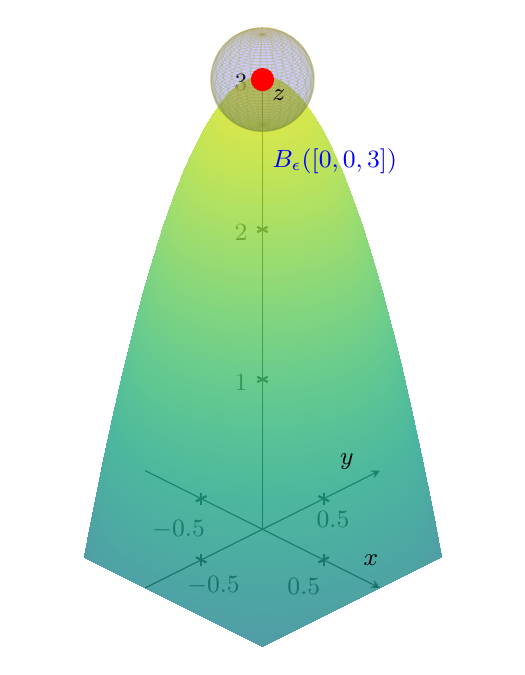
\begin{tikzpicture}
  \pgfmathsetmacro{\plotwidth}{13}  % Adjustable width in cm
  \pgfmathsetmacro{\plotheight}{13} % Adjustable height in cm
  \begin{axis}[
    view={45}{30},                     % Adjust the viewing angle
    xlabel={$x$}, ylabel={$y$}, zlabel={$z$},
    axis lines=middle,                 % Only draw the axes through the middle
    domain=-1:1, y domain=-1:1,
    samples=50, samples y=50,          % Increase sample density for better resolution
    width=\plotwidth cm, height=\plotheight cm, % Use adjustable dimensions
    colormap/viridis,
    zmin=0, zmax=3,
    clip=true,                          % Ensure plot elements are clipped to the axis area
    enlargelimits=false,                % Prevent automatic enlargement of plot limits
    tick style={thick, black},          % Thicker ticks for better visibility
    tick label style={font=\small},     % Consistent font size for tick labels
    xlabel style={font=\small},         % Consistent font size for labels
    ylabel style={font=\small},
    zlabel style={font=\small},
    axis equal image,                   % Ensure equal scaling for all axes
    ]
      % Plot the surface with a local maximum at (0,0,3)
      \addplot3[
        surf,
        opacity=0.8,
        shader=interp,                    % Smooth shading for better appearance
      ] 
      {3 - 3*(x^2 + y^2)};
      
      % Mark the top point (0,0,3) with a red dot
      \addplot3[
        only marks,
        mark=*,
        color=red,
        mark size=4pt,                    % Increase marker size for visibility
      ] 
      coordinates {(0,0,3)};
      
      % Define epsilon
      \pgfmathsetmacro{\eps}{0.3}
      
      % Add an epsilon-ball (sphere) around the global maximum (0,0,3)
      \addplot3[
        surf,
        opacity=0.1,                      % Increased transparency
        color=blue,
        samples=30,                       % Increase sphere resolution
        domain=0:360,
        y domain=0:180,
      ]
      (
        {\eps * sin(y) * cos(x)},
        {\eps * sin(y) * sin(x)},
        {3 + \eps * cos(y)}
      );
      
      % Add a label for the epsilon ball
      \node at (axis cs:\eps,-.3,2.7) [anchor=west, color=blue, font=\small] {$B_\epsilon([0,0,3])$};
  \end{axis}
\end{tikzpicture}
\caption{\textit{A surface with a global maximum at the origin. The red dot marks the global maximum at $(0, 0, 3)$. The blue semi-transparent sphere represents a $B_\epsilon([0,0,3])$, illustrating a neighborhood within which no other points have a higher value. As we move away from the origin, the surface descends, ensuring that the global maximum is maintained within the $B_\epsilon([0,0,3])$.}}
\end{figure}





\noindent In the figure above, we see a simple example: \( f(x,y)=3 - 3(x^2+y^2) \) has a local maximum at \((0,0)\) where \( f(0,0)=3 \). In fact, this is also a global maximum since the function decreases as we move away from \((0,0)\), approaching negative infinity without bound. If we had a function that only rose at the origin and flattened out or grew in other directions, we might not have any global maxima or minima, just local ones. 



\exampleline
\begin{example}
Consider the Extreme Value Theorem (EVT) \index{Extreme Value Theorem} in the context of multivariable calculus, which states that if a function \( f: \mathbb{R}^n \to \mathbb{R} \) is continuous on a \textit{compact} set \( D \) (i.e., \( D \) is closed and bounded), then \( f \) attains both a global maximum and a global minimum on \( D \).

\begin{enumerate}
    \item Provide an example of a continuous function defined on an \textbf{unbounded} domain in \( \mathbb{R}^2 \) that does \textbf{not} attain a global maximum or a global minimum. Explain why this example illustrates the necessity of the boundedness condition in EVT.
    
    \item Provide an example of a continuous function defined on an \textbf{open} (not closed) and \textbf{bounded} domain in \( \mathbb{R}^2 \) that does \textbf{not} attain a global maximum or a global minimum. Explain why this example illustrates the necessity of the closedness condition in EVT.
\end{enumerate}


\begin{solution}
\begin{enumerate}
\item Consider the function \( f: \mathbb{R}^2 \to \mathbb{R} \) defined by
\[
f(x, y) = x.
\]

\begin{itemize}
    \item \textbf{Domain Unbounded:} The domain \( \mathbb{R}^2 \) is unbounded, meaning it extends infinitely in all directions.
    
    \item \textbf{Behavior of \( f(x, y) \):}
    \begin{itemize}
        \item As \( x \to \infty \), \( f(x, y) \to \infty \).
        \item As \( x \to -\infty \), \( f(x, y) \to -\infty \).
    \end{itemize}
    
    \item \textbf{Global Extrema:} 
    \begin{itemize}
        \item Global Maximum: \( f \) does not attain a global maximum because for any value \( M \), there exists \( (x, y) \in \mathbb{R}^2 \) with \( x > M \).
        \item Global Minimum: Similarly, \( f \) does not attain a global minimum because for any value \( m \), there exists \( (x, y) \in \mathbb{R}^2 \) with \( x < m \).
    \end{itemize}
    
    \item \textbf{Conclusion:} This example demonstrates that when the domain is unbounded, a continuous function may fail to attain global extrema. This highlights the necessity of the boundedness condition in the Extreme Value Theorem to ensure the existence of both a global maximum and a global minimum.
\end{itemize}

\item Consider the function \( g: D \to \mathbb{R} \) defined by
\[
g(x, y) = \frac{1}{1 - x^2 - y^2},
\]
where the domain \( D = \{ (x, y) \in \mathbb{R}^2 \mid x^2 + y^2 < 1 \} \) is the open unit disk.

\begin{itemize}
    \item \textbf{Domain Not Closed:} The domain \( D \) is open because it does not include the boundary \( x^2 + y^2 = 1 \). While \( D \) is bounded, it lacks closure.
    
    \item \textbf{Behavior of \( g(x, y) \):}
    \begin{itemize}
        \item As \( (x, y) \) approaches the boundary of \( D \) (i.e., as \( x^2 + y^2 \to 1 \)), the denominator \( 1 - x^2 - y^2 \to 0 \), causing \( g(x, y) \to \infty \).
        \item Within \( D \), \( g(x, y) \) is always positive and increases without bound near the boundary.
    \end{itemize}
    
    \item \textbf{Global Extrema:} 
    \begin{itemize}
        \item Global Maximum: \( g \) does not attain a global maximum because for any large value \( M \), there exists \( (x, y) \in D \) sufficiently close to the boundary such that \( g(x, y) > M \).
        \item Global Minimum:
        \begin{itemize}
            \item \( g \) does attain a global minimum at the center \( (0, 0) \), where \( g(0, 0) = 1 \).
            \end{itemize}
    \end{itemize}
    
    \item \textbf{Conclusion:} Although \( g \) attains a global minimum, it fails to attain a global maximum because the domain \( D \) is not closed. This example illustrates that the closedness condition is necessary in the Extreme Value Theorem to ensure that all global extrema are attained.
\end{itemize}
\end{enumerate}

\end{solution}
\end{example}


\exampleline

\subsection*{First Derivative Test for Extrema: Critical Points in Multiple Dimensions} \index{First Derivative Test}

\noindent In single-variable calculus, the process of finding candidates for local extrema is straightforward: we compute \( f'(x) \), set it equal to zero, and solve for \( x \). Points where \( f'(x)=0 \) or \( f'(x) \) is undefined are the \textbf{critical points}, and each such point is examined to determine whether it corresponds to a local maximum, minimum, or neither. This procedure generalizes naturally to functions of several variables, but with an additional layer of complexity. \\

\noindent For a function \( f: \mathbb{R}^n \to \mathbb{R} \), the analogue to the single-variable derivative is the \textbf{gradient} vector:
\[
\nabla f(\mathbf{x}) = \left\langle \frac{\partial f}{\partial x_1}(\mathbf{x}), \frac{\partial f}{\partial x_2}(\mathbf{x}), \ldots, \frac{\partial f}{\partial x_n}(\mathbf{x}) \right\rangle.
\]
The gradient encodes the rate of change of \( f \) in each coordinate direction. Setting the gradient to zero:
\[
\nabla f(\mathbf{a}) = \mathbf{0}
\]
defines the \textbf{critical points} or \textbf{stationary points} of \( f \). At any such point \(\mathbf{a}\), the function \( f \) has no instantaneous tendency to increase or decrease in any of the standard coordinate directions. \\

To find critical points in practice, one must:
\begin{enumerate}
    \item Compute the partial derivatives \(\frac{\partial f}{\partial x_i}\) for each \( i = 1,2,\ldots,n \).
    \item Solve the system of equations:
    \[
    \frac{\partial f}{\partial x_1}(\mathbf{x})=0, \quad \frac{\partial f}{\partial x_2}(\mathbf{x})=0, \quad \ldots, \quad \frac{\partial f}{\partial x_n}(\mathbf{x})=0.
    \]
    Finding solutions may be straightforward for simple functions or can become highly nontrivial for more complicated ones, often requiring numerical methods or careful algebraic manipulation.

    \item Identify all points \(\mathbf{a}\) that satisfy these equations. Each such \(\mathbf{a}\) is a potential extremum, but additional steps are necessary to classify its nature.
\end{enumerate}

\noindent Having \(\nabla f(\mathbf{a}) = \mathbf{0}\) is a necessary condition for \(\mathbf{a}\) to be a local maximum or minimum, but this condition alone does not guarantee the existence of an extremum at \(\mathbf{a}\). Consider the single-variable analogy: if \( f'(a)=0 \), \( a \) might be a max, min, or even a point of inflection. In multiple dimensions, the situation is more nuanced:
\begin{itemize}
    \item A zero gradient could indicate a local maximum if the function “peaks" at that point.
    \item It could indicate a local minimum if the function “valleys" at that point.
    \item It could also indicate a \textit{saddle point}, where the function curves up in some directions and down in others, making the point neither a max nor a min. 
\end{itemize}

\noindent The gradient test (setting \(\nabla f(\mathbf{a})=0\)) is like a first filter. It narrows the set of candidate points that could be extrema, but it does not complete the classification. To fully determine the nature of each critical point, we must invoke second-order information, typically via the Hessian matrix, and apply a second derivative test in several variables. Only after analyzing the Hessian (or, more precisely, the definiteness of the Hessian matrix at \(\mathbf{a}\)) can we decide whether \(\mathbf{a}\) is a maximum, a minimum, or a saddle point. \\

\noindent Hence, the first derivative test in multiple dimensions leads us to identify critical points by solving a system of equations \(\nabla f(\mathbf{a})=\mathbf{0}\). While this can be challenging, it is a necessary step towards understanding the structure of the function’s graph, the locations of its extrema, and the detailed shape of its level surfaces. \\

\noindent As \( n \) grows, the complexity of setting all partial derivatives to zero increases significantly. In practice, for higher dimensions or more complicated functions, one often relies on numerical methods, optimization algorithms (like gradient descent), or specialized analytic techniques to locate critical points. The first derivative test is fundamental but can be quite involved in real-world scenarios. Let's take an example.


\exampleline
\begin{example} Determine the critical points of the following functions using the First Derivative Test.
    
    \begin{enumerate}
        \item \( f(x,y) = x^3 - 3xy^2 \)
        \item \( h(x,y,z) = x^2 + y^2 + z^2 - 4x - 6y - 8z \)
        \item \( g(x,y) = e^{x} + e^{y} + xy \)
    \end{enumerate}
    
    \begin{solution}
    \begin{enumerate}
        \item \textbf{Function \( f(x,y) = x^3 - 3xy^2 \)}
        
        \begin{enumerate}
            \item \textbf{Compute the Partial Derivatives:}
            \[
            f_x = \frac{\partial f}{\partial x} = 3x^2 - 3y^2
            \]
            \[
            f_y = \frac{\partial f}{\partial y} = -6xy
            \]
            
            \item \textbf{Set the Gradient Equal to Zero:}
            \[
            \nabla f = \langle 3x^2 - 3y^2, -6xy \rangle = \mathbf{0}
            \]
            This leads to the system:
            \[
            3x^2 - 3y^2 = 0 \quad \text{and} \quad -6xy = 0
            \]
            
            \item \textbf{Solve for Critical Points:}
            \[
            3x^2 - 3y^2 = 0 \implies x^2 = y^2
            \]
            \[
            -6xy = 0 \implies x = 0 \quad \text{or} \quad y = 0
            \]
            
            \begin{itemize}
                \item \textbf{Case 1:} \( x = 0 \)
                \[
                x^2 = y^2 \implies 0 = y^2 \implies y = 0
                \]
                Critical point: \( (0, 0) \)
                
                \item \textbf{Case 2:} \( y = 0 \)
                \[
                x^2 = 0 \implies x = 0
                \]
                Critical point: \( (0, 0) \)
            \end{itemize}
            
            Thus, the only critical point is \( (0, 0) \).
        \end{enumerate}
        
        \item \textbf{Function \( h(x,y,z) = x^2 + y^2 + z^2 - 4x - 6y - 8z \)}
        
        \begin{enumerate}
            \item \textbf{Compute the Partial Derivatives:}
            \[
            h_x = \frac{\partial h}{\partial x} = 2x - 4
            \]
            \[
            h_y = \frac{\partial h}{\partial y} = 2y - 6
            \]
            \[
            h_z = \frac{\partial h}{\partial z} = 2z - 8
            \]
            
            \item \textbf{Set the Gradient Equal to Zero:}
            \[
            \nabla h = \langle 2x - 4, 2y - 6, 2z - 8 \rangle = \mathbf{0}
            \]
            This leads to the system:
            \[
            2x - 4 = 0 \quad \Rightarrow \quad x = 2
            \]
            \[
            2y - 6 = 0 \quad \Rightarrow \quad y = 3
            \]
            \[
            2z - 8 = 0 \quad \Rightarrow \quad z = 4
            \]
            
            Thus, the critical point is \( (2, 3, 4) \).
        \end{enumerate}
        
        \item \textbf{Function \( g(x,y) = e^{x} + e^{y} + xy \)}
        
        \begin{enumerate}
            \item \textbf{Compute the Partial Derivatives:}
            \[
            g_x = \frac{\partial g}{\partial x} = e^{x} + y
            \]
            \[
            g_y = \frac{\partial g}{\partial y} = e^{y} + x
            \]
            
            \item \textbf{Set the Gradient Equal to Zero:}
            \[
            \nabla g = \langle e^{x} + y, e^{y} + x \rangle = \mathbf{0}
            \]
            This leads to the system:
            \[
            e^{x} + y = 0 \quad \text{and} \quad e^{y} + x = 0
            \]
            
            \item \textbf{Solve for Critical Points:}
            
            From the first equation:
            \[
            y = -e^{x}
            \]
            Substitute into the second equation:
            \[
            e^{-e^{x}} + x = 0
            \]
            This transcendental equation does not have a closed-form solution, so we identify the critical point numerically using Wolfram Alpha or another online tool. The approximate solution is:
            \[
            x \approx -0.567143, \quad y \approx -0.567143
            \]
            Thus, the approximate critical point is \( \left( -0.567143, -0.567143 \right) \).
        \end{enumerate}
    \end{enumerate}
    \end{solution}
\end{example}
\exampleline


\subsection*{Second Derivative Tests for Functions of Two Variables} \index{Second Derivative Test}

\noindent After employing the first derivative test (i.e., finding points where the gradient \(\nabla f = \mathbf{0}\)) to identify critical points of a two-variable function \( f(x,y) \), the next step is to determine the nature of these critical points: are they local maxima, local minima, or something else? In single-variable calculus, this classification depended on the sign of the second derivative \( f''(a) \). In the two-variable setting, we must consider second partial derivatives and how they interact.

\subsubsection*{From Single to Multiple Variables: The Discriminant} \index{Discriminant}

\noindent Let \( f: \mathbb{R}^2 \to \mathbb{R} \) be a function with continuous second partial derivatives. Suppose \((a,b)\) is a critical point, i.e.,
\[
f_x(a,b)=0 \quad \text{and} \quad f_y(a,b)=0.
\]

\noindent To classify \((a,b)\), we consider the second partial derivatives at \((a,b)\):
\[
f_{xx}(a,b)=\frac{\partial^2 f}{\partial x^2}(a,b), \quad f_{yy}(a,b)=\frac{\partial^2 f}{\partial y^2}(a,b), \quad f_{xy}(a,b)=\frac{\partial^2 f}{\partial x \partial y}(a,b).
\]

\noindent We define the \textbf{discriminant} \( D \) as:
\[
D = f_{xx}(a,b)f_{yy}(a,b) - [f_{xy}(a,b)]^2.
\]

\noindent This discriminant \( D \) encapsulates how the function curves in different directions near the critical point. Notably, \( D \) is also the determinant of the Hessian matrix at \((a,b)\) in two dimensions. The Hessian matrix arises because of the fact in a multivariate setting, the second derivatives of variables have to go through all the combinations of derivatives of two variables which gets messy in higher dimensions. For now, in two dimensions, the Hessian matrix \index{Hessian Matrix} is:
\[
H(a,b) = \begin{bmatrix} f_{xx}(a,b) & f_{xy}(a,b) \\ f_{yx}(a,b) & f_{yy}(a,b) \end{bmatrix}.
\]
And thus, 
\[
D=\det(H(a,b))=f_{xx}(a,b)f_{yy}(a,b)-[f_{xy}(a,b)]^2.
\]
More on the Hessian, and some of these linear algebra terms to come later.

\subsubsection*{Local Extrema} \index{Local Extrema}

\noindent Using the discriminant \( D \) and the sign of \( f_{xx}(a,b) \), we have a test analogous to the single-variable scenario:
\begin{itemize}
    \item If \( D > 0 \) and \( f_{xx}(a,b) > 0 \), \((a,b)\) is a \textbf{local minimum}.
    \item If \( D > 0 \) and \( f_{xx}(a,b) < 0 \), \((a,b)\) is a \textbf{local maximum}.
    \item If \( D < 0 \), \((a,b)\) is neither a max nor a min (it may be a saddle point).
    \item If \( D = 0 \), the test is inconclusive, requiring further analysis.
\end{itemize}

\noindent This gives us a direct way to classify local maxima and minima for functions of two variables once we know their first and second derivatives at a critical point.

\exampleline
\begin{example} Determine the nature of the critical point of the function \( f(x,y) = 2x^2 + 3y^2 - 4x - 6y + 10 \) using the Second Derivative Test.
    
    \begin{solution}
        \begin{enumerate}
            \item \textbf{Find the Critical Point}:
            
            \begin{enumerate}
                \item Compute the First Partial Derivatives:
                \[
                f_x = \frac{\partial f}{\partial x} = 4x - 4
                \]
                \[
                f_y = \frac{\partial f}{\partial y} = 6y - 6
                \]
                
                \item \textbf{Set the Gradient Equal to Zero}:
                \[
                \nabla f = \langle 4x - 4, 6y - 6 \rangle = \mathbf{0}
                \]
                Solving the system:
                \[
                4x - 4 = 0 \quad \Rightarrow \quad x = 1
                \]
                \[
                6y - 6 = 0 \quad \Rightarrow \quad y = 1
                \]
                
                Thus, the critical point is \( (1, 1) \).
            \end{enumerate}
            
            \item \textbf{Classify the Critical Point Using the Second Derivative Test}:
            
            \begin{enumerate}
                \item Compute the Second Partial Derivatives:
                \[
                f_{xx} = \frac{\partial^2 f}{\partial x^2} = 4, f_{yy} = \frac{\partial^2 f}{\partial y^2} = 6,  f_{xy} = \frac{\partial^2 f}{\partial x \partial y} = 0
                \]
                
                \item Calculate the Discriminant \( D \):
                \[
                D = f_{xx}(1,1) \cdot f_{yy}(1,1) - [f_{xy}(1,1)]^2 = (4)(6) - (0)^2 = 24 > 0
                \]
                
                \item Apply the Classification Rules:
                \begin{itemize}
                    \item Since \( D > 0 \) and \( f_{xx}(1,1) = 4 > 0 \), \( (1, 1) \) is a \textbf{local minimum}. Let's draw a picture! We can mark the local min with a red dot:
                \end{itemize}
            \end{enumerate}
        \end{enumerate}

            \begin{center}
            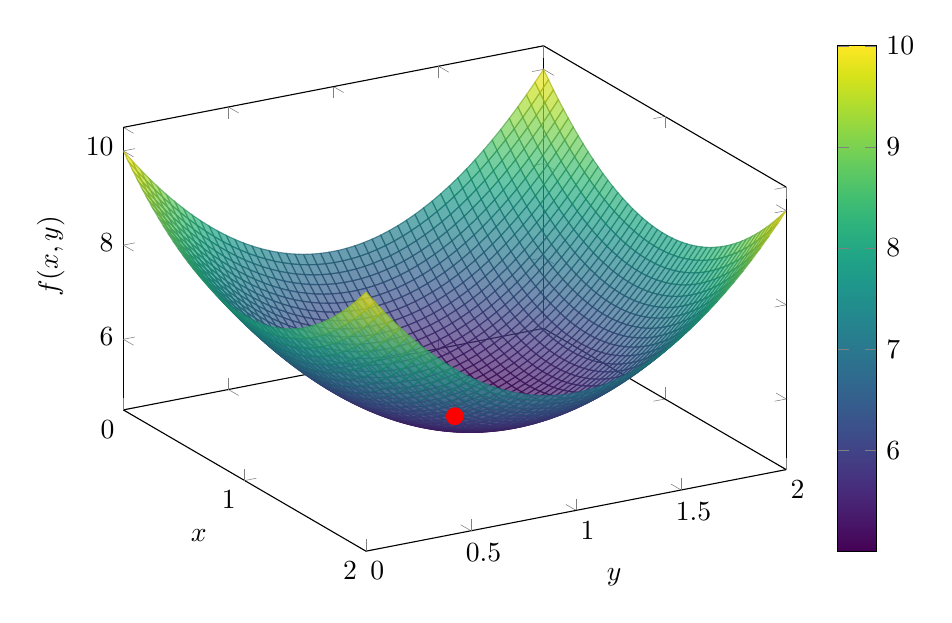
\begin{tikzpicture}
                \begin{axis}[
                    view={60}{30},
                    xlabel={$x$},
                    ylabel={$y$},
                    zlabel={$f(x,y)$},
                    domain=0:2,
                    y domain=0:2,
                    samples=50,
                    samples y=50,
                    colormap/viridis,
                    colorbar,
                    width=10cm,
                    height=8cm,
                ]
                \addplot3[
                    surf,
                    opacity=0.7,
                ]
                {2*x^2 + 3*y^2 - 4*x - 6*y + 10};
                
                % Plot the local minimum point
                \addplot3[
                    only marks,
                    mark=*,
                    mark size=3pt,
                    color=red,
                ]
                coordinates {(1,1,5)};
                
                % Annotate the local minimum
                \node at (axis cs:1,1,5) [anchor=north east, red] {};
                \end{axis}
            \end{tikzpicture}
            \end{center}
            


    \end{solution}
\end{example}
\exampleline


\subsubsection*{Global Extrema Considerations} \index{Global Extrema} 

\noindent While the second derivative test helps us determine local behavior near a critical point, identifying global maxima or minima is a separate question. In single-variable calculus, the Extreme Value Theorem guarantees that a continuous function defined on a closed, bounded interval attains a global maximum and minimum. Similarly, for functions of two variables, if \( f \) is continuous on a compact (closed and bounded) set in \(\mathbb{R}^2\), then \( f \) attains a global maximum and minimum on that set. \\

\noindent Finding global extrema typically involves:
\begin{enumerate}
    \item Identifying all critical points inside the domain.
    \item Checking the behavior on the boundary of the domain (since global extrema may occur there, not just at critical points).
    \item Comparing the values of \( f \) at these points to see which are the largest and smallest.
\end{enumerate}

\noindent If the domain is not compact—if it is unbounded or not closed—then \( f \) may fail to achieve global maxima or minima altogether. The function might ``escape" to infinity in some directions, or may never settle on a maximum value. Let's take a look at an example:


\exampleline
\begin{example} Determine the global maximum and minimum of the function \( f(x,y) = 2x^2 + 3y^2 - 4x - 6y + 10 \) on the closed and bounded region \( R \) defined by \( 0 \leq x \leq 3 \) and \( 0 \leq y \leq 3 \).
    
    \begin{solution}
        \begin{enumerate}
            \item \textbf{Identify Critical Points:}
            
            \begin{itemize}
                \item First Partial Derivatives:
                \[
                f_x = 4x - 4 \quad \text{and} \quad f_y = 6y - 6
                \]
                
                \item Setting the Gradient to Zero: 
                \[
                4x - 4 = 0 \quad \Rightarrow \quad x = 1
                \]
                \[
                6y - 6 = 0 \quad \Rightarrow \quad y = 1
                \]
                
                \item Critical Point:
                \[
                (1, 1)
                \]
            \end{itemize}
            
            \item \textbf{Classify the Critical Point Using the Second Derivative Test:}
            
            \begin{itemize}
                \item Second Partial Derivatives:
                \[
                f_{xx} = 4, \quad f_{yy} = 6, \quad f_{xy} = 0
                \]
                
                \item Discriminant Calculation:
                \[
                D = f_{xx}f_{yy} - (f_{xy})^2 = (4)(6) - (0)^2 = 24 > 0
                \]
                
                \item Classification:
                \begin{itemize}
                    \item Since \( D > 0 \) and \( f_{xx} > 0 \), the critical point \( (1, 1) \) is a \textbf{local minimum}.
                \end{itemize}
            \end{itemize}
            
            \item \textbf{Evaluate the Function on the Boundary of \( R \):}
            
            The boundary of \( R \) consists of four edges. We evaluate \( f(x,y) \) at critical points on each edge and at the corners. For the edges, we will pick some values on the inside of the edge.
            
            \begin{center}
                \begin{tabular}{|c|c|c|}
                    \hline
                    \textbf{Edge} & \textbf{Point} & \textbf{Function Value} \\
                    \hline
                    \( x = 0 \) & \( (0,1) \) & \( f(0,1) = 7 \) \\
                    \hline
                    \( x = 3 \) & \( (3,1) \) & \( f(3,1) = 13 \) \\
                    \hline
                    \( y = 0 \) & \( (1,0) \) & \( f(1,0) = 8 \) \\
                    \hline
                    \( y = 3 \) & \( (1,3) \) & \( f(1,3) = 17 \) \\
                    \hline
                    \textbf{Corners} & \( (0,0) \) & \( f(0,0) = 10 \) \\
                    \hline
                    & \( (0,3) \) & \( f(0,3) = 19 \) \\
                    \hline
                    & \( (3,0) \) & \( f(3,0) = 16 \) \\
                    \hline
                    & \( (3,3) \) & \( f(3,3) = 25 \) \\
                    \hline
                \end{tabular}
            \end{center}
            
            \item \textbf{Determine Global Extrema:}
            
            \begin{itemize}
                \item Global Minimum: \( f(1,1) = 5 \) at \( (1, 1) \)
                \item Global Maximum: \( f(3,3) = 25 \) at \( (3, 3) \)
            \end{itemize}
        \end{enumerate}
        
        \noindent \textbf{Conclusion:}
        \begin{itemize}
            \item The function \( f(x,y) \) attains its \textbf{global minimum} of \( 5 \) at \( (1, 1) \).
            \item The function \( f(x,y) \) attains its \textbf{global maximum} of \( 25 \) at \( (3, 3) \).
        \end{itemize}
        
        \item \textbf{Visual Representation of the Function and Its Global Extrema:}
        
\begin{center}
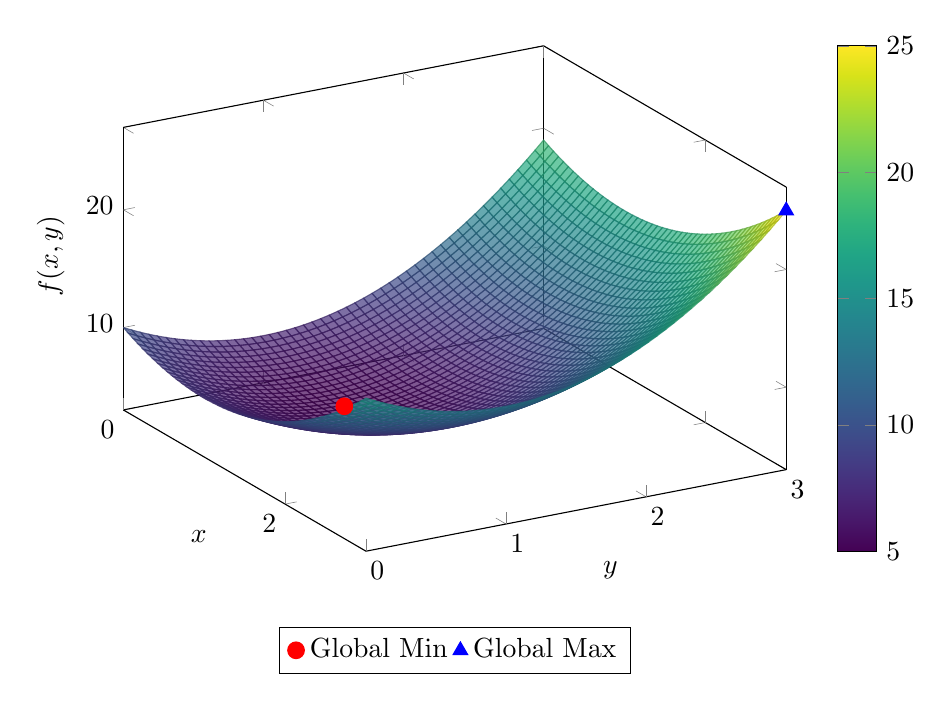
\begin{tikzpicture}
    \begin{axis}[
        view={60}{30},
        xlabel={$x$},
        ylabel={$y$},
        zlabel={$f(x,y)$},
        domain=0:3,
        y domain=0:3,
        samples=50,
        samples y=50,
        colormap/viridis,
        colorbar,
        width=10cm,
        height=8cm,
        legend style={at={(0.5,-0.15)}, anchor=north, legend columns=2},
    ]
    % Surface Plot (without legend)
    \addplot3[
        surf,
        opacity=0.7,
        forget plot,
    ]
    {2*x^2 + 3*y^2 - 4*x - 6*y + 10};
    
    % Plot the global minimum point with red circle
    \addplot3[
        only marks,
        mark=*,
        mark size=3pt,
        color=red,
    ]
    coordinates {(1,1,5)};
    \addlegendentry{Global Min}
    
    % Plot the global maximum point with blue triangle
    \addplot3[
        only marks,
        mark=triangle*,
        mark size=3pt,
        color=blue,
    ]
    coordinates {(3,3,25)};
    \addlegendentry{Global Max}
    
    \end{axis}
\end{tikzpicture}
\end{center}

\noindent The plot above illustrates the function \( f(x,y) = 2x^2 + 3y^2 - 4x - 6y + 10 \) over the region \( R \). The global minimum at \( (1, 1, 5) \) is marked with a \textbf{red circle}, and the global maximum at \( (3, 3, 25) \) with a \textbf{blue triangle}. Refer to the legend below the graph for clarification.
    \end{solution}
\end{example}
\exampleline

\subsection*{Saddle Points: A New Category of Critical Points} \index{Saddle Points} 

\noindent We've danced around it throughout this chapter, but we are now going to formally define it...in single-variable calculus, if \( f'(a)=0 \) and \( f''(a)=0 \), you might get a point of inflection. Inflection points are where the function’s curvature changes sign. In multiple dimensions, we have a richer phenomenon: the \textbf{saddle point}. \\

\noindent A saddle point is a critical point that is not a maximum or a minimum. Think of a horse saddle: at the saddle’s center, if you move forward and backward along the horse's spine, you might go up; but if you move left and right across the saddle, you might go down. The point is neither a peak nor a valley—some directions lead you higher, others lead you lower. Mathematically, this corresponds to the Hessian being indefinite at that point.

% Insert a schematic figure for a saddle point
\begin{figure}[H]
\centering
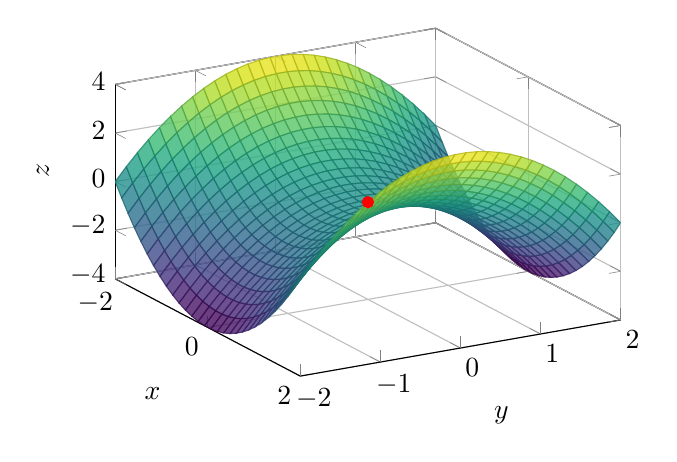
\begin{tikzpicture}
  \begin{axis}[
    view={60}{30}, 
    xlabel={$x$}, ylabel={$y$}, zlabel={$z$},
    domain=-2:2, y domain=-2:2,
    samples=30, samples y=30,
    width=8cm, height=6cm,
    grid=major,
    colormap/viridis,
    zmin=-4, zmax=4
  ]
  % Example saddle surface: z = x^2 - y^2
  \addplot3[surf, opacity=0.8] {x^2 - y^2};
  \addplot3[mark=*, color=red] coordinates {(0,0,0)};
  \end{axis}
\end{tikzpicture}
\caption{\textit{A saddle point at \((0,0)\) for the function \(z=x^2-y^2.\) Along the \(x\)-axis, the function looks like a minimum; along the \(y\)-axis, it looks like a maximum. Overall, it's neither, defining a classic saddle shape.}}
\end{figure}

\noindent In the example above, the function \( f(x,y)=x^2-y^2 \) has a critical point at \((0,0)\). Checking the criteria:
\[
f_{xx}=2,\quad f_{yy}=-2,\quad f_{xy}=0.
\]
Therefore we have $D = 2(-2) - (0^2) = -4 < 0$. Thus, confirming a saddle point. Our previous example we saw in Figure~\ref{fig:extrema_ex} the origin is a saddle point. Let's find it!


\exampleline
\begin{example} Determine the saddle point of the function \( f(x,y) = \sin(x)\sin(y)e^{-0.1(x^2 + y^2)} \).
    
  \begin{solution}
    \begin{enumerate}
        \item \textbf{Identify Critical Points:}
        
        \begin{itemize}
            \item First Partial Derivatives:
            \[
            f_x = \sin(y)e^{x^2 + y^2}(\cos(x) + 2x\sin(x)), \quad 
            f_y = \sin(x)e^{x^2 + y^2}(\cos(y) + 2y\sin(y)).
            \]
            
            \item Setting \( f_x = 0 \) and \( f_y = 0 \):
            \[
            \sin(y) = 0 \quad \text{or} \quad \cos(x) + 2x\sin(x) = 0,
            \]
            \[
            \sin(x) = 0 \quad \text{or} \quad \cos(y) + 2y\sin(y) = 0.
            \]
            
            \item Critical Point:
            \[
            (x, y) = (0, 0).
            \]
        \end{itemize}
        
        \item \textbf{Classify the Critical Point Using the Second Derivative Test:}
        
        \begin{itemize}
            \item Second Partial Derivatives at \( (0,0) \):
            \[
            f_{xx} = 0, \quad f_{yy} = 0, \quad f_{xy} = 1.
            \]
            
            \item Discriminant Calculation:
            \[
            D = f_{xx}f_{yy} - (f_{xy})^2 = (0)(0) - (1)^2 = -1 < 0.
            \]
            
            \item Classification:
            \begin{itemize}
                \item Since \( D < 0 \), the critical point \( (0, 0) \) is a \textbf{saddle point}.
            \end{itemize}
        \end{itemize}
    \end{enumerate}
  
\end{solution}
\end{example}
\exampleline


\subsection*{Generalization to \( n \)-Variables and the Hessian Matrix} \index{Hessian Matrix} 

\noindent For functions \( f: \mathbb{R}^n \to \mathbb{R} \), the second derivative test uses the \textbf{Hessian matrix}, an \( n \times n \) matrix of second partial derivatives:
\[
H(\mathbf{a}) = \begin{bmatrix}
f_{x_1x_1}(\mathbf{a}) & f_{x_1x_2}(\mathbf{a}) & \cdots & f_{x_1x_n}(\mathbf{a}) \\[5pt]
f_{x_2x_1}(\mathbf{a}) & f_{x_2x_2}(\mathbf{a}) & \cdots & f_{x_2x_n}(\mathbf{a}) \\[5pt]
\vdots & \vdots & \ddots & \vdots \\[5pt]
f_{x_nx_1}(\mathbf{a}) & f_{x_nx_2}(\mathbf{a}) & \cdots & f_{x_nx_n}(\mathbf{a})
\end{bmatrix}.
\]

\noindent The two-variable discriminant \( D \) is just the determinant of the \( 2 \times 2 \) Hessian for \( n=2 \). For higher dimensions, determining whether a critical point is a local maximum, minimum, or saddle point involves examining the \textbf{definiteness} of the Hessian matrix. This is where the concepts of positive definite, negative definite, indefinite, and semidefinite come into play.

\noindent To understand these terms, we first introduce the concept of eigenvalues:

\begin{itemize}
  \item \textbf{Eigenvalues:} Mathematically, an eigenvalue \( \lambda \) of a square matrix \( A \) is a scalar such that there exists a nonzero vector \( \mathbf{v} \) (called an eigenvector) satisfying the equation:
  \[
  A \mathbf{v} = \lambda \mathbf{v}.
  \]
  In this equation, the matrix \( A \) acts on the eigenvector \( \mathbf{v} \), and the result is the same as scaling \( \mathbf{v} \) by \( \lambda \). To find eigenvalues, we solve the characteristic equation:
  \[
  \det(A - \lambda I) = 0,
  \]
  where \( I \) is the identity matrix. The eigenvalues of the Hessian matrix \( H \) provide insight into the curvature of the function in specific directions. Positive eigenvalues correspond to upward curvature (like a local minimum), while negative eigenvalues correspond to downward curvature (like a local maximum). Mixed signs indicate the presence of a saddle point.
\end{itemize}

\noindent The definiteness of the Hessian matrix is determined by the signs of its eigenvalues: \index{Matrix Definiteness}  \index{Eigenvalues} 

\begin{itemize}
    \item \textbf{Positive Definite Hessian:} \index{Positive Definiteness} 
    \begin{itemize}
        \item All eigenvalues of the Hessian are positive.
        \item Implication: The function curves upwards in all directions around the critical point, indicating a \textbf{local minimum}.
    \end{itemize}
    
    \item \textbf{Negative Definite Hessian:} \index{Negative Definiteness} 
    \begin{itemize}
        \item All eigenvalues of the Hessian are negative.
        \item Implication: The function curves downwards in all directions around the critical point, indicating a \textbf{local maximum}.
    \end{itemize}
    
    \item \textbf{Indefinite Hessian:} \index{Indefiniteness} 
    \begin{itemize}
        \item The Hessian has both positive and negative eigenvalues.
        \item Implication: The function curves upwards in some directions and downwards in others around the critical point, indicating a \textbf{saddle point}.
    \end{itemize}
    
    \item \textbf{Semidefinite Hessian:} \index{Semidefiniteness} 
    \begin{itemize}
        \item The Hessian has eigenvalues that are all non-negative or all non-positive, but not all strictly positive or negative.
        \item Implication: The test is \textbf{inconclusive}, and further analysis is required to classify the critical point.
    \end{itemize}
\end{itemize}

\noindent While the linear algebra underlying definiteness and eigenvalues is more advanced, the key takeaway is that the Hessian matrix generalizes the notion of the second derivative test to any dimension. In two dimensions, the discriminant \( D = \det(H) \) and the sign of \( f_{xx}(a,b) \) provide a simpler, more direct criterion for classifying critical points.\\

\noindent Recall that we saw for a \( 2 \times 2 \) Hessian matrix:
\[
H = \begin{bmatrix}
f_{xx} & f_{xy} \\
f_{yx} & f_{yy}
\end{bmatrix},
\]
the discriminant \( D \) is calculated as:
\[
D = f_{xx}f_{yy} - (f_{xy})^2.
\]

\noindent  Now with higher dimensions,  we need to discuss the definiteness of the Hessian in terms of classifying critical points:
\begin{itemize}
    \item If \( D > 0 \) and \( f_{xx} > 0 \), the Hessian is \textbf{positive definite}, indicating a \textbf{local minimum}.
    \item If \( D > 0 \) and \( f_{xx} < 0 \), the Hessian is \textbf{negative definite}, indicating a \textbf{local maximum}.
    \item If \( D < 0 \), the Hessian is \textbf{indefinite}, indicating a \textbf{saddle point}.
    \item If \( D = 0 \), the Hessian is \textbf{semidefinite}, and the test is \textbf{inconclusive}.
\end{itemize}
\noindent Let's move up a dimension. When we consider a function of three variables, \( w = f(x,y,z) \), we will have more combinations of second derivatives and thus our Hessian will be:

\[
H = \begin{bmatrix}
f_{xx} & f_{xy} & f_{xz} \\[5pt]
f_{yx} & f_{yy} & f_{yz} \\[5pt]
f_{zx} & f_{zy} & f_{zz}
\end{bmatrix}.
\]

\noindent This will result in a more complicated discriminant:

\[
D = \det(H) = f_{xx}(f_{yy}f_{zz} - f_{yz}^2) - f_{xy}(f_{yx}f_{zz} - f_{yz}f_{zx}) + f_{xz}(f_{yx}f_{zy} - f_{yy}f_{zx}).
\]
\noindent The the criteria for a function of three variables gets a little more complicated: we first examine the structure of the Hessian and the determinant of the \( 2 \times 2 \) upper-left submatrix, which corresponds to the case of two variables. This submatrix is:

\[
H_2 = \begin{bmatrix}
f_{xx} & f_{xy} \\[5pt]
f_{yx} & f_{yy}
\end{bmatrix},
\]
and its determinant is given by:
\[
D_2 = \det(H_2) = f_{xx}f_{yy} - (f_{xy})^2.
\]

\noindent For a function of three variables, the \textbf{leading principal minors} \index{Leading Principal Minors}  are \( D_1 \), \( D_2 \), and \( D_3 \), where:
\begin{itemize}
    \item \( D_1 = f_{xx} \),
    \item \( D_2 = \det(H_2) = f_{xx}f_{yy} - (f_{xy})^2 \),
    \item \( D_3 = \det(H) \), the determinant of the full \( 3 \times 3 \) Hessian.
\end{itemize}

\noindent The criteria for definiteness in three dimensions are:
\begin{itemize}
    \item If \( D_3 > 0 \), \( D_2 > 0 \), and \( D_1 > 0 \), the Hessian is \textbf{positive definite}, indicating a \textbf{local minimum}.
    \item If \( D_3 < 0 \), \( D_2 > 0 \), and \( D_1 < 0 \), the Hessian is \textbf{negative definite}, indicating a \textbf{local maximum}.
    \item If the leading principal minors do not satisfy either the positive definite or negative definite conditions, the Hessian is \textbf{indefinite}, indicating a \textbf{saddle point}.
    \item If any leading principal minor \( D_k = 0 \), the test is inconclusive and further analysis is required.
\end{itemize}

\noindent Let us now extend this reasoning to \( n \)-dimensional functions. For a function \( f(\mathbf{x}) \), where \( \mathbf{x} = (x_1, x_2, \dots, x_n) \), the Hessian is an \( n \times n \) matrix:

\[
H = \begin{bmatrix}
f_{x_1x_1} & f_{x_1x_2} & \cdots & f_{x_1x_n} \\[5pt]
f_{x_2x_1} & f_{x_2x_2} & \cdots & f_{x_2x_n} \\[5pt]
\vdots & \vdots & \ddots & \vdots \\[5pt]
f_{x_nx_1} & f_{x_nx_2} & \cdots & f_{x_nx_n}
\end{bmatrix}.
\]

\noindent The determinant of the Hessian for \( n \)-dimensions is given by:
\[
D_n = \det(H).
\]

\noindent The criteria for definiteness are generalized using \textbf{Sylvester's Criterion}, \index{Sylvester's Criterion} which states:
\begin{itemize}
    \item The Hessian is \textbf{positive definite} (indicating a local minimum) if all leading principal minors are positive:
    \[
    D_1 > 0, \quad D_2 > 0, \quad \dots, \quad D_n > 0.
    \]
    \item The Hessian is \textbf{negative definite} (indicating a local maximum) if the leading principal minors alternate in sign, starting with \( D_1 < 0 \):
    \[
    D_1 < 0, \quad D_2 > 0, \quad D_3 < 0, \quad \dots, \quad D_n \text{ has sign } (-1)^n.
    \]
    \item The Hessian is \textbf{indefinite} (indicating a saddle point) if the sequence of leading principal minors does not satisfy the conditions for positive or negative definiteness.
    \item The Hessian is \textbf{semidefinite} if one or more leading principal minors are zero, and the remaining minors satisfy the conditions for definiteness.
\end{itemize}

\noindent Sylvester's Criterion provides a systematic method to evaluate the definiteness of the Hessian for functions of any dimension, extending the utility of the second derivative test to higher-dimensional problems. \\

\noindent This framework allows us to extend the second derivative test from single-variable calculus to functions of multiple variables, enabling the classification of critical points in higher dimensions.


\newpage

\lecture{Optimization}

\noindent In the previous lecture, we developed tools for identifying and classifying extrema of multivariable functions, analyzing both local and global extrema using critical points and the Hessian matrix. These methods extended single-variable concepts to multiple dimensions, allowing us to handle optimization problems in unconstrained settings -- indeed, we implicitly handled unconstrained optimization to a large degree by carefully and deeply examining extrema. However, real-world optimization problems often involve constraints: limits imposed by resources, boundaries, or conditions that must be satisfied. This lecture introduces techniques for optimization in constrained settings, starting with Lagrange multipliers and culminating in a discussion on how these methods generalize to applications in fields such as machine learning.

\begin{figure}[H]
    \centering
    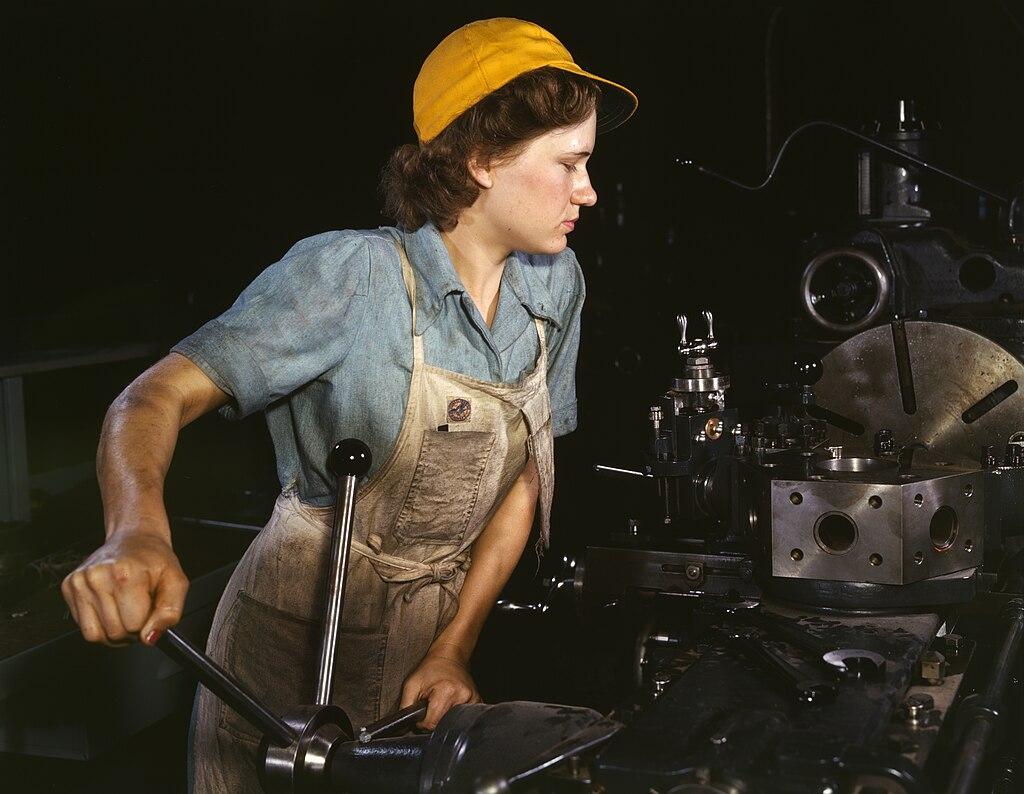
\includegraphics[width=0.45\textwidth]{chapters/chp3_pics/Factory.jpg}
\caption{\textit{Manufacturing is the foremost application of optimization in our day-to-day lives. You may even have noticed what is called `Shrinkflation': goods being shrunken down with a higher price. This is due to cost optimization.}}
    \label{fig:factory}
\end{figure}

%https://commons.wikimedia.org/wiki/File:WomanFactory1940s.jpg


\subsection*{Unconstrained Optimization} \index{Unconstrained Optimization}

\noindent Optimization is a cornerstone of mathematics, embodying the search for maxima and minima—points where a function reaches its highest or lowest values. These principles permeate problems across science, engineering, and economics, where achieving efficiency or minimizing costs is a primary objective. In this lecture, we dig deeper into the concepts of extrema by clarifying them with an applied nature. As we shift toward constrained optimization, it is essential to reflect on the foundational tools of \textit{unconstrained optimization}, which underlie more intricate scenarios. \\

\noindent Recall from our earlier discussions that the key to finding extrema lies in identifying points where the behavior of a function undergoes a qualitative change. For a differentiable function \( f: \mathbb{R}^n \to \mathbb{R} \), such points—termed \textbf{critical points}—are characterized by the condition:
\[
\nabla f(\mathbf{x}) = \mathbf{0}.
\]
At these points, the gradient, which represents the direction of steepest ascent, becomes zero, signaling that the function is momentarily stationary. Yet as we learned, not all critical points correspond to maxima or minima. Some may represent \textit{saddle points}, where the function exhibits an increase in certain directions and a decrease in others. This necessitated a framework for systematically classifying critical points.

\noindent The tools we have developed for this classification are summarized below:
\begin{enumerate}
    \item \textbf{The Gradient Condition:} Critical points are identified by solving \( \nabla f(\mathbf{x}) = \mathbf{0} \). This forms the foundation for locating potential extrema.

    \item \textbf{The Second Derivative Test:} Once critical points are located, the nature of each point is determined by examining the \textbf{Hessian matrix} \( H(\mathbf{x}) \), the matrix of second partial derivatives of \( f \). For two-variable functions, the determinant of the Hessian, denoted as \( D \), provides a straightforward method for classification:
    \[
    D = f_{xx} f_{yy} - (f_{xy})^2.
    \]
    The following rules apply:
    \begin{itemize}
        \item If \( D > 0 \) and \( f_{xx} > 0 \), the point is a local minimum.
        \item If \( D > 0 \) and \( f_{xx} < 0 \), the point is a local maximum.
        \item If \( D < 0 \), the point is neither a maximum nor a minimum and is instead a saddle point.
        \item If \( D = 0 \), the test is inconclusive, requiring further analysis.
    \end{itemize}

    \item \textbf{Boundary Analysis:} For functions defined on bounded domains, extrema may occur on the boundary. This requires evaluating \( f \) along the domain's boundary in addition to examining critical points within the interior.
\end{enumerate}

\noindent Together, these tools provide a comprehensive framework for unconstrained optimization. By systematically identifying and classifying critical points and incorporating boundary conditions where necessary, we can thoroughly analyze the behavior of a function over its domain. \\

\noindent It is worth emphasizing that unconstrained optimization closely mirrors the techniques we have already mastered. The interplay between geometry and calculus is a recurring theme: the condition \( \nabla f = \mathbf{0} \) encapsulates the geometric intuition that the gradient vanishes at extrema, while the second derivative test provides a quantitative measure of curvature. This shared foundation ensures a seamless transition into more advanced topics, as the principles of unconstrained optimization naturally extend to problems involving constraints.


\exampleline
\begin{example}
A company wants to minimize the cost of manufacturing a product. The cost function is given by 
\[
f(x, y) = x^2 + y^2 - 4x - 6y + 13,
\]
where \(x\) and \(y\) represent two key factors influencing production efficiency. Determine the optimal values of \(x\) and \(y\) to achieve the minimum cost.

\begin{solution}
This is an unconstrained optimization problem because there are no restrictions on the values \(x\) and \(y\) can take. Solving this involves finding the extrema of \(f(x, y)\), which simplifies to finding the minimum.

\begin{enumerate}
    \item \textbf{Identify Critical Points:}
    \begin{itemize}
        \item Compute the gradient of \(f\):
        \[
        \nabla f = \begin{bmatrix} \frac{\partial f}{\partial x} \\ \frac{\partial f}{\partial y} \end{bmatrix} = \begin{bmatrix} 2x - 4 \\ 2y - 6 \end{bmatrix}.
        \]
        \item Set \( \nabla f = \mathbf{0} \) to find critical points:
        \[
        2x - 4 = 0 \quad \text{and} \quad 2y - 6 = 0.
        \]
        Solving these equations gives \( x = 2 \) and \( y = 3 \). Thus, the critical point is \( (2, 3) \).
    \end{itemize}

    \item \textbf{Classify the Critical Point Using the Second Derivative Test:}
    \begin{itemize}
        \item Compute the Hessian matrix \(H\):
        \[
        H = \begin{bmatrix} 
        \frac{\partial^2 f}{\partial x^2} & \frac{\partial^2 f}{\partial x \partial y} \\ 
        \frac{\partial^2 f}{\partial y \partial x} & \frac{\partial^2 f}{\partial y^2} 
        \end{bmatrix} = \begin{bmatrix} 
        2 & 0 \\ 
        0 & 2 
        \end{bmatrix}.
        \]
        \item Calculate the determinant of \(H\):
        \[
        D = \frac{\partial^2 f}{\partial x^2} \cdot \frac{\partial^2 f}{\partial y^2} - \left( \frac{\partial^2 f}{\partial x \partial y} \right)^2 = (2)(2) - (0)^2 = 4 > 0.
        \]
        \item Since \(D > 0\) and \( \frac{\partial^2 f}{\partial x^2} = 2 > 0 \), the critical point \( (2, 3) \) is a \textbf{local minimum}.
    \end{itemize}

    \item \textbf{Evaluate the Function at the Critical Point:}
    \begin{itemize}
        \item Substituting \(x = 2\) and \(y = 3\) into \(f(x, y)\):
        \[
        f(2, 3) = (2)^2 + (3)^2 - 4(2) - 6(3) + 13 = 4 + 9 - 8 - 18 + 13 = 0.
        \]
        \item The minimum cost is \(0\), achieved when \(x = 2\) and \(y = 3\).
    \end{itemize}
\end{enumerate}
\end{solution}
\end{example}
\exampleline


\noindent This simple example reinforces the utility of these methods and foreshadows their extensions to more complex scenarios.

\subsubsection*{Classical Examples of Unconstrained Optimization}

\noindent The classical examples we explore highlight the versatility of unconstrained optimization in various settings. For each, we provide a commonly optimized formula to solidify the connection to practical applications:

\begin{enumerate}
    \item \textbf{Economic Models:} 
    \begin{itemize}
        \item Profit Maximization: Optimize the profit function \( P = R - C \), where \( R \) is revenue and \( C \) is cost.
        \item Cost Minimization: Minimize \( C(q) \), where \( C \) is the cost function and \( q \) is the quantity of goods or services produced.
    \end{itemize}
    
    \item \textbf{Physics Applications:} 
    \begin{itemize}
        \item Potential Energy Minimization: Minimize \( U = \frac{1}{2}kx^2 \), the potential energy of a spring system, where \( k \) is the spring constant and \( x \) is the displacement.
        \item Kinetic Energy Optimization: Maximize \( K = \frac{1}{2}mv^2 \), where \( m \) is mass and \( v \) is velocity.
    \end{itemize}
    
    \item \textbf{Machine Learning:} 
    \begin{itemize}
        \item Loss Function Minimization: Minimize a loss function \( L(w) = \frac{1}{N} \sum_{i=1}^N (y_i - f(x_i, w))^2 \), where \( w \) is the parameter vector, \( (x_i, y_i) \) are data points, and \( f \) is the model.
    \end{itemize}
    
    \item \textbf{Geometric Optimization:} \index{Geometric Optimization}
    \begin{itemize}
        \item Volume of a Box: Maximize \( V = l \cdot w \cdot h \), where \( l \), \( w \), and \( h \) are length, width, and height.
        \item Volume of a Sphere: Maximize \( V = \frac{4}{3}\pi r^3 \), where \( r \) is the radius.
        \item Volume of a Cylinder: Maximize \( V = \pi r^2 h \), where \( r \) is the radius and \( h \) is the height.
        \item Solids of Revolution: Optimize the volume \( V = \pi \int_a^b [f(x)]^2 \, dx \), where \( f(x) \) is the curve being rotated about an axis.
    \end{itemize}
\end{enumerate}

\noindent These examples provide a foundation for solving unconstrained optimization problems across disciplines. Each formula highlights a tangible objective, whether maximizing profit, minimizing energy, training a machine learning model, or optimizing the geometry of an object. Geometric optimization, in particular, lays the groundwork for exploring practical shapes and volumes used in design and engineering.

\exampleline
\begin{example}
Find the maximum volume of a rectangular box with its base in the \(xy\)-plane and its top lying on the plane \( z = 12 - 2x - 3y \) in the first octant.

\begin{solution}
\begin{enumerate}
    \item \textbf{Formulate the Volume Function:}
    
    \begin{itemize}
        \item The base of the box lies in the \(xy\)-plane, and its top touches the plane \( z = 12 - 2x - 3y \).
        \item The dimensions of the box are \( x \), \( y \), and \( z \), where \( z \) is given by the equation of the plane.
        \item The volume of the box is:
        \[
        V = x \cdot y \cdot z = x \cdot y \cdot (12 - 2x - 3y).
        \]
        Expand this expression:
        \[
        V(x, y) = 12xy - 2x^2y - 3xy^2.
        \]
    \end{itemize}

    \item \textbf{Find the Critical Points:}
    
    \begin{itemize}
        \item Compute the partial derivatives of \( V \):
        \[
        V_x = \frac{\partial V}{\partial x} = 12y - 4xy - 3y^2,
        \]
        \[
        V_y = \frac{\partial V}{\partial y} = 12x - 2x^2 - 6xy.
        \]
        \item Set \( V_x = 0 \) and \( V_y = 0 \):
        \[
        12y - 4xy - 3y^2 = 0 \quad \text{(1)},
        \]
        \[
        12x - 2x^2 - 6xy = 0 \quad \text{(2)}.
        \]
        Factor equation (1):
        \[
        y(12 - 4x - 3y) = 0.
        \]
        Thus, \( y = 0 \) or \( 12 - 4x - 3y = 0 \), giving \( y = \frac{12 - 4x}{3} \).

        Factor equation (2):
        \[
        x(12 - 2x - 6y) = 0.
        \]
        Thus, \( x = 0 \) or \( 12 - 2x - 6y = 0 \), giving \( y = \frac{12 - 2x}{6} = 2 - \frac{x}{3} \).

        \item Solve the system of equations:
        Substituting \( y = \frac{12 - 4x}{3} \) into \( y = 2 - \frac{x}{3} \):
        \[
        \frac{12 - 4x}{3} = 2 - \frac{x}{3}.
        \]
        Multiply through by 3:
        \[
        12 - 4x = 6 - x \quad \Rightarrow \quad 3x = 6 \quad \Rightarrow \quad x = 2.
        \]
        Substitute \( x = 2 \) into \( y = 2 - \frac{x}{3} \):
        \[
        y = 2 - \frac{2}{3} = \frac{6}{3} - \frac{2}{3} = \frac{4}{3}.
        \]
    \end{itemize}

    \item \textbf{Classify the Critical Point and Find the Volume:}
    
    The critical point is \( (x, y) = (2, \frac{4}{3}) \). At this point:
    \[
    z = 12 - 2x - 3y = 12 - 2(2) - 3\left(\frac{4}{3}\right) = 12 - 4 - 4 = 4.
    \]
    The dimensions of the box are \( x = 2 \), \( y = \frac{4}{3} \), and \( z = 4 \).
    \[
    V = x \cdot y \cdot z = 2 \cdot \frac{4}{3} \cdot 4 = \frac{32}{3}.
    \]
    Since \( V = 0 \) on the boundary of the first-octant region (where \( x = 0 \), \( y = 0 \), or \( z = 0 \)) and \( V > 0 \) at the interior critical point, this critical point must yield the maximum volume.

\end{enumerate}
\end{solution}
\end{example}
\exampleline


\subsection*{Optimization with Equality Constraints} \index{Constrained Optimization}

\noindent Consider the task of optimizing a function \( f(x, y) \) subject to a constraint \( g(x, y) = c \), where \( g \) is a differentiable function that defines a curve or surface in \( \mathbb{R}^n \). This problem can be visualized as finding the highest or lowest point on the curve or surface defined by \( g(x, y) = c \), rather than across the entire plane or space. To solve this, we introduce the method of \textbf{Lagrange multipliers}. \\

\noindent To build intuition, recall that the gradient \( \nabla g(x, y) \) of the constraint function points in the direction of the steepest ascent of \( g(x, y) \). The curve \( g(x, y) = c \) represents a level set of \( g \), and at any point along this curve, \( \nabla g(x, y) \) is normal to the curve. Similarly, the gradient \( \nabla f(x, y) \) of the objective function \( f(x, y) \) indicates the direction of steepest ascent of \( f \). At an extremum of \( f \) constrained to \( g(x, y) = c \), these gradients must align, meaning \( \nabla f(x, y) \) must point in the same or opposite direction as \( \nabla g(x, y) \).

\noindent This condition is expressed mathematically as:
\[
\nabla f(x, y) = \lambda \nabla g(x, y),
\]
where \( \lambda \) is a scalar known as the \textbf{Lagrange multiplier} \index{Lagrange Multiplier}. The scalar \( \lambda \) measures how much the objective function \( f \) changes per unit increase in the constraint \( g \).

\subsubsection*{The Lagrange Condition} \index{Lagrange Condition}

\noindent To derive this condition, consider the constrained optimization problem as finding the extrema of \( f(x, y) \) on the curve \( g(x, y) = c \). We construct the \textit{Lagrangian}: \index{Lagrange Function}
\[
\mathcal{L}(x, y, \lambda) = f(x, y) - \lambda \big(g(x, y) - c\big).
\]
\noindent The term \( \lambda(g(x, y) - c) \) enforces the constraint \( g(x, y) = c \). At the extrema of \( f(x, y) \) subject to this constraint, the gradients of \( \mathcal{L} \) with respect to \( x \), \( y \), and \( \lambda \) must vanish:
\[
\frac{\partial \mathcal{L}}{\partial x} = \frac{\partial f}{\partial x} - \lambda \frac{\partial g}{\partial x} = 0, \quad
\frac{\partial \mathcal{L}}{\partial y} = \frac{\partial f}{\partial y} - \lambda \frac{\partial g}{\partial y} = 0, \quad
\frac{\partial \mathcal{L}}{\partial \lambda} = -(g(x, y) - c) = 0.
\]
\noindent These equations are equivalent to the system:
\[
\begin{aligned}
    \nabla f(x, y) - \lambda \nabla g(x, y) &= \mathbf{0}, \\
    g(x, y) &= c.
\end{aligned}
\]

\noindent The first equation ensures that \( \nabla f \) and \( \nabla g \) are parallel (aligned with \( \lambda \)), while the second equation enforces the constraint. Thus, the optimization problem reduces to solving this system of equations for \( x \), \( y \), and \( \lambda \). \\

\noindent To solve an optimization problem using Lagrange multipliers:
\begin{enumerate}
    \item Compute \( \nabla f(x, y) \) and \( \nabla g(x, y) \).
    \item Set up the system of equations:
    \[
    \nabla f(x, y) - \lambda \nabla g(x, y) = \mathbf{0}, \quad g(x, y) = c.
    \]
    \item Solve the system for \( x \), \( y \), and \( \lambda \).
    \item Evaluate \( f(x, y) \) at the solutions to determine the extrema.
\end{enumerate}

\noindent The equation \( \nabla f = \lambda \nabla g \) has a powerful geometric interpretation. Recall that \( \nabla g(x, y) \) is orthogonal to the level curve \( g(x, y) = c \) at any point. Similarly, \( \nabla f(x, y) \) is orthogonal to the level curve of \( f(x, y) \). Thus, the condition \( \nabla f = \lambda \nabla g \) implies that the level curves of \( f \) and \( g \) are tangent at the optimal point. This tangency ensures that \( f(x, y) \) is extremized subject to the constraint \( g(x, y) = c \).

\exampleline
\begin{example}
Find the minimum of the function \( f(x, y) = x^2 + y^2 \) subject to the constraint \( x + y = 2 \).

\begin{solution}
\begin{enumerate}
    \item \textbf{Formulate the Lagrangian:}
    
    To apply the method of Lagrange multipliers, we introduce a Lagrange multiplier \( \lambda \) and construct the Lagrangian function:
    \[
    \mathcal{L}(x, y, \lambda) = f(x, y) - \lambda (g(x, y) - c),
    \]
    where \( g(x, y) = x + y \) and \( c = 2 \).
    
    Substituting the given functions:
    \[
    \mathcal{L}(x, y, \lambda) = x^2 + y^2 - \lambda (x + y - 2).
    \]
    
    \item \textbf{Compute the Partial Derivatives:}
    
    To find the extrema, take the partial derivatives of \( \mathcal{L} \) with respect to \( x \), \( y \), and \( \lambda \), and set them equal to zero.
    
    \begin{itemize}
        \item \textbf{Partial derivative with respect to \( x \):}
        \[
        \frac{\partial \mathcal{L}}{\partial x} = 2x - \lambda = 0 \quad \Rightarrow \quad \lambda = 2x \quad (1)
        \]
        
        \item \textbf{Partial derivative with respect to \( y \):}
        \[
        \frac{\partial \mathcal{L}}{\partial y} = 2y - \lambda = 0 \quad \Rightarrow \quad \lambda = 2y \quad (2)
        \]
        
        \item \textbf{Partial derivative with respect to \( \lambda \):}
        \[
        \frac{\partial \mathcal{L}}{\partial \lambda} = -(x + y - 2) = 0 \quad \Rightarrow \quad x + y = 2 \quad (3)
        \]
    \end{itemize}
    
    \item \textbf{Solve the System of Equations:}
    
    From equations (1) and (2):
    \[
    2x = \lambda \quad \text{and} \quad 2y = \lambda \quad \Rightarrow \quad 2x = 2y \quad \Rightarrow \quad x = y
    \]
    
    Substitute \( x = y \) into equation (3):
    \[
    x + x = 2 \quad \Rightarrow \quad 2x = 2 \quad \Rightarrow \quad x = 1
    \]
    
    Since \( x = y \):
    \[
    y = 1
    \]
    
    Thus, the critical point is \( (x, y) = (1, 1) \).
    
    \item \textbf{Verify the Solution:}
    
    Substitute \( x = 1 \) and \( y = 1 \) back into the objective function:
    \[
    f(1, 1) = (1)^2 + (1)^2 = 1 + 1 = 2
    \]
    
    Therefore, the function \( f(x, y) = x^2 + y^2 \) attains its minimum value of 2 at the point \( (1, 1) \) under the constraint \( x + y = 2 \).
    
    \item \textbf{Visualization:}
    
    To better understand the optimization, let's visualize the objective function, the constraint, and the optimal point.
    
    \begin{figure}[H]
        \centering
        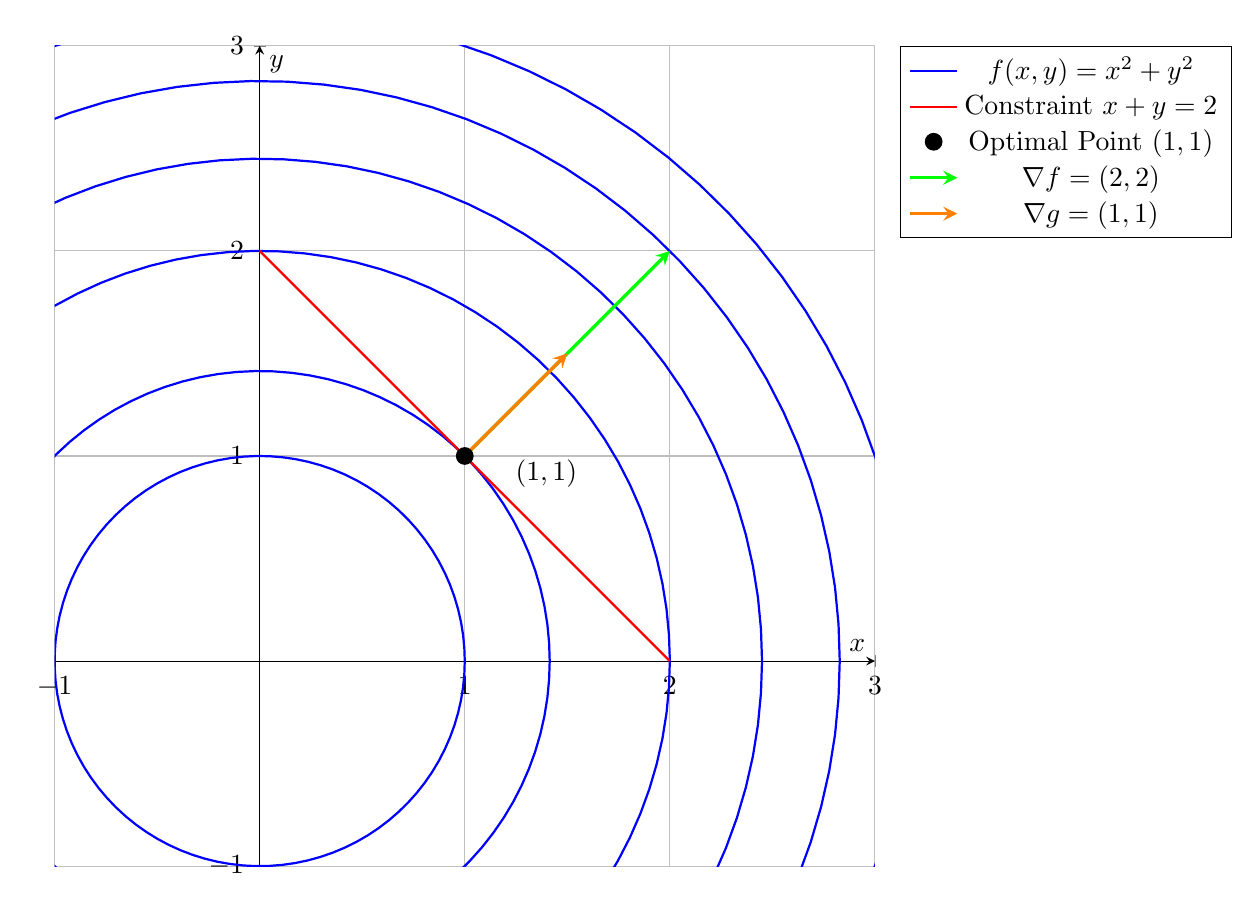
\begin{tikzpicture}
            \begin{axis}[
                xlabel={$x$},
                ylabel={$y$},
                axis lines=middle,
                grid=both,
                minor grid style={gray!25},
                major grid style={gray!50},
                legend pos=outer north east,
                width=12cm,
                height=12cm,
                samples=100, % Increased samples for smoother circles
                domain=0:360, % Angle domain in degrees
                xmin=-1, xmax=3,
                ymin=-1, ymax=3,
                xtick={-1,0,1,2,3},
                ytick={-1,0,1,2,3},
            ]
                % Contour lines for f(x,y) = x^2 + y^2
                \foreach \r in {1,2,4,6,8,10} {
                    \addplot [
                        blue,
                        thick,
                        forget plot % Prevents each contour line from adding to the legend
                    ] 
                        ({sqrt(\r)*cos(\x)}, {sqrt(\r)*sin(\x)});
                }
                % Manually add a single legend entry for the contour lines
                \addlegendimage{blue, thick}
                \addlegendentry{$f(x, y) = x^2 + y^2$}
                
                % Constraint line x + y = 2
                \addplot [
                    red,
                    thick,
                    domain=0:2,
                    samples=2
                ]
                {2 - x};
                \addlegendentry{Constraint $x + y = 2$}
                
                % Optimal point (1,1)
                \addplot[
                    only marks,
                    mark=*,
                    mark size=3pt,
                    black
                ] coordinates {(1,1)};
                \addlegendentry{Optimal Point $(1, 1)$}
                
                % Gradient of f: ∇f = [2x, 2y] at (1,1) => [2,2]
                \addplot[
                    ->,
                    very thick,
                    green,
                    >=stealth
                ] coordinates {(1,1) (1+2*0.5,1+2*0.5)}; % Scaled for visibility
                \addlegendentry{$\nabla f = (2, 2)$}
                
                % Gradient of g: ∇g = [1, 1] at (1,1)
                \addplot[
                    ->,
                    very thick,
                    orange,
                    >=stealth
                ] coordinates {(1,1) (1+1*0.5,1+1*0.5)}; % Scaled for visibility
                \addlegendentry{$\nabla g = (1, 1)$}
                
                % Annotation for the optimal point
                \node at (axis cs:1.2,.8) [anchor=south west] {$(1, 1)$};
            \end{axis}
        \end{tikzpicture}
        \caption{\textit{Visualization of the optimization problem using Lagrange multipliers. The blue circles represent the contour lines of the objective function \( f(x, y) = x^2 + y^2 \), the red line is the constraint \( x + y = 2 \), the black dot marks the optimal point \( (1, 1) \), the green arrow represents the gradient \( \nabla f \), and the orange arrow represents the gradient \( \nabla g \).}}
        \label{fig:lagrange_multiplier_plot_example}
    \end{figure}
    
\end{enumerate}
\end{solution}
\end{example}

\exampleline


\noindent Let's now try a problem that's a little messier and doesn't have a nice answer. We will need to use a computer to solve a polynomial using numerical approximation at the end. This is more representative of a problem you may encounter in an actual professional setting.


\exampleline
\begin{example} Determine the production levels \( x \) and \( y \) for Gadget A and Gadget B, respectively, that minimize the total production cost given by:
\[
C(x, y) = x^2 y + y^3,
\]
subject to the nonlinear constraint:
\[
x^3 + y^3 = 2000.
\]
Since production levels must be integer values, round the approximate solution up or down and choose the option with the lesser cost.

\begin{solution}
\begin{enumerate}
    \item \textbf{Formulate the Lagrangian:}
    
    Introduce a Lagrange multiplier \( \lambda \) and construct the Lagrangian function:
    \[
    \mathcal{L}(x, y, \lambda) = C(x, y) - \lambda (x^3 + y^3 - 2000).
    \]
    Substituting the given functions:
    \[
    \mathcal{L}(x, y, \lambda) = x^2 y + y^3 - \lambda (x^3 + y^3 - 2000).
    \]
    
    \item \textbf{Compute the Partial Derivatives:}
    
    To find the extrema, take the partial derivatives of \( \mathcal{L} \) with respect to \( x \), \( y \), and \( \lambda \), and set them equal to zero.
    
    \begin{itemize}
        \item \textbf{Partial derivative with respect to \( x \):}
        \[
        \frac{\partial \mathcal{L}}{\partial x} = 2xy - 3\lambda x^2 = 0 \quad \Rightarrow \quad 2xy = 3\lambda x^2 \quad (1)
        \]
        
        \item \textbf{Partial derivative with respect to \( y \):}
        \[
        \frac{\partial \mathcal{L}}{\partial y} = x^2 + 3y^2 - 3\lambda y^2 = 0 \quad \Rightarrow \quad x^2 + 3y^2 = 3\lambda y^2 \quad (2)
        \]
        
        \item \textbf{Partial derivative with respect to \( \lambda \):}
        \[
        \frac{\partial \mathcal{L}}{\partial \lambda} = -(x^3 + y^3 - 2000) = 0 \quad \Rightarrow \quad x^3 + y^3 = 2000 \quad (3)
        \]
    \end{itemize}
    
    \item \textbf{Solve the System of Equations:}
    
    From equation (1):
    \[
    2xy = 3\lambda x^2 \quad \Rightarrow \quad \lambda = \frac{2y}{3x} \quad (1a)
    \]
    
    From equation (2):
    \[
    x^2 + 3y^2 = 3\lambda y^2 \quad \Rightarrow \quad \lambda = \frac{x^2 + 3y^2}{3y^2} = \frac{x^2}{3y^2} + 1 \quad (2a)
    \]
    
    Equate the two expressions for \( \lambda \):
    \[
    \frac{2y}{3x} = \frac{x^2}{3y^2} + 1
    \]
    
    Multiply both sides by \( 3x y^2 \) to eliminate denominators:
    \[
    2y \cdot y^2 = x^3 + 3x y^2
    \]
    \[
    2y^3 = x^3 + 3x y^2 \quad (4)
    \]
    
    From the constraint (3):
    \[
    x^3 + y^3 = 2000 \quad \Rightarrow \quad x^3 = 2000 - y^3 \quad (5)
    \]
    
    Substitute \( x^3 = 2000 - y^3 \) into equation (4):
    \[
    2y^3 = (2000 - y^3) + 3x y^2
    \]
    \[
    2y^3 = 2000 - y^3 + 3x y^2
    \]
    \[
    3x y^2 = 3y^3 - 2000
    \]
    \[
    x y^2 = y^3 - \frac{2000}{3} \quad (6)
    \]
    
    Solve for \( x \):
    \[
    x = \frac{y^3 - \frac{2000}{3}}{y^2} = y - \frac{2000}{3y^2} \quad (7)
    \]
    
    Substitute \( x = y - \frac{2000}{3y^2} \) into the constraint \( x^3 + y^3 = 2000 \):
    \[
    \left(y - \frac{2000}{3y^2}\right)^3 + y^3 = 2000
    \]
    
    This equation is highly complex and does not yield to simple algebraic methods. Therefore, we proceed with an approximate numerical solution. For more detailed computations, refer to the \href{https://www.wolframalpha.com/widgets/view.jsp?id=1451afdfe5a25b2a316377c1cd488883}{Wolfram Alpha Lagrange Multipliers} tool.
    
    \item \textbf{Approximate Solution:}
    
    The approximate solution is:
    \[
    (x, y) \approx (7.04423, 11.8177)
    \]
    
    \item \textbf{Decision on Integer Production Levels:}
    
    Since production levels must be integer values, we consider the nearest integer values to the approximate solution. The four possible combinations are:

    \begin{itemize}
        \item Option 1: \( x = 7 \), \( y = 11 \)
        \[
        x^3 + y^3 = 343 + 1331 = 1674 \leq 2000 \quad (\text{Satisfies the constraint})
        \]
        
        \item Option 2: \( x = 7 \), \( y = 12 \)
        \[
        x^3 + y^3 = 343 + 1728 = 2071 > 2000 \quad (\text{Does not satisfy the constraint})
        \]
        
        \item Option 3: \( x = 8 \), \( y = 11 \)
        \[
        x^3 + y^3 = 512 + 1331 = 1843 \leq 2000 \quad (\text{Satisfies the constraint})
        \]
        
        \item Option 4: \( x = 8 \), \( y = 12 \)
        \[
        x^3 + y^3 = 512 + 1728 = 2240 > 2000 \quad (\text{Does not satisfy the constraint})
        \]
    \end{itemize}
    
    Therefore, only Option 1 and Option 3 satisfy the constraint.
    
    \textbf{Compute the Total Cost for Each Option:}
    \begin{itemize}
        \item Option 1: \( x = 7 \), \( y = 11 \)
        \[
        C(7, 11) = 7^2 \times 11 + 11^3 = 49 \times 11 + 1331 = 539 + 1331 = 1870
        \]
        
        \item Option 3: \( x = 8 \), \( y = 11 \)
        \[
        C(8, 11) = 8^2 \times 11 + 11^3 = 64 \times 11 + 1331 = 704 + 1331 = 2035
        \]
    \end{itemize}
    
    \textbf{Decision:}  
    Choose the production levels that satisfy the constraint and incur the lesser cost. Between Option 1 and Option 3:
    \[
    1870 < 2035
    \]
    
    Therefore, Option 1 (\( x = 7 \), \( y = 11 \)) is the optimal integer production level with a total cost of \$1,870.
    
    \item \textbf{Visualization:}
    
    To better understand the optimization, let's visualize the nonlinear constraint, the approximate optimal point, the integer production options, and their associated costs.
    

\begin{figure}[H]
    \centering
    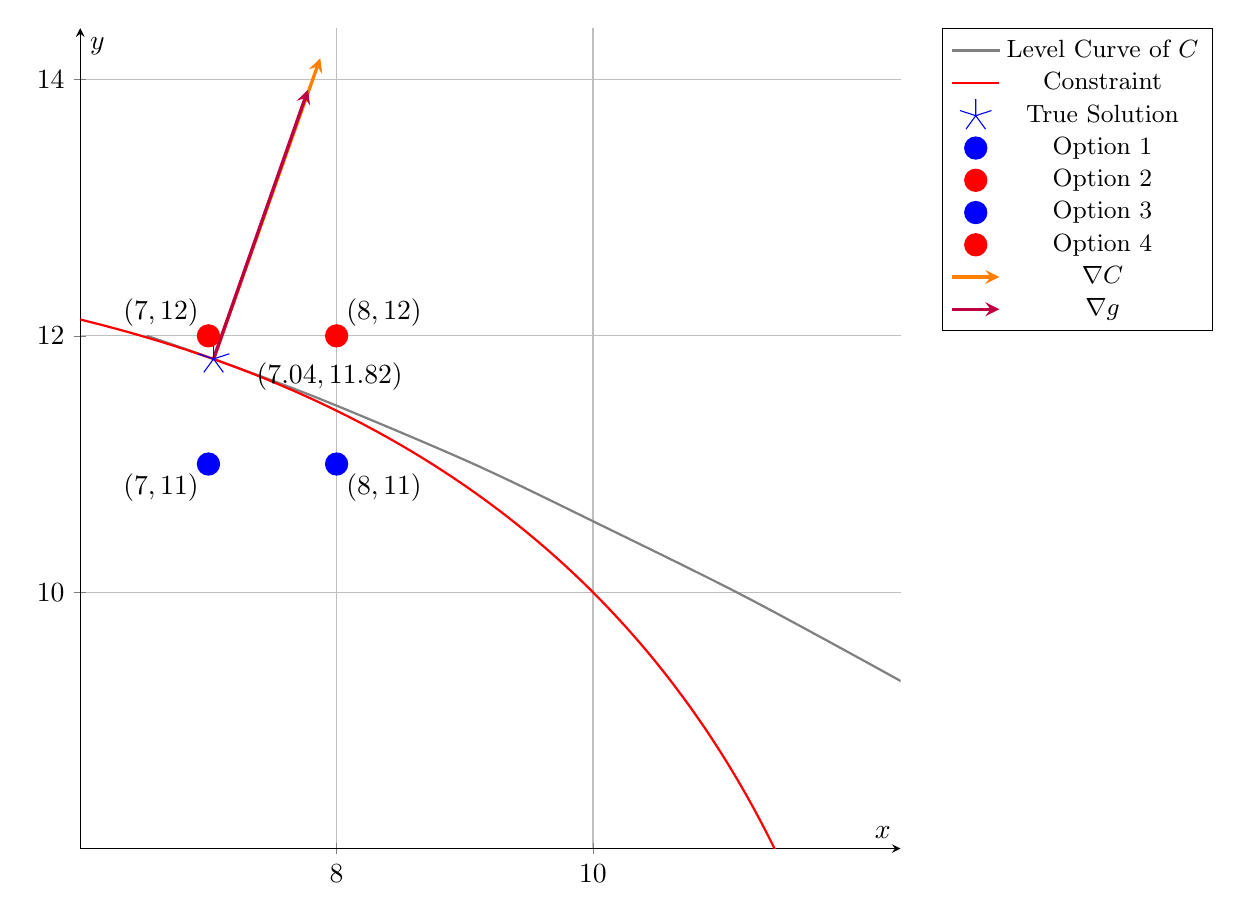
\begin{tikzpicture}
        \begin{axis}[
            xlabel={$x$},
            ylabel={$y$},
            axis lines=middle,
            grid=both,
            minor grid style={gray!25},
            major grid style={gray!50},
            legend style={
                font=\small, 
                at={(1.05,1)}, 
                anchor=north west
            },
            width=12cm,
            height=12cm,
            ymin=8, ymax=14.4, % Adjusted to accommodate y=16.46
            xmin=6, xmax=12.4, % Adjusted to accommodate x=16.46
            xtick={0,2,4,6,8,10},
            ytick={0,2,4,6,8,10,12,14},
        ]
            % Precomputed Level Curve C=2237.10
            \addplot [
                black!50,
                thick,
                smooth,
            ]
                coordinates {
                    (16.46,7)
                    (15.56,7.5)
                    (14.69,8)
                    (13.81,8.5)
                    (12.95,9)
                    (12.05,9.5)
                    (11.12,10)
                    (10.11,10.5)
                    (9.07,11)
                    (7.89,11.5)
                    (7.04,11.82)
                    (6.52,12)
                };
            \addlegendentry{Level Curve of $C$}

            % Nonlinear constraint x^3 + y^3 = 2000
            \addplot [
                red,
                thick,
                domain=6:12, % Adjusted domain to avoid complex numbers
                samples=200,
            ]
                { (2000 - x^3)^(1/3) };
            \addlegendentry{Constraint}

            % Chosen Option: (7.04, 11.82) as a star
            \addplot[
                mark=star,
                mark size=6pt,
                color=blue,
                only marks,
            ] coordinates {(7.04,11.82)};
            \addlegendentry{True Solution}

            % Integer Option 1: (7,11) - Blue Circle (Inside Constraint)
            \addplot[
                only marks,
                mark=*,
                mark size=4pt,
                blue
            ] coordinates {(7,11)};
            \addlegendentry{Option 1}

            % Integer Option 2: (7,12) - Red Circle (Outside Constraint)
            \addplot[
                only marks,
                mark=*,
                mark size=4pt,
                red
            ] coordinates {(7,12)};
            \addlegendentry{Option 2}

            % Integer Option 3: (8,11) - Blue Circle (Inside Constraint)
            \addplot[
                only marks,
                mark=*,
                mark size=4pt,
                blue
            ] coordinates {(8,11)};
            \addlegendentry{Option 3}

            % Integer Option 4: (8,12) - Red Circle (Outside Constraint)
            \addplot[
                only marks,
                mark=*,
                mark size=4pt,
                red
            ] coordinates {(8,12)};
            \addlegendentry{Option 4}

            % Gradient of C: ∇C = [2xy, x^2 + 3y^2] at (7.04,11.82) ≈ [166.52, 469.14]
            % Scaled down by factor 0.005 for visibility
            \addplot[
                ->,
                very thick,
                orange,
                >=stealth
            ] coordinates {
                (7.04,11.82) 
                (7.04 + 166.52*0.005, 11.82 + 469.14*0.005)
            };
            \addlegendentry{$\nabla C$}

            % Gradient of g: ∇g = [3x^2, 3y^2] at (7.04,11.82) ≈ [147.42, 420.0]
            % Scaled down by factor 0.005 for visibility
            \addplot[
                ->,
                very thick,
                purple,
                >=stealth
            ] coordinates {
                (7.04,11.82) 
                (7.04 + 147.42*0.005, 11.82 + 420.0*0.005)
            };
            \addlegendentry{$\nabla g$}

            % Annotations for points
            \node at (axis cs:7.3,11.5) [anchor=south west] {$(7.04, 11.82)$};
            \node at (axis cs:7,11) [anchor=north east] {$(7, 11)$};
            \node at (axis cs:7,12) [anchor=south east] {$(7, 12)$};
            \node at (axis cs:8,11) [anchor=north west] {$(8, 11)$};
            \node at (axis cs:8,12) [anchor=south west] {$(8, 12)$};
        \end{axis}
    \end{tikzpicture}
    \caption{\textit{Visualization of the optimization problem with nonlinear constraint. Red curve: \( x^3 + y^3 = 2000 \). Blue star: Chosen Option \( (7.04, 11.82) \). Blue circles: Options 1 \& 3 (Inside Constraint). Red circles: Options 2 \& 4 (Outside Constraint). Orange arrow: \( \nabla C \). Purple arrow: \( \nabla g \). Level Curve: \( C(x, y) = 2237.10 \).}}
    \label{fig:lagrange_multiplier_complex_example}
\end{figure}


\end{enumerate}
\end{solution}
\end{example}
\exampleline


\subsubsection*{Optimization with Multiple Equality Constraints} \index{Constrained Optimization}

\noindent When optimizing a function \( f(x, y, z) \) subject to two or more equality constraints, such as \( g(x, y, z) = c_1 \) and \( h(x, y, z) = c_2 \), the method of Lagrange multipliers naturally extends to accommodate additional constraints. The underlying principle remains the same: at an optimal point, the gradients of \( f \), \( g \), and \( h \) must align in such a way that any movement satisfying the constraints does not produce a first-order change in \( f \).

\noindent For two constraints, we define the \textit{Lagrangian} as:
\[
\mathcal{L}(x, y, z, \lambda_1, \lambda_2) = f(x, y, z) - \lambda_1 \big(g(x, y, z) - c_1\big) - \lambda_2 \big(h(x, y, z) - c_2\big).
\]
\noindent The gradients of \( \mathcal{L} \) with respect to all variables must vanish at the extrema, leading to the system of equations:
\[
\begin{aligned}
    \nabla f(x, y, z) - \lambda_1 \nabla g(x, y, z) - \lambda_2 \nabla h(x, y, z) &= \mathbf{0}, \\
    g(x, y, z) &= c_1, \\
    h(x, y, z) &= c_2.
\end{aligned}
\]

\noindent In practice:
\begin{enumerate}
    \item Compute \( \nabla f(x, y, z) \), \( \nabla g(x, y, z) \), and \( \nabla h(x, y, z) \).
    \item Solve the system of equations for \( x, y, z, \lambda_1, \) and \( \lambda_2 \).
    \item Evaluate \( f(x, y, z) \) at the solutions to determine the extrema.
\end{enumerate}

\subsubsection*{Generalization to \( n \) Equality Constraints}

\noindent For a general optimization problem with \( n \) variables and \( m \) equality constraints:
\[
\begin{aligned}
    \text{Minimize (or maximize):} & \quad f(x_1, x_2, \dots, x_n), \\
    \text{Subject to:} & \quad g_1(x_1, x_2, \dots, x_n) = c_1, \\
    & \quad g_2(x_1, x_2, \dots, x_n) = c_2, \\
    & \quad \dots, \\
    & \quad g_m(x_1, x_2, \dots, x_n) = c_m,
\end{aligned}
\]
the Lagrange function is defined as:
\[
\mathcal{L}(x_1, x_2, \dots, x_n, \lambda_1, \lambda_2, \dots, \lambda_m) = f(x_1, x_2, \dots, x_n) - \sum_{i=1}^m \lambda_i \big(g_i(x_1, x_2, \dots, x_n) - c_i\big).
\]

\noindent The necessary conditions for an extremum are:
\[
\begin{aligned}
    \nabla f(x_1, x_2, \dots, x_n) - \sum_{i=1}^m \lambda_i \nabla g_i(x_1, x_2, \dots, x_n) &= \mathbf{0}, \\
    g_1(x_1, x_2, \dots, x_n) &= c_1, \\
    g_2(x_1, x_2, \dots, x_n) &= c_2, \\
    & \quad \dots, \\
    g_m(x_1, x_2, \dots, x_n) &= c_m.
\end{aligned}
\]

\noindent In the general case, the gradients \( \nabla g_1, \nabla g_2, \dots, \nabla g_m \) define a space of feasible directions, and the gradient \( \nabla f \) must align with this space at the extremum. Specifically, \( \nabla f \) must lie in the span of \( \nabla g_1, \nabla g_2, \dots, \nabla g_m \), reflecting the fact that movement within the feasible region does not change \( f \) to first order.


\exampleline
\begin{example}
A nutritionist wants to find the optimal levels \( x \) and \( y \) (in grams) of two ingredients to minimize a certain dietary risk function. Suppose the overall risk is modeled by:
\[
f(x,y) = x^2 + xy + 2y^2.
\]
They must satisfy two nutritional constraints to ensure dietary balance:
\[
x + 2y = 10, \quad \text{and} \quad x - y = 3.
\]

\begin{solution}
\begin{enumerate}
    \item \textbf{Set up the Lagrangian:} Introduce Lagrange multipliers \(\lambda\) and \(\mu\) for the two constraints:
    \[
    \mathcal{L}(x,y,\lambda,\mu) = x^2 + xy + 2y^2 - \lambda(x + 2y - 10) - \mu(x - y - 3).
    \]

    \item \textbf{Compute Partial Derivatives:} Take partial derivatives and set them equal to zero.
    \[
    \frac{\partial \mathcal{L}}{\partial x} = 2x + y - \lambda - \mu = 0,
    \]
    \[
    \frac{\partial \mathcal{L}}{\partial y} = x + 4y - 2\lambda + \mu = 0,
    \]
    \[
    \frac{\partial \mathcal{L}}{\partial \lambda} = -(x + 2y - 10) = 0,
    \]
    \[
    \frac{\partial \mathcal{L}}{\partial \mu} = -(x - y - 3) = 0.
    \]

    \item \textbf{From the Constraints:} 
    \[
    x + 2y = 10, \quad x - y = 3.
    \]
    Solve these directly first:
    From \(x - y = 3\), we get \(x = 3 + y\).
    Substitute into \(x + 2y = 10\):
    \[
    (3 + y) + 2y = 10 \implies 3 + 3y = 10 \implies 3y = 7 \implies y = \tfrac{7}{3}.
    \]
    Thus, \(x = 3 + \tfrac{7}{3} = \tfrac{16}{3}\).

    \item \textbf{Check Optimality:}
    Substitute \((x,y)=\left(\tfrac{16}{3}, \tfrac{7}{3}\right)\) into the objective:
    \[
    f\left(\tfrac{16}{3}, \tfrac{7}{3}\right) = \left(\tfrac{16}{3}\right)^2 + \left(\tfrac{16}{3}\cdot\tfrac{7}{3}\right) + 2\left(\tfrac{7}{3}\right)^2.
    \]
    Compute:
    \[
    \left(\tfrac{16}{3}\right)^2 = \tfrac{256}{9}, \quad \tfrac{16}{3}\cdot \tfrac{7}{3}=\tfrac{112}{9}, \quad 2\left(\tfrac{7}{3}\right)^2 = 2\left(\tfrac{49}{9}\right)=\tfrac{98}{9}.
    \]
    Sum them up:
    \[
    f\left(\tfrac{16}{3}, \tfrac{7}{3}\right) = \tfrac{256}{9} + \tfrac{112}{9} + \tfrac{98}{9} = \tfrac{466}{9}.
    \]

    The point \(\left(\tfrac{16}{3}, \tfrac{7}{3}\right)\) satisfies both constraints and yields the minimized risk value \(\frac{466}{9}\).

\end{enumerate}
\end{solution}
\end{example}
\exampleline


\subsection*{Optimization with Inequality Constraints} \index{Optimization with Inequality Constraints}

\noindent So far we have used Lagrange multipliers to handle constraints of the form $g(\mathbf{x}) = c$. But many real problems involve \textit{inequality} constraints --- a budget that may not be exceeded, a quota that must be met, a physical quantity that cannot be negative. The \textbf{Karush--Kuhn--Tucker (KKT) conditions} \index{Karush-Kuhn-Tucker Conditions} extend the Lagrange machinery to this setting.

\noindent Consider the general problem
\[
\text{minimize } f(\mathbf{x}) \qquad \text{subject to } g_i(\mathbf{x}) \geq 0, \quad i = 1, \ldots, m.
\]
Form the Lagrangian
\[
\mathcal{L}(\mathbf{x}, \boldsymbol{\mu}) \;=\; f(\mathbf{x}) - \sum_{i=1}^{m} \mu_i \, g_i(\mathbf{x}).
\]
At an optimum $\mathbf{x}^*$ there exist multipliers $\mu_1^*, \ldots, \mu_m^*$ satisfying the four \textbf{KKT conditions}:

\begin{center}
\renewcommand{\arraystretch}{1.5}
\begin{tabular}{@{}p{0.32\textwidth}p{0.34\textwidth}p{0.28\textwidth}@{}}
\toprule
\textbf{Condition} & \textbf{Statement} & \textbf{Meaning} \\
\midrule
1. Stationarity & $\nabla f(\mathbf{x}^*) = \displaystyle\sum_{i=1}^{m} \mu_i^* \, \nabla g_i(\mathbf{x}^*)$ & $\nabla \mathcal{L} = \mathbf{0}$ at $\mathbf{x}^*$ \\
2. Primal feasibility & $g_i(\mathbf{x}^*) \geq 0$ for all $i$ & the answer is in the feasible set \\
3. Dual feasibility & $\mu_i^* \geq 0$ for all $i$ & multipliers cannot pull the wrong way \\
4. Complementary slackness & $\mu_i^* \, g_i(\mathbf{x}^*) = 0$ for all $i$ & each constraint is either active or inert \\
\bottomrule
\end{tabular}
\end{center}

\noindent The fourth condition is the engine of KKT. For each constraint $i$, exactly one of the following holds:
\begin{itemize}\setlength{\itemsep}{2pt}
  \item $g_i(\mathbf{x}^*) = 0$ \;---\; the constraint is \emph{active} (binding) and the multiplier $\mu_i^*$ is allowed to be positive, or
  \item $g_i(\mathbf{x}^*) > 0$ \;---\; the constraint is \emph{inactive} (slack) and $\mu_i^* = 0$ is forced.
\end{itemize}
A constraint that is not binding contributes nothing to stationarity --- the machinery automatically ignores it. This is precisely how the KKT system selects which constraints actually shape the optimum.

\subsubsection*{Connection to Lagrange Multipliers}

\noindent Equality constraints are the special case in which every constraint is forced to be active. If we have $h_j(\mathbf{x}) = 0$, then primal feasibility forces $h_j = 0$ automatically, complementary slackness becomes vacuous, and the multiplier sign restriction disappears (the multiplier $\lambda_j$ may take any sign). What remains of the KKT system is exactly $\nabla f = \sum_j \lambda_j \nabla h_j$ --- the Lagrange condition. So KKT is not a different theory; it is the natural generalization that allows constraints to be inequalities, with complementary slackness deciding which ones bind.

\subsubsection*{Solving by Case Analysis}

\noindent For a problem with $m$ inequality constraints, complementary slackness divides the analysis into up to $2^m$ cases (each constraint is active or inactive). For small $m$ we can enumerate them: assume a particular subset is active, solve the resulting equations from stationarity together with the active equalities, then discard any case that violates primal feasibility ($g_i < 0$) or dual feasibility ($\mu_i < 0$). The surviving candidates are compared, and the smallest value of $f$ wins. For large $m$ specialized algorithms (interior-point, active-set, sequential minimal optimization) take over, but the underlying conditions are the same four equations above.

\subsubsection*{Applications to Machine Learning}

\noindent In machine learning, constraints can help guide the training of models in practical ways. For example, suppose you want to train a model that makes predictions under limited computational resources. You might enforce an inequality constraint that keeps the model complexity below a certain threshold. Or perhaps you need to ensure fairness, such as enforcing that the model’s error rate for one demographic group does not exceed its error rate for another group by more than a certain amount. These kinds of constraints lead to inequality conditions that can be analyzed using the KKT framework. The underlying principle remains the same: find model parameters that minimize a loss function while respecting the given inequalities.

\exampleline
\begin{example}
\noindent \textbf{(Support Vector Machine --- a classification problem from machine learning.)} A \textit{Support Vector Machine} (SVM) \index{Support Vector Machines} finds a separating line $\mathbf{w}\cdot\mathbf{x} + b = 0$ between two classes of data with the widest possible \textit{margin}. Geometrically, the parallel lines $\mathbf{w}\cdot\mathbf{x} + b = +1$ and $\mathbf{w}\cdot\mathbf{x} + b = -1$ skim the closest points of each class; the gap between them is $\dfrac{2}{\|\mathbf{w}\|}$. Maximizing the margin is therefore equivalent to minimizing $\tfrac{1}{2}\|\mathbf{w}\|^2$, subject to every point being on the correct side: $y_i(\mathbf{w}\cdot\mathbf{x}_i + b) \geq 1$.

\noindent Consider three labeled points in $\mathbb{R}^2$:
\[
\mathbf{x}_1 = (1,1), \;\; y_1 = +1; \qquad \mathbf{x}_2 = (-1,-1), \;\; y_2 = -1; \qquad \mathbf{x}_3 = (3,3), \;\; y_3 = +1.
\]
Find the maximum-margin classifier $\mathbf{w} = (w_1, w_2)$, $b$ by solving
\[
\text{minimize } \tfrac{1}{2}(w_1^2 + w_2^2) \qquad \text{subject to } \quad y_i\bigl(w_1 x_{i,1} + w_2 x_{i,2} + b\bigr) - 1 \geq 0, \;\; i = 1,2,3.
\]

\begin{solution}
\noindent Writing out the three inequality constraints:
\[
g_1 = w_1 + w_2 + b - 1 \geq 0, \qquad g_2 = w_1 + w_2 - b - 1 \geq 0, \qquad g_3 = 3w_1 + 3w_2 + b - 1 \geq 0.
\]

\noindent\textbf{Step 1: Stationarity.} The KKT condition $\nabla f = \mu_1 \nabla g_1 + \mu_2 \nabla g_2 + \mu_3 \nabla g_3$, taken component-wise in $(w_1, w_2, b)$, gives
\[
w_1 = \mu_1 + \mu_2 + 3\mu_3, \qquad w_2 = \mu_1 + \mu_2 + 3\mu_3, \qquad 0 = \mu_1 - \mu_2 + \mu_3.
\]
The first two equations force $w_1 = w_2$; call the common value $w$.

\noindent\textbf{Step 2: Pick the active set.} The geometry suggests $\mathbf{x}_3 = (3,3)$ sits well inside the $+1$ region while $\mathbf{x}_1$ and $\mathbf{x}_2$ are the closest pair. Try \textit{constraints 1 and 2 active, constraint 3 inactive} ($\mu_3 = 0$).

Active equations $g_1 = g_2 = 0$:
\[
2w + b = 1, \qquad 2w - b = 1 \quad \Longrightarrow \quad w = \tfrac{1}{2}, \;\; b = 0.
\]
With $\mu_3 = 0$ and $w = \tfrac{1}{2}$, stationarity reduces to $\tfrac{1}{2} = \mu_1 + \mu_2$ and $\mu_1 = \mu_2$, so
\[
\mu_1 = \mu_2 = \tfrac{1}{4}, \qquad \mu_3 = 0.
\]

\noindent\textbf{Step 3: Verify all four KKT conditions.}
\begin{itemize}\setlength{\itemsep}{2pt}
  \item \textbf{Stationarity:} $w_1 = w_2 = \tfrac{1}{4} + \tfrac{1}{4} + 3(0) = \tfrac{1}{2}$ \checkmark; \;\; $\mu_1 - \mu_2 + \mu_3 = 0$ \checkmark.
  \item \textbf{Primal feasibility:} $g_1 = g_2 = 0 \geq 0$ \checkmark; \;\; $g_3 = \tfrac{3}{2} + \tfrac{3}{2} + 0 - 1 = 2 \geq 0$ \checkmark.
  \item \textbf{Dual feasibility:} $\mu_1 = \mu_2 = \tfrac{1}{4} \geq 0$, $\mu_3 = 0 \geq 0$ \checkmark.
  \item \textbf{Complementary slackness:} $\mu_1 g_1 = \tfrac{1}{4}\cdot 0 = 0$ \checkmark; \;\; $\mu_2 g_2 = 0$ \checkmark; \;\; $\mu_3 g_3 = 0\cdot 2 = 0$ \checkmark.
\end{itemize}
All four conditions hold. Because $f$ is strictly convex and the feasible region (intersection of half-planes) is convex, this KKT point is the unique global minimum.

\noindent\textbf{Step 4: Read off the answer.}
\[
\boxed{\;\mathbf{w}^* = \bigl(\tfrac{1}{2},\,\tfrac{1}{2}\bigr), \quad b^* = 0, \quad \tfrac{1}{2}\|\mathbf{w}^*\|^2 = \tfrac{1}{4}, \quad \text{margin} = \tfrac{2}{\|\mathbf{w}^*\|} = 2\sqrt{2}.\;}
\]
The decision boundary is $\tfrac{1}{2}x_1 + \tfrac{1}{2}x_2 = 0$, i.e. the line $x_1 + x_2 = 0$.

\noindent\textbf{Interpretation.} The two points $\mathbf{x}_1 = (1,1)$ and $\mathbf{x}_2 = (-1,-1)$ lie exactly on the margin lines and have $\mu_1, \mu_2 > 0$: they are the \textit{support vectors}, the data points that determine the classifier. The third point $\mathbf{x}_3 = (3,3)$ is well inside the $+1$ region, so $g_3 > 0$ and complementary slackness forces $\mu_3 = 0$ --- it contributes nothing and could be removed without changing the answer. This is the geometric content of the KKT conditions in SVM: the optimum is built only from the binding constraints.
\end{solution}
\end{example}
\exampleline

\noindent The SVM example illustrates the general lesson: when an optimum lies inside the feasible region, the corresponding inequality constraint sleeps and its multiplier is zero; only the constraints that the optimum actually touches enter the stationarity equation. This selection mechanism is what makes the KKT framework, despite its apparent complexity, both algorithmically tractable and geometrically transparent.















\newpage

\formsdefs{}

\subsection*{Important Vocabulary}
\begin{itemize}
    \item \textbf{Function of Two Variables:} A rule that assigns a real number \( z = f(x, y) \) to each ordered pair \( (x, y) \) in a subset of \( \mathbb{R}^2 \). The graph is a surface in \( \mathbb{R}^3 \).
    \item \textbf{Domain:} The set of all input pairs \( (x, y) \) where the function \( f(x, y) \) is defined.
    \item \textbf{Range:} The set of all output values \( z \) produced by \( f(x, y) \).
    \item \textbf{Level Curves:} Curves in the \( xy \)-plane where \( f(x, y) = k \) for constant \( k \).
    \item \textbf{Cross-Sections:} Slices of the surface \( z = f(x, y) \) obtained by fixing one variable \( x \) or \( y \).
    \item \textbf{Level Surfaces:} Surfaces in \( \mathbb{R}^3 \) where \( f(x, y, z) = k \) for constant \( k \).
    \item \textbf{Limit:} For a function \( f(x, y) \), the limit at \( (a, b) \) is the value \( L \) such that \( f(x, y) \) approaches \( L \) as \( (x, y) \to (a, b) \) from any direction.
    \item \textbf{Path Dependence:} A limit does not exist if the value of \( f(x, y) \) depends on the path taken to approach \( (a, b) \).
    \item \textbf{Continuity:} \( f(x, y) \) is continuous at \( (a, b) \) if:
    \[
    \lim_{(x, y) \to (a, b)} f(x, y) = f(a, b).
    \]
    \item \textbf{Partial Derivative:} The derivative of a multivariable function with respect to one variable, holding all others constant.
    \item \textbf{Clairaut's Theorem:} States that mixed partial derivatives are equal when certain continuity conditions are met.
    \item \textbf{Implicit Differentiation:} A technique for finding derivatives when relationships between variables are defined implicitly.
    \item \textbf{Directional Derivative:} The rate of change of a function in a specific direction, quantified using a unit vector.
    \item \textbf{Gradient Vector:} A vector field containing all partial derivatives, pointing in direction of steepest increase.
    \item \textbf{Tangent Plane:} A plane that touches a surface at a point and provides the best linear approximation near that point.
    \item \textbf{Differentials:} Small increments in variables used to approximate changes in functions.
    \item \textbf{Critical Point:} A point where all partial derivatives are zero or at least one does not exist.
    \item \textbf{Local Maximum/Minimum:} A point where function value is higher/lower than all nearby points.
    \item \textbf{Global Maximum/Minimum:} A point where function value is highest/lowest over entire domain.
    \item \textbf{Saddle Point:} A critical point that is neither a maximum nor minimum.
    \item \textbf{Hessian Matrix:} Matrix of all second partial derivatives of a function.
    \item \textbf{Discriminant:} Determinant of the Hessian matrix in two dimensions.
    \item \textbf{Constraint:} A condition that limits the possible values of variables in optimization.
    \item \textbf{Lagrange Multiplier:} A variable ($\lambda$) introduced to solve constrained optimization problems.
    \item \textbf{KKT (Karush-Kuhn-Tucker) Conditions:} The four necessary conditions for optimality with inequality constraints --- stationarity, primal feasibility, dual feasibility, and complementary slackness. They generalize Lagrange multipliers; equality constraints are the special case in which every constraint is active.
    \item \textbf{Complementary Slackness:} The condition that for each inequality constraint $g_i(\mathbf{x}) \geq 0$, the product $\mu_i \cdot g_i(\mathbf{x}) = 0$. So either the constraint is active ($g_i = 0$) or its multiplier vanishes ($\mu_i = 0$).
    \item \textbf{Active / Inactive Constraint:} An inequality constraint $g_i(\mathbf{x}^*) \geq 0$ is \textit{active} (or binding) at $\mathbf{x}^*$ when $g_i(\mathbf{x}^*) = 0$, and \textit{inactive} (or slack) when $g_i(\mathbf{x}^*) > 0$. Only active constraints contribute to the stationarity equation.
    \item \textbf{Support Vector:} In an SVM, a data point whose KKT multiplier is positive --- equivalently, a point that lies exactly on a margin line and helps determine the classifier.
    \item \textbf{Feasible Region:} The set of all points satisfying the constraints of an optimization problem.

\end{itemize}


\subsection*{Key Formulas}
\begin{multicols}{2}
\paragraph{Function of Two Variables:}
\[
z = f(x, y), \quad (x, y) \in \mathbb{R}^2.
\]

\paragraph{Domain:}
\[
\dom f = \{(x, y) \in \mathbb{R}^2 \mid \text{restrict} x \text{ and } y \}.
\]

\paragraph{Range:}
\[
\range f = \{z \in \mathbb{R} \mid z = f(x, y) \text{ for some } (x, y) \in \dom f \}.
\]

\paragraph{Level Curves:}
\[
f(x, y) = k, \quad \text{for constant } k.
\]

\paragraph{Level Surfaces:}
\[
f(x, y, z) = k, \quad \text{for constant } k.
\]
\paragraph{Hyperplanes:}
    \[
    a_1x_1 + a_2x_2 + \dots + a_nx_n = c.
    \]
\paragraph{Hyperspheres:}
    \[
    x_1^2 + x_2^2 + \dots + x_n^2 = r^2.
    \]
\paragraph{Formal Definition of a Limit:}
\[
\lim_{(x, y) \to (a, b)} f(x, y) = L
\]
if for all \( \epsilon > 0 \), there exists \( \delta > 0 \) such that:
\[
0 < \sqrt{(x-a)^2 + (y-b)^2} < \delta 
\]
\[
\implies |f(x, y) - L| < \epsilon.
\]
\paragraph{Continuity:}
\[
\lim_{(x, y) \to (a, b)} f(x, y) = f(a, b).
\]
\paragraph{Generalized Limits:}
\[
\lim_{\mathbf{x} \to \mathbf{a}} f(\mathbf{x}) = L
\]
if for all \( \epsilon > 0 \), there exists \( \delta > 0 \) such that:
\[
0 < \|\mathbf{x} - \mathbf{a}\| < \delta \implies |f(\mathbf{x}) - L| < \epsilon.
\]
\paragraph{Partial Derivative with respect to x:}
\[
\frac{\partial f}{\partial x}(x, y) = \lim_{h \to 0} \frac{f(x + h, y) - f(x, y)}{h}
\]
\paragraph{Clairaut's Theorem:}
If all second-order partial derivatives are continuous:
\[
\frac{\partial^2 f}{\partial x \partial y} = \frac{\partial^2 f}{\partial y \partial x}
\]
\paragraph{Multivariable Chain Rule:}
For $z = f(x,y)$ where $x,y$ depend on $t$:
\[
\frac{dz}{dt} = \frac{\partial f}{\partial x} \frac{dx}{dt} + \frac{\partial f}{\partial y} \frac{dy}{dt}
\]
\paragraph{General Chain Rule:}
For $z = f(x_1,...,x_n)$
\[
\frac{dz}{dt} = \sum_{i=1}^n \frac{\partial f}{\partial x_i} \frac{dx_i}{dt}
\]
\paragraph{Leibniz Integral Rule:}
\begin{alignat*}{2}
\frac{d}{dx}\int_{a(x)}^{b(x)} f(x,t)\,dt = &f(x,b(x))\frac{db}{dx} \\
&- f(x,a(x))\frac{da}{dx} \\
&+ \int_{a(x)}^{b(x)} \frac{\partial f}{\partial x}\,dt
\end{alignat*}

\paragraph{Directional Derivative Definition:}
For a unit vector \(\mathbf{u}\):
\begin{alignat*}{2}
D_{\mathbf{u}} f(\mathbf{p}) &= \frac{d}{dh} f(\mathbf{p} + h \mathbf{u}) \bigg|_{h=0} \\
&= \nabla f(\mathbf{p}) \cdot \mathbf{u}
\end{alignat*}

\paragraph{Gradient Vector:}
\[
\nabla f(\mathbf{p}) = \begin{bmatrix} 
\frac{\partial f}{\partial x_1}(\mathbf{p}) \\[1em] 
\frac{\partial f}{\partial x_2}(\mathbf{p}) \\[1em] 
\vdots \\[1em] 
\frac{\partial f}{\partial x_n}(\mathbf{p}) 
\end{bmatrix}
\]
\paragraph{Gradient Properties:}
\begin{itemize}
\item $\nabla f$ points in the direction of steepest ascent
\item $|\nabla f|$ = maximum rate of change
\item $\nabla f \perp$ level curves/surfaces of $f$
\item $D_{\mathbf{u}}f = |\nabla f|\cos\theta$ where $\theta$ = angle between $\nabla f$ and $\mathbf{u}$
\end{itemize}

\paragraph{Total Differential:}
\[
df = f_x \, dx + f_y \, dy \quad(\text{3D: } + f_z\,dz)
\]

\paragraph{Linear Approximation:}
\[
f(x,y) \approx f(a,b) + f_x(a,b)(x-a) + f_y(a,b)(y-b)
\]

\paragraph{Implicit Differentiation:}
If \(F(x,y) = 0\): $\dfrac{dy}{dx} = -\dfrac{F_x}{F_y}$

\medskip
If \(F(x,y,z) = 0\): $\dfrac{\partial z}{\partial x} = -\dfrac{F_x}{F_z}$, \;\; $\dfrac{\partial z}{\partial y} = -\dfrac{F_y}{F_z}$

\paragraph{Tangent Plane to $z = f(x,y)$:}
\[
z = f(a,b) + f_x(a,b)(x - a) + f_y(a,b)(y - b)
\]

\paragraph{Tangent Plane to $F(x,y,z) = k$:}
\[
F_x(x-x_0) + F_y(y-y_0) + F_z(z-z_0) = 0
\]

\paragraph{Critical Points:}
$(a,b)$ is a critical point of $f$ if $\nabla f(a,b) = \mathbf{0}$ (i.e.\ $f_x = f_y = 0$) or $\nabla f$ is undefined.
\paragraph{Hessian Matrix:}
For \(f: \mathbb{R}^n \to \mathbb{R}\):
\[
H(\mathbf{a}) = \begin{bmatrix}
f_{x_1x_1} & f_{x_1x_2} & \cdots \\
f_{x_2x_1} & f_{x_2x_2} & \cdots \\
\vdots & \vdots & \ddots
\end{bmatrix}
\]

\paragraph{2D Discriminant:}
\[
D = f_{xx}f_{yy} - (f_{xy})^2
\]


\paragraph{3D Determinant:}
\begin{alignat*}{2}
D_3 = \det(H) = &f_{xx}(f_{yy}f_{zz} - f_{yz}^2) \\
&- f_{xy}(f_{yx}f_{zz} - f_{yz}f_{zx}) \\
&+ f_{xz}(f_{yx}f_{zy} - f_{yy}f_{zx})
\end{alignat*}

\paragraph{Second Derivative Test (2D):}
At critical point \((a,b)\):
\begin{itemize}
    \item If \(D > 0\) and \(f_{xx} > 0\): Local minimum
    \item If \(D > 0\) and \(f_{xx} < 0\): Local maximum
    \item If \(D < 0\): Saddle point
    \item If \(D = 0\): Inconclusive
\end{itemize}
\paragraph{Lagrange Multiplier (One Constraint):}
For \(f: \mathbb{R}^n \to \mathbb{R}\) subject to \(g(x_1,...,x_n) = c\):
\[
\mathcal{L}(\mathbf{x},\lambda) = f(\mathbf{x}) - \lambda(g(\mathbf{x}) - c)
\]
With necessary condition:
\[
\nabla f = \lambda \nabla g
\]

\paragraph{Lagrange Multipliers (Multiple Constraints):}
For \(f: \mathbb{R}^n \to \mathbb{R}\) subject to \(m\) constraints \(g_i(\mathbf{x}) = c_i\):
\[
\mathcal{L}(\mathbf{x},\lambda_1,...,\lambda_m) = f(\mathbf{x}) - \sum_{i=1}^m \lambda_i(g_i(\mathbf{x}) - c_i)
\]
With necessary condition:
\[
\nabla f = \sum_{i=1}^m \lambda_i \nabla g_i
\]

\end{multicols}




\newpage


\practice{}

\begin{multicols}{2}

\begin{enumerate}

%lecture: Functions of Several Variables

    \item The monthly payment $M$ for a mortgage depends on the principal $P$, annual interest rate $r$, and number of years $t$ according to:
    \[
    M = f(P,r,t) = P\frac{\frac{r}{12}\left(1+\frac{r}{12}\right)^{12t}}{\left(1+\frac{r}{12}\right)^{12t}-1}
    \]
    Calculate $f(300000, 0.06, 30)$ to find the monthly payment on a \$300,000 loan at 6\% annual interest for 30 years.


    \item Sketch all level curves of $f(x,y) = x^2 + y^2$ for $k = 1,2,4$.
    
    \item Find the domain of $f(x,y) = \ln(x^2 + y^2 - 4)$.
    
    \item Describe and sketch the level surfaces of $f(x,y,z) = x^2 + y^2 + z^2$.
    
    \item Find the domain and range of $f(x,y) = \sqrt{9-x^2-y^2}$.
    
    \item Determine for which values of \( t \) the parametric curve $\mathbf{r}(t) = \langle t, t^2, t^3 \rangle$ lies on the surface $z = y^{3/2}$.
    
    \item Find and sketch the domain of $f(x,y) = \sqrt{\frac{x}{y-1}}$.
    
    \item Look around at the room you are sitting in. Sketch the schematic of just the walls and guess the measurements of height and width. Assume you want to paint the walls a different color and let that paint cost $\$ P$ per square meter. Write a function that represents the cost of painting your room given any paint. Don't forget to buy primer too!
    

    
    \item The thrust $T$ of a rocket engine depends on the mass flow rate $\dot{m}$ and exhaust velocity $v_e$ according to:
    \[
    T = f(\dot{m},v_e) = \dot{m}v_e + (\text{P}_e - \text{P}_a)A_e
    \]
    where $\text{P}_e$ is exhaust pressure, $\text{P}_a$ is atmospheric pressure, and $A_e$ is exhaust area. If $\text{P}_e = 101$ kPa, $\text{P}_a = 100$ kPa, and $A_e = 2 \text{m}^2$, express the mass flow rate $\dot{m}$ as a function of just $T$ and $v_e$.
    
    \item The profit $P$ for a food truck selling two types of tacos depends on the number of each type sold ($x$ and $y$) according to:
    \[
    P = f(x,y) = (4x + 5y) - (2x + 3y) - 100
    \]
    where the first term is revenue, the second term is cost of ingredients, and 100 represents fixed costs. Find $f(50,30)$ to determine the profit from selling 50 of type 1 and 30 of type 2. Then, assuming that local taxes are $6\%$, reconstruct the function for profit including taxes (remember there is no tax on debits).

%lecture: Limits and Continuity
    \item Evaluate $\lim_{(x,y) \to (0,0)} \frac{xy}{x^2 + y^2}$ if it exists.
    
    \item Evaluate $\lim_{(x,y) \to (0,0)} \frac{x^2y}{x^2 + y^2}$ if it exists.
    
    \item Test the continuity of $f(x,y) = \frac{xy^2}{x^2 + y^4}$ at $(0,0)$.
    
    \item Find $\lim_{(x,y) \to (0,0)} \frac{x^2 - y^2}{x^2 + y^2}$.
    
    \item Let $f(x,y) = \frac{x^3y}{x^4 + y^2}$ for $(x,y) \neq (0,0)$ and $f(0,0) = 0$. Prove that $f$ is continuous at $(0,0)$.
    
    \item Evaluate $\lim_{(x,y) \to (1,2)} \frac{\sin(xy-2)}{x-1}$.
    
    \item In fluid dynamics, the velocity potential of a source flow is given by 
    \[
    \phi(x,y) = \frac{Q}{2\pi}\ln(x^2 + y^2)^{1/2}
    \]
    where $Q$ is the source strength. Show that $\lim_{(x,y) \to (0,0)} \phi(x,y) = -\infty$.
    
    \item The electric field of a point charge is given by 
\[
\mathbf{E}(x, y) = \frac{1}{4\pi\epsilon_0} \frac{q \left[ (x - x_0)\mathbf{i} + (y - y_0)\mathbf{j} \right]}{\left[ (x - x_0)^2 + (y - y_0)^2 \right]^{3/2}}
\]
    Find $\lim_{(x,y) \to (0,0)} |E(x,y)|$.
    
    \item For a spinning disk of radius $R$, the stress function is given by
    \[
    \sigma(r,\theta) = \frac{A}{r^2} + Br^2
    \]
    where $r = \sqrt{x^2 + y^2}$. Evaluate $\lim_{(x,y) \to (0,0)} \sigma(r,\theta)$ if it exists.

%lecture: Partial Derivatives
\item Find $f_x$ and $f_y$ for $f(x,y) = x^2y + 3xy^2$.
    
    \item Compute all second partial derivatives of $f(x,y) = \sin(xy)e^x$.
    
    \item Find all mixed partial derivatives of $f(x,y,z) = xyz + e^{xy}$.
    
    \item Verify Clairaut's theorem for $f(x,y) = x^2e^y + \ln(xy)$.
    
    \item Find all second-order partial derivatives of $f(x,y) = \arctan(\frac{y}{x})$.
    
    \item Show that $f(x,y) = \frac{xy}{x^2 + y^2}$ if $(x,y) \neq (0,0)$, $f(0,0) = 0$ has all partial derivatives at $(0,0)$ but is not differentiable there.
    
    \item For the function $f(x,y) = x^3 y + x y^3$, verify Euler's theorem for homogeneous functions by showing that:
    \[
    x\frac{\partial f}{\partial x} + y\frac{\partial f}{\partial y} = 4f
    \]
    
    \item Let $f(x,y)$ be twice differentiable everywhere. If $f_{xx} + f_{yy} = 0$, show that $u = f_x$ and $v = f_y$ satisfy:
    \[
    \frac{\partial u}{\partial x} + \frac{\partial v}{\partial y} = 0 \quad \text{and} \quad \frac{\partial u}{\partial y} = \frac{\partial v}{\partial x}
    \]
    
    \item If $f(x,y)$ satisfies $xf_x + yf_y = nf$ for some constant $n$, prove that $f(tx,ty) = t^nf(x,y)$ for any $t > 0$.
    
    \item For the implicitly defined function $y(x)$ given by $y - x^2 = \sin(xy)$, find $\frac{dy}{dx}$ and $\frac{d^2y}{dx^2}$ at the point $(0, 0)$.
    
    \item If $z$ is implicitly defined by $e^{xyz} = xyz + 1$, prove that:
    \[
    \frac{\partial z}{\partial x} \cdot \frac{\partial x}{\partial y} \cdot \frac{\partial y}{\partial z} = -1
    \]
    at any point where $xyz = 0$.


%lecture: The Chain Rule
    \item Find $\frac{dz}{dt}$ if $z = x^2 + y^2$ where $x = t\cos t$, $y = t\sin t$.
        
    \item Use implicit differentiation to find $\frac{dy}{dx}$ if $x^2y + y^3 = 8$.
        
    \item Find $\frac{\partial z}{\partial s}$ and $\frac{\partial z}{\partial t}$ if $z = xy$ where $x = s^2t$, $y = st^2$.
        
    \item Find $\frac{\partial z}{\partial x}$ and $\frac{\partial z}{\partial y}$ if $x^2 + y^2 + z^2 = 16$ defines $z$ implicitly.
        
    \item Use the Chain Rule to find $\frac{\partial z}{\partial x}$ if $z = f(u,v)$ where $u = xy$ and $v = \frac{y}{x}$.
        
    \item Calculate $\frac{d}{dx}\int_0^x te^{xt}dt$ using the Leibniz integral rule.
        
    \item Let $\mathbf{r}(t) = \langle t^2, \sin t, e^t \rangle$ be a vector-valued function.
    \begin{enumerate}
        \item Compute the derivative $\mathbf{r}\,'(t)$.
        \item Find the magnitude of the derivative vector at $t = \pi$.
    \end{enumerate}
    
    \item Consider the function $f(x,y) = \ln(xy) + e^{x^2 y}$.
    \begin{enumerate}
        \item Compute the total differential $df$ at the point $(1, 1)$.
        \item Use the total differential to approximate the change in $f$ when $x$ changes to $1.01$ and $y$ changes to $0.99$.
    \end{enumerate}
    
    \item     Let \( x(t) \) and \( y(t) \) be differentiable functions of \( t \), and let
    \[
    f(x,y) = \sum_{k=1}^{3} \sin(x^k y^{3-k}).
    \]
   Use the Chain Rule to compute the derivative \( \frac{df}{dt} \).



%lecture: Directional Derivatives and Gradient Vectors
    \item Find $\nabla f$ for $f(x,y) = x^2y + y^3$ at $(1,2)$.
    
    \item Find the directional derivative of $f(x,y) = xe^y$ in the direction of $\mathbf{v} = \langle 3,4 \rangle$ at $(1,0)$.
    
    \item Find the direction of steepest increase of $f(x,y) = 2x^2 + 3y^2$ at $(1,1)$.
    
    \item Calculate $D_{\mathbf{u}}f$ for $f(x,y,z) = xyz$ in direction $\mathbf{u} = \langle 1,1,1 \rangle$ at $(1,2,3)$.
    
    \item Find the gradient vector field of $f(x,y) = \sin(xy)$ and evaluate it at $(\pi,0)$.
    
    \item Find the directional derivative of $f(x,y) = \ln(x^2 + y^2)$ in the direction from $(1,1)$ to $(2,3)$.

    \item A particle moves in a two-dimensional plane where the temperature at any point $(x,y)$ is given by the scalar field \( T(x,y) = e^{-x^2 - y^2} \). Determine the direction of steepest temperature increase at the point \( (1,1) \).

    \item In a simple linear regression model, the cost function is defined as 
    \[
    J(w,b) = \frac{1}{2}(w x + b - y)^2,
    \]
    where \( w \) and \( b \) are parameters, and \( (x,y) \) is a single data point. Compute the partial derivatives \( \frac{\partial J}{\partial w} \) and \( \frac{\partial J}{\partial b} \).

%lecture: Tangent Planes and Linear Approximations
    \item Find the tangent plane to $z = x^2 + y^2$ at $(1,1,2)$.
    
    \item Use differentials to approximate $\sqrt{4.1^2 + 2.9^2}$.
    
    \item Find the linear approximation of $f(x,y) = e^x\sin(y)$ near $(0,0)$.
    
    \item Find the equation of the tangent plane to $z = \ln(xy)$ at $(1,1,0)$.
    
    \item Use linear approximation to estimate $f(1.1,0.9)$ where $f(x,y) = \sqrt{x^2 + y^2}$ near $(1,1)$.
    
    \item Find the tangent plane to the surface $z = xe^y$ at point $(1,0,1)$ and determine if the surface lies above or below the plane near this point.

%lecture: Extrema and Critical Points
    \item Find all critical points of $f(x,y) = x^2 + y^2 - 4x - 6y$.
    
    \item Find and classify all critical points of $f(x,y) = x^2y - \frac{y^3}{3}$.
    
    \item Find the absolute maximum and minimum of $f(x,y) = x^2 + y^2$ on $x^2 + y^2 \leq 4$.
    
    \item For $f(x,y) = xe^y - x^2 - y^2$, find and classify all critical points.
    
    \item Find all local maxima, minima, and saddle points of $f(x,y) = xy - x^2 - y^2$.
    
    \item Find all critical points of $f(x,y) = (y-x^2)(y-2x^2)$ and classify each. (Hint: the origin is the only critical point, and the second derivative test is inconclusive there.)

    \item  Let \( f(x,y,z) = x^2 + y^2 + z^2 - 4x - 6y + 8z \).
    \begin{enumerate}
        \item Find all critical points of \( f \).
        \item Determine whether each critical point is a local maximum, local minimum, or saddle point using the second derivative test.
    \end{enumerate}
    
    \item Let \( f(\mathbf{x}) = f(x_1, x_2, \dots, x_n) \) be a twice-differentiable function where \( \mathbf{x} = (x_1, x_2, \dots, x_n) \in \mathbb{R}^n \). Explain the conditions under which a critical point \( \mathbf{x}_0 \) of \( f \) is a local minimum, local maximum, or saddle point. How do these conditions extend from the two-variable case to \( n \) variables?

%lecture: Optimization
    \item Find the shortest distance from the point $(2,1,3)$ to the plane $x + y + z = 1$.
    
    \item Find the dimensions of a box with volume 100 cubic units that has minimum surface area.
    
    \item Find the points on the curve $y = x^2$ that are closest to the point $(0,1)$.
    
    \item Minimize $f(x,y) = x^2 + y^2$ subject to the constraint $x^3 + y^3 = 8$.
    
    \item Use Lagrange multipliers to find the maximum and minimum values of $f(x,y) = xy$ subject to $x^2 + y^2 = 16$.

    \item Consider the function \( f(x,y,z) = x^2 + y^2 - z^2 \) subject to the constraint \( x + y + z = 1 \).
    \begin{enumerate}
        \item Use the method of Lagrange multipliers to find all critical points of \( f \) under the given constraint.
        \item Classify each critical point as a local maximum, local minimum, or saddle point.
    \end{enumerate}
    
    \item Find the maximum and minimum values of $f(x,y,z) = x + y + z$ subject to $x^2 + y^2 + z^2 = 1$.

    \item Minimize the function \( f(x,y) = 3x + 4y \) subject to the inequality constraints:
    \[
    \begin{cases}
    x + 2y \geq 8 \\
    x - y \geq 2
    \end{cases}
    \]
    
    \item Minimize the function \( f(x,y,z) = x^2 + y^2 + z^2 \) subject to the inequality constraints:
    \[
    \begin{cases}
    x + y + z \geq 6 \\
    x \geq 0 \\
    y \geq 0 \\
    z \geq 0
    \end{cases}
    \]
    Verify all four KKT conditions at your candidate, and identify which constraints are active.
    
    \item Consider the optimization problem:
    \[
    \text{Minimize} \quad f(x,y) = x^2 + y^2
    \]
    subject to the inequality constraints:
\[
\begin{cases}
g_1(x,y) = x + y - 4 \geq 0 \\
g_2(x,y) = x - 2y + 1 \geq 0
\end{cases}
\]
    \begin{enumerate}
        \item Apply the Karush-Kuhn-Tucker (KKT) conditions to find all candidate points for the minimum of \( f(x,y) \).
        \item Determine which of these candidates are actual minima by verifying the KKT conditions.
    \end{enumerate}

\end{enumerate}
\end{multicols}

